\documentclass[tc]{unisc}

\usepackage[T1]{fontenc}        % Suporte a acentuação no arquivo de saída
\usepackage[utf8]{inputenc}     % Codificação dos arquivos de entrada em UTF-8
\usepackage[english,brazilian]{babel}

\usepackage{graphicx}           % Para adicionar figuras
\usepackage{float}              % Maior controle de objetos "float" (tabelas, figuras, etc.)

\usepackage{capt-of}
\usepackage{longtable}
\usepackage{tabularx}

\graphicspath{ {images/} }

\usepackage{placeins}
\usepackage{pstricks}    %for embedding pspicture.

\usepackage{minted}
\usepackage{caption}
\usepackage{mathtools}
\usepackage[labelsep=endash, font=footnotesize]{caption}

\lstset{basicstyle=\ttfamily\footnotesize,breaklines=true}

% ==================================================================================
%
%                         INFORMAÇÕES GERAIS
%
% ==================================================================================

\title{Sistema de detecção e prevenção de ataques port scan em redes OpenFlow SDN}

\author{Tatsch}{Cássio Giordani}
\advisor[Prof. Me.]{Neu}{Charles Varlei}
\reviewer[Prof. Me.]{Assmann}{Daniel}
\reviewer[Prof. Me.]{Muller}{Lucas Fernando}

\dept{Departamento de Computação}
\course{Curso de Engenharia de Computação}
\degree{Bacharel em Engenharia de Computação}
\location{Santa Cruz do Sul}{RS}
\date{17}{novembro}{2017}

\makeindex
% ==================================================================================
%
%                         CONTEÚDO
%
% ==================================================================================
\begin{document}
\makecapa
\maketitle





%Pre-textual
%\begin{folhadeaprovacao}

  \begin{center}
    Cássio Giordani Tatsch

    \vspace*{\fill}\vspace*{\fill}
    \begin{center}
        \textbf{SISTEMA DE DETECÇÃO E PREVENÇÃO A ATAQUES PORT SCAN EM REDES OPENFLOW SDN}
    \end{center}
    \vspace*{\fill}
    
    \hspace{.45\textwidth}
    \begin{minipage}{.5\textwidth}
       Este trabalho de conclusão d curso foi submetido....
    \end{minipage}%
    \vspace*{\fill}
   \end{center}

\vspace{.08\textwidth}
\textit{Charles Varlei Neu} \\ Professor orientador - UNISC \\\vspace{.05\textwidth}
\textit{Daniel Assmann} \\ Professor examinador - UNISC \\\vspace{.05\textwidth}
\textit{Lucas Fernando Muller} \\ Professor examinador - UNISC \\\vspace{.05\textwidth}
      
   \begin{center}
    Santa Cruz do Sul\\
    2017
    \vspace*{0cm}
  \end{center}
  
\end{folhadeaprovacao}
%% Dedicatória é um elemento opcional.
% Deve ser utilizado o ambiente dedicatoria:

\begin{dedicatoria}
À minha família.
\end{dedicatoria}

% Agradecimentos é um elemento opcional.
% Deve ser utilizado como um capítulo normal, sem numeração:

\chapter*{Agradecimentos}

Agradeço a esta universidade, seu corpo docente, por me proporcionar não apenas o conhecimento racional, mas também a manifestação do caráter no processo de formação. Agradeço em especial ao meu orientador, Charles Neu, pela colaboração no desenvolvimento deste trabalho.

Aos meus pais Norberto e Ursula que sempre me incentivaram e me deram aporte para que pudesse investir no meu conhecimento.

Agradeço à minha namorada Juliana, que sempre esteve ao meu lado. Obrigado por ter me incentivado e pela compreensão durante este período. Te amo!

A todos que, direta ou indiretamente, contribuíram para que alcançasse meus objetivos acadêmicos, deixo registrado aqui o meu "Muito Obrigado".
\input{pre-textual/epigrafe.tex}
% Resumo em língua vernácula é um elemento obrigatório.
% Deve ser utilizado o ambiente abstract e o comando \keywords deve ficar no começo:

\begin{abstract}
  \keywords{IDS, IPS, OpenFlow, SDN, Segurança, Ataques por Varredura, \textit{Lightweight}}
A segurança tem sido uma das principais preocupações na comunidade de redes devido ao abuso de recursos e intrusão de fluxos maliciosos. Sistemas de Detecção de Intrusão, ou \gls{ids} e Sistemas de Prevenção de Intrusão, ou \gls{ips} já foram muito utilizados em redes tradicionais para prover a sua segurança. Porém, com o crescimento e a evolução da Internet, muitas alternativas acabaram não sendo utilizadas devido à falta de uma estrutura de desenvolvimento global e testes em ambientes reais. O surgimento do paradigma de Redes Definidas por \textit{Software}, ou \gls{sdn}, e do protocolo OpenFlow, trouxe maior flexibilidade para a programação de novos protocolos e realização de testes em ambientes reais, além da possibilidade de implementação gradativa em ambientes de produção. No entanto, a simples migração de alternativas de \gls{ids}/\gls{ips} tradicionais para ambientes \gls{sdn} não é eficaz o suficiente para detectar e prevenir ataques. Diversos trabalhos têm abordado o desenvolvimento de sistemas de detecção e prevenção de intrusão para \gls{sdn}, baseados em técnicas de análise de fluxos recebidos, o que ocasiona um aumento na latência de chaveamento por parte dos comutadores. Em alguns casos, há a duplicação de pacotes para que sejam analisados pelo \gls{ids}, o que ocasiona sobrecarga na rede, tornando o \gls{ids}/\gls{ips} um gargalo. Com base no contexto atual e beneficiado pelas características flexíveis de \gls{sdn}, este trabalho apresenta um novo IPS para \gls{sdn}, contra ataques \textit{port scan}, utilizando dados das tabelas de encaminhamento de \textit{switches} OpenFlow. Isto resulta em uma arquitetura não-intrusiva e \textit{lightweight}, com baixo consumo de recursos de banda da rede e de processamento. Os resultados mostram que nosso método foi efetivo na detecção de ataques \textit{port scan}.
\end{abstract}
\begin{abstract}[english][Abstract]
  \keywords[Keywords]{IDS, IPS, OpenFlow, SDN, Security, Port Scan Attacks, Lightweight}
    Security has been one of the major concerns in computer networks comunity due to resource abuse and malicious flows intrusion. Intrusion Detection Systems (IDS) and Intrusion Prevention Systems (IPS) have been widely used in traditional networks to provide security. However, with the growth and the evolution of the Internet, many alternatives were not used because of the lack of a global development framework and testing in real environments. The new paradigm called Software Defined Networking (SDN) and the OpenFlow protocol, brought greater flexibility to programming new protocols and performing tests in real environments, besides the possibility of implementationn in production environments. One the other hand, the simple migration of traditional IDS/IPS alternatives to an SDN environment is not efective enough to detect and prevent attacks. Several studies are addressing IDS/IPS methods for SDN, based on received flows data analysis, which leads to an increase in switching latency by network switches. In some cases, packets are duplicated and sent to \gls{ids} for analysis, which causes overhead and the IDS/IPS may be a bottleneck on the network.
    Therefore, this work presents a new port scan IPS for SDN based on the OpenFlow switch counters data. This results on a non-intrusive and lightweight architecture, with low network overload and processing power consumption. The results show that our method was efective on detecting port scan attacks.
\end{abstract}





 
\listoffigures
\listoftables
%\lstlistoflistings
% Ajuste do tamanho da coluna que contém a descrição da abreviatura.
% Precisa ser reduzido quando uma abreviatura maior for adicionada.
\setlength{\glsdescwidth}{20cm}


% Lista de abreviaturas:
%\newacronym[longplural={Intrusion Prevention System}
\newacronym{api}{API}{\textit{Application Programming Interface}}
\newacronym{arp}{ARP}{\textit{Address Resolution Protocol}}
\newacronym{aup}{AUP}{\textit{Acceptable Use Policy}}
\newacronym{bgp}{BGP}{\textit{Border Gateway Protocol}}
\newacronym{cert.br}{CERT.br}{Centro de Estudos, Resposta e Tratamento de Incidentes de Segurança no Brasil}
\newacronym{ddos}{DDoS}{\textit{Distributed Denial of Service}}
\newacronym{dhcp}{DHCP}{\textit{Dynamic Host Configuration Protocol}}
\newacronym{dns}{DNS}{\textit{Domain Name System}}
\newacronym{dos}{DoS}{\textit{Denial of Service}}
%\newacronym{ftp}{FTP}{\textit{File Transfer Protocol}}
%\newacronym{http}{HTTP}{\textit{Hypertext Transfer Protocol}}
\newacronym{icmp}{ICMP}{\textit{Internet Control Message Protocol}}
\newacronym{ids}{IDS}{\textit{Intrusion Detection System}}
\newacronym{ips}{IPS}{\textit{Instrusion Prevention System}}
\newacronym{ip}{IP}{\textit{Internet Protocol}}
%\newacronym{iso}{ISO}{\textit{International Organization for Standardization}}
\newacronym{json}{JSON}{\textit{JavaScript Object Notation}}
%\newacronym{lldp}{LLDP}{\textit{Link Layer Discovery Protocol}}
\newacronym{nat}{NAT}{\textit{Network Address Translation}}
\newacronym{nfv}{NFV}{\textit{Network Functions Virtualization}}
\newacronym{nv}{NV}{\textit{Network Virtualization}}
%\newacronym{onf}{ONF}{\textit{Open Networking Foundation}}
%\newacronym{osi}{OSI}{\textit{Open Systems Interconnection}}
\newacronym{ospf}{OSPF}{\textit{Open Shortest Path First}}
%\newacronym{pcap}{pcap}{\textit{packet capture}}
\newacronym{qos}{QoS}{\textit{Quality of Service}}
\newacronym{rest}{REST}{\textit{Representational State Transfer}}
\newacronym{sdn}{SDN}{\textit{Software Defined Networking}}
\newacronym{snmp}{SNMP}{\textit{Simple Network Management Protocol}}
\newacronym{som}{SOM}{\textit{Self Organized Maps}}
\newacronym{so}{SO}{Sistema Operacional}
\newacronym{ssl}{SSL}{\textit{Secure Socket Layer}}
\newacronym{tcp}{TCP}{\textit{Transmission Control Protocol}}
\newacronym{url}{URL}{\textit{Uniform Resource Locator}}
%\newacronym{vlan}{VLAN}{\textit{Virtual Local Area Network}}
\newacronym{xml}{XML}{\textit{eXtensible Markup Language}}
\newacronym{web}{WEB}{\textit{World Wide Web}}

\printglossary     % Esse comando "print" apenas gera a lista de abreviaturas
%\printnoidxglossary
\printacronyms     % Esse comando exibe a lista gerada no comando anterior
%\printnoidxacronyms


\tableofcontents

%------------------------------------------


%Textual
\chapter{Fundamentação Teórica}
\label{cap:fundamentacao}

Neste capítulo serão apresentados tópicos relacionados ao presente trabalho que se fazem necessários para o entendimento deste Trabalho de Conclusão. O capítulo está organizado da seguinte forma: na Seção \ref{sec:sdn-openflow} são abordados os conceitos sobre \gls{sdn} e Openflow; na Seção \ref{sec:virtualizacao} é feita uma abordagem referente a virtualização de redes; na Seção \ref{sec:mininet} é abordado o software de simulação de rede Mininet, utilizado para realização de testes neste trabalho; e por fim, na Seção \ref{sec:seguranca}, é discutido o assunto de segurança em redes de computadores, os principais tipos de ataques e soluções além da ferramenta utilizada para varredura de portas.

\section{Redes Definidas por Software}
\label{sec:sdn-openflow}

As redes de computadores se tornaram parte da infraestrutura crítica de empresas, escolas e residências, tendo crescido bastante desde a sua origem. O sucesso das redes de computadores se deve, em grande parte, à simplicidade de seu núcleo. Na arquitetura atual, a inteligência está localizada nos sistemas de borda, enquanto que o núcleo é simples e transparente. Embora essa simplicidade tenha tido sucesso, também é razão para o seu engessamento, pois apresenta limitações estruturais que são difíceis de serem resolvidas, tais como escalabilidade, mobilidade e gerenciamento de serviço \cite{Clarkl:2004}.

Por causa desta expansão, o trabalho dos pesquisadores da área tornou-se muito mais importante, porém mesmo com o grande número de equipamentos e protocolos criados para suportar essa expansão, ainda tem-se uma grande barreira. A maioria das ideias que surgem não conseguem ser testadas por falta de maneiras práticas que possibilitem a realização de experimentos com novos protocolos em uma rede realista, para que possa obter a confiança necessária para uma implantação em escala global \cite{McKeown:2008}. 

Como apresentado por Kreutz \cite{Kreutz:2014}, redes de computadores podem ser separadas em três planos: de controle, de dados e de gerência. Entende-se por plano de controle a porção da rede que abriga os \textit{softwares} responsáveis por ditar o comportamento da rede. Decisões de roteamento, \textit{firewall}, priorização de pacotes são de responsabilidade do plano de controle. O plano de dados é o que executa o encaminhamento dos pacotes com base nas regras ditadas pelo plano de controle. Já o plano de gerência inclui serviços utilizados para monitorar a rede e configurar remotamente o plano de controle utilizando protocolos como \gls{snmp} \cite{RFC1157}. 

Em síntese, o plano de gerência define as regras da rede, o de controle implementa essas regras e o plano de dados realiza o encaminhamento de pacotes de acordo com as regras impostas pelo plano de controle. Em redes \gls{ip} tradicionais, os planos de controle e dados são acoplados em um mesmo hardware, como pode ser visualizado na Figura \ref{fig:planos-introducao}, tornando a arquitetura de rede complexa e por consequência dificulta a sua configuração e o seu gerenciamento.


\begin{figure}[H]
  \centering
  \caption{Planos de redes de computadores.}
  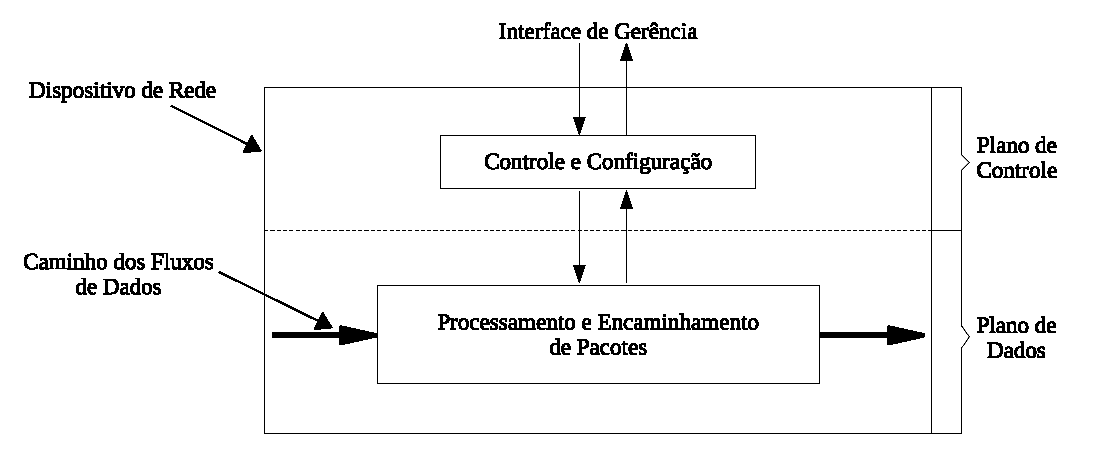
\includegraphics[width=.9\textwidth]{images/planos-introducao.eps}
  \fonte{Comer, 2013. \nocite{Comer:2013}}
  \label{fig:planos-introducao}
  
\end{figure}
\FloatBarrier

Para tentar contornar esse problema, a comunidade de pesquisa em redes de computadores tem investido em iniciativas que levem a implantação de redes com maiores recursos de programação, de forma que novas tecnologias possam ser inseridas na rede de forma gradual. Exemplos de iniciativas desse tipo são as propostas de redes ativas (\textit{active networks}) \cite{Tennenhouse:1997}, de \textit{testbeds} como o PlanetLab \cite{Chun:2003}, GENI \cite{Turner:2006} e, mais recentemente o FIBRE \cite{Salmito:2014}. Redes ativas, tiveram pouca aceitação pela necessidade de alteração dos elementos de rede para permitir que se tornassem programáveis. Iniciativas mais recentes como PlanetLab, GENI e FIBRE, apostam na adoção de recursos de virtualização para facilitar a transição para novas tecnologias. Apesar de serem consideradas de grande potencial a longo prazo, tais iniciativas ainda enfrentam desafios como garantir o desempenho exigido pelas aplicações utilizadas hoje utilizando-se tais elementos virtualizados \cite{Guedes:2006}.

Uma outra forma de abordar esse problema, consiste em estender o \textit{hardware} de encaminhamento de pacotes de forma mais restrita. Considerando-se que a operação que necessita de alto desempenho nos elementos de comutação é o encaminhamento de pacotes (plano de dados), algumas iniciativas propõem manter essa operação pouco alterada, para manter a viabilidade de desenvolvimento de hardware de alto desempenho, mas com uma possibilidade de maior controle por parte do administrador da rede. 

\gls{sdn} introduz uma perspectiva flexível para programar e manter a operacionalidade da rede  buscando desacoplar os planos de dados e de controle, desta forma, tira-se a autonomia dos equipamentos de rede que se tornam apenas encaminhadores de pacotes. Já a lógica de controle é movida para uma entidade externa, centralizada, implementada em \textit{software}. Esta, chamada de controlador, tem por funcionalidade prover a lógica de funcionamento da rede o que torna o desenvolvimento de serviços mais facilmente implementáveis, já que não há a necessidade de implementação em cada dispositivo. 

No plano de dados, o encaminhamento de pacotes, que antes era baseado em destino, passa a ser por fluxo que é definido pela combinação de campos das camadas de enlace, de rede ou de transporte, segundo o modelo TCP/IP. Dessa forma mantém-se o alto desempenho no encaminhamento de pacotes em \textit{hardware}, aliado à flexibilidade de se implementar aplicações em \textit{software}, utilizando protocolo aberto para programação da lógica do equipamento que é abstraída dos dispositivos de encaminhamento \cite{Kim:2013, Tootoonchian:2010, Rothenberg:2010}.

Pensando nisso, nasceu o OpenFlow \cite{McKeown:2008}, que por sua vez, deu origem ao conceito de \textit{Software Defined Networking}, ou redes definidas por software. A Figura \ref{fig:arch-old-sdn} apresenta um comparativo entre o modelo tradicional de rede, onde ambos os planos, de controle e de dados, são localizados em um mesmo dispositivo e o modelo \gls{sdn} que possui controle centralizado e apenas o plano de dados no dispositivo comutador.

\begin{figure}[H]
  \centering
  \caption{Modelos de rede tradicional e SDN}
  \includegraphics[width=.80\textwidth]{images/arch-old-sdn.eps}
  \fonte{Rothenberg \textit{et al.}, 2010. \nocite{Rothenberg:2010}}
  \label{fig:arch-old-sdn}
\end{figure}
\FloatBarrier

O protocolo OpenFlow é implementado em ambos os planos e dispõe de um protocolo de comunicação entre o controlador e \textit{switches}. Para garantir a confiabilidade dessa comunicação é recomendada a utilização do protocolo \gls{ssl} \cite{RFC6101} porém algumas alternativas incluem \gls{tcp}, utilizadas especialmente em redes virtuais devido à sua simplicidade, pois não necessitam de chaves criptográficas \cite{Rothenberg:2010}.

OpenFlow explora a existência de tabelas de fluxo (\textit{flow tables}) em dispositivos \textit{Ethernet} modernos. Essas tabelas são alimentadas em tempo de execução e utilizadas para implementar \textit{firewalls} \cite{Oppliger:1997}, \gls{nat} \cite{RFC3022}, \gls{qos} \cite{Aurrecoechea:1998} e coleta de estatísticas. Normalmente são proprietárias mas há um conjunto de funções que são comuns na maioria dos dispositivos. Com isso, uma forma padrão de manipulação das tabelas de fluxo pode ser implementada, independente de fornecedor. Desta maneira, OpenFlow fornece um padrão para manipulação das tabelas de fluxo, permitindo assim a partição do tráfego, o agrupamento ou isolamento da rede e o processamento ou controle do fluxo de dados, da forma desejada com base no fluxo \cite{Kontesidou:2009}.

Os principais componentes de uma arquitetura \gls{sdn} são:
\begin{itemize}
    \item Comutadores (\textit{switches}) \textit{OpenFlow};
    \item Controlador; e
    \item Protocolo de comunicação.
\end{itemize}
Estes componentes podem fazer uso do protocolo OpenFlow e/ou de outros protocolos. Por ser o primeiro e também o mais utilizado, o protocolo OpenFlow é utilizado neste trabalho como padrão de comunicação entre os dispositivos.

%=====================================================================

\subsection{Comutadores}
\label{subsec:comutador}

É o elemento responsável pelo encaminhamento dos pacotes pela rede. Pode ser específico para OpenFlow, ou ter suporte ao mesmo. No comutador (\textit{switch}) OpenFlow é mantida uma tabela de fluxo (\textit{flow table}) que armazena informações sobre como os pacotes serão processados, estatísticas, prioridades e tempo limite para novos fluxos. Além disso, cada regra é composta por um conjunto de campos do cabeçalho do pacote que podem ser visualizadas na Figura \ref{fig:flow-table}, assim como as informações de ações e estatísticas.

\begin{figure}[H]
  \centering
  \caption{Tabela de fluxo}
  \includegraphics[width=.65\textwidth]{images/flow-table.eps}
  \label{fig:flow-table}
  \fonte{Adaptado de Costa, 2014 \nocite{Costa:2004}}
\end{figure}
\FloatBarrier
%Copiado e artigo 6, reescrever
Quando um pacote chega a um equipamento com OpenFlow habilitado, os cabeçalhos do pacote são comparados (\textit{match}) às regras das entradas das tabelas de fluxos, os contadores são atualizados e as ações correspondentes são realizadas. Se não houver correspondência  (\textit{table miss}) entre o pacote e alguma entrada da tabela de fluxos, o pacote é encaminhado, por completo, ao controlador. Alternativamente, apenas o cabeçalho é encaminhado ao controlador mantendo o pacote armazenado no \textit{buffer} do \textit{hardware}. A Figura \ref{fig:fluxo-tmp} ilustra, através de um diagrama simplificado, o tratamento recebido por pacotes em um \textit{switch} OpenFlow.

Os pacotes que chegam ao controlador normalmente correspondem ao primeiro pacote de um novo fluxo ou, em função do tipo de pacote e da aplicação, o controlador pode decidir por instalar uma regra no \textit{switch} para que todos os pacotes de determinado fluxo sejam enviados para o controlador para serem tratados individualmente. Esse último caso corresponde, em geral, a pacotes de controle  (\gls{icmp} \cite{RFC0792}, \gls{dns} \cite{RFC7719}, \gls{dhcp} \cite{RFC2131}) ou de protocolos de roteamento  (\gls{ospf} \cite{RFC2328}, \gls{bgp} \cite{RFC4271}).
Todos os pacotes de uma mesma faixa de endereços \gls{ip}, ou uma conexão \gls{tcp} em determinada porta são considerados fluxos.

\begin{figure}[H]
  \centering
  \caption{Diagrama simplificado do tratamento de um pacote no \textit{switch} OpenFlow}
  \includegraphics[width=.80\textwidth]{images/flow.eps}
  \label{fig:fluxo-tmp}
  \fonte{Elaborado pelo autor a partir da especificação OpenFlow\\\cite{OpenFlowSpec:2014}}
\end{figure}
\FloatBarrier

A cada pacote recebido, é realizada a atualização dos contadores na tabela de fluxo.
Esses contadores são usados para geração de estatísticas, de maneira a monitorar o número de pacotes e bytes de cada fluxo, além do tempo de duração desde o seu início. O Quadro \ref{tab:contadores} apresenta alguns dos contadores disponíveis na tabela de fluxo. Com o auxílio deste podem ser implementados recursos de monitoramento e segurança do tráfego na rede.

\begin{table}[H]
  \centering
  %\captionof{figure}[tab:contadores]{Contadores da tabela de fluxo}
  \caption{Contadores da tabela de encaminhamento}
  \begin{tabular}{|l|c|} \hline
	\textbf{Contator} & \textbf{Tamanho em bits} \\ \hline
	\multicolumn{2}{|c|}{Por Tabela} \\ \hline
	Número de entradas Ativas & 32 \\ \hline
	Número de pacotes pesquisados & 64 \\ \hline
	Número de pacotes encontrados na tabela & 64 \\ \hline
	\multicolumn{2}{|c|}{Por fluxo} \\ \hline
	Número de pacotes recebidos & 64 \\ \hline
	Número de bytes recebidos & 64 \\ \hline
	Duração (segundos) & 32 \\ \hline
	Duração (nano segundos) & 32 \\ \hline
	\multicolumn{2}{|c|}{Por porta} \\ \hline
	Número de pacotes recebidos & 64 \\ \hline
	Número de pacotes transmitidos & 64 \\ \hline
	Número de bytes recebidos & 64 \\ \hline
	Número de bytes transmitidos & 64 \\ \hline
	Número de pacotes perdidos no recebimento & 64 \\ \hline
	Número de pacotes perdidos na transmissão & 64 \\ \hline
	Número de erros recebidos & 64 \\ \hline
  \end{tabular}
  \label{tab:contadores}
  \fonte{Elaborado pelo autor a partir da especificação OpenFlow\\  \cite{OpenFlowSpec:2014}}
\end{table}

Neste projeto o comutador a ser utilizado é o Open vSwitch \cite{website:ovs}, um \textit{switch} virtual com suporte a OpenFlow. Este comutador é projetado para permitir a automatização de grandes redes através da extensão programática, suportando ainda interfaces e protocolos de gerenciamento como, por exemplo, NetFlow \cite{rfc3954}, sFlow \cite{rfc3176} e IPFIX \cite{rfc5153}. Além disso, pode suportar a distribuição através de múltiplos servidores físicos \cite{website:ovs}.
%=====================================================================

\subsection{Controlador}
\label{subsec:controlador}

O controlador, como já citado, é o \textit{software} responsável por tomar decisões e adicionar e remover as entradas na tabela de encaminhamento, de acordo com o objetivo desejado. Exerce a função de uma camada de abstração da infraestrutura física, facilitando a criação de aplicações e serviços que gerenciem as entradas de fluxos na rede. Esse modelo assemelha-se a outros sistemas de \textit{software} que proveem abstração do \textit{hardware} e funcionalidade reutilizável. Dessa forma, o controlador atua como um \gls{so} para gerenciamento e controle das redes, e oferece uma plataforma com base na reutilização de componentes e na definição de níveis de abstração. Contudo, novas aplicações de rede podem ser desenvolvidas rapidamente \cite{Gude:2008}.

O controlador fornece uma interface para criar, modificar e controlar o fluxo de tabelas do comutador. É executado normalmente em um servidor conectado à rede e pode ser um para todos os comutadores da rede, um para cada comutador ou um para um conjunto de comutadores.  Portanto, a funcionalidade da rede de controle pode ser completamente ou localmente centralizada dependendo de como o gerenciamento dos comutadores é realizada. A exigência, no entanto, é que, se houver mais do que um controlador de processos, eles devem ter a mesma visão da topologia da rede, em qualquer momento dado. A visão de rede inclui a topologia a nível de \textit{switch}, as localizações dos usuários, \textit{hosts}, \textit{middleboxes} e outros elementos de rede e serviços. Além disso inclui todas as ligações entre os nomes e endereços.

O controlador é parte integrante de uma arquitetura de rede \gls{sdn} e para que sua comunicação com \textit{switches} OpenFlow ocorra, o controlador deve ter suporte ao mesmo. Atualmente, existem várias implementações controlador disponíveis que implementam o protocolo OpenFlow, entre os principais não comerciais estão \cite{Kreutz:2013,Xia:2015}:

\begin{itemize}
    \item \textbf{NOX} - Desenvolvido em C++, foi o primeiro controlador OpenFlow \cite{Gude:2008}. Porém não foi fortemente utilizado por causa de deficiências na sua implementação e na documentação.
    \item \textbf{POX} - Sucessor do NOX, foi desenvolvido como uma alternativa mais amigável e tem sido implementado por um grande número de engenheiros e programadores \gls{sdn}. Comparando com NOX, POX tem um ambiente de desenvolvimento mais fácil de trabalhar com uma API razoavelmente bem escrita e documentada. Também fornece uma interface Web e é escrito em Python \cite{website:pox}.
    \item \textbf{Beacon} - É um controlador SDN bem escrito e organizado. Escrito em Java, Beacon foi o primeiro controlador com o qual iniciantes pudessem trabalhar e criar um ambiente \gls{sdn}, no entanto, era limitado à topologias de rede estrela \cite{Erickson:2013}.
    \item \textbf{Floodlight} - Uma ramificação do Beacon. Enquanto que seu início tenha sido baseado no Beacon este foi desenvolvido utilizando Apache Ant, uma ferramenta popular para compilação e construção de \textit{software}, o que tornou o desenvolvimento do Floodlight mais fácil e flexível. Floodlight possui uma comunidade ativa e um grande número de recursos que podem ser adicionados ao sistema. Possui interface baseada em java e baseada em Web, além de possuir uma Interface de Programação de Aplicações (\gls{api}) \gls{rest} ou, em português, Transferência de Estado Representacional \cite{website:floodlight}.
    \item \textbf{OpenDayLight} - É um projeto colaborativo da Linux Fundation e tem sido altamente suportado por empresas como Cisco e Big Switch. Desenvolvido em Java, também inclui \gls{api} \gls{rest} e interface web. Possui suporte à \gls{sdn}, \gls{nv} , ou Virtualização de redes \cite{Chowdhury:2009} e \gls{nfv}, ou Virtualização da Funções da Rede \cite{Hawilo:2014}. Além disso, possui um grande número de módulos que podem ser utilizados para atender aos requisitos de uma organização \cite{website:odl}.
    \item \textbf{Ryu NOS} - É um \textit{framework} de \gls{sdn} baseado em componentes. O Ryu fornece componentes de software com \glspl{api} bem definidas que tornam mais fácil para os desenvolvedores criar novas aplicações de gerenciamento e controle de rede. O Ryu suporta vários protocolos para gerenciar dispositivos de rede, como OpenFlow, Netconf, OF-config, etc. Sobre o OpenFlow, o Ryu suporta totalmente as extensões 1.0, 1.2, 1.3, 1.4, 1.5 e Nicira. Todo o código está disponível gratuitamente sob a licença Apache 2.0 \cite{website:ryu}.
\end{itemize}

%=====================================================================

\subsection{Protocolo OpenFlow}
\label{subsec:protocolo-comunicacao}

O protocolo de comunicação entre os dois planos é realizado por três tipos de mensagens: controlador para o \textit{switch}, assíncrona e simétricas. 

Mensagens do tipo controlador para \textit{switch} são mensagens que o controlador envia para obter informações sobre o estado do \textit{switch}, como por exemplo verificar estatísticas de um determinado fluxo \cite{OpenFlowSpec:2014}. Essas mensagens podem ser:
%Rescrever
\begin{itemize}
    \item \textit{\textbf{Features}}: ao estabelecer uma conexão, o controlador envia esta mensagem requisitando que o \textit{switch} informe suas capacidades.
    \item \textit{\textbf{Configuration}}: o controlador envia parâmetros de configuração para os \textit{switches}. 
    \item \textit{\textbf{Modify-State}}: utilizado pelo controlador para gerenciar o estado dos \textit{switches}, deletar ou modificar regras na tabela de fluxos.
    \item \textit{\textbf{Read-State}}: utilizado pelo controlador para coletar estatísticas das tabelas de fluxos do \textit{switch}.
    \item \textit{\textbf{Packet-Out}}: utilizada pelo controlador para enviar pacotes por uma porta específica.
    \item \textit{\textbf{Barrier}}: utilizada para verificar se as dependências das mensagens foram alcançadas ou receber notificação sobre tarefas concluídas.
     \item \textit{\textbf{Role Request}}: mensagens usadas pelo controlador para configurar seu canal OpenFlow.
\end{itemize}

Mensagens assíncronas são enviadas pelo \textit{switch} sem a solicitação do controlador. \textit{Switches} enviam mensagens assíncronas para os controladores para denotar uma chegada de pacotes ou mudança de estado \cite{OpenFlowSpec:2014}. Os principais tipos de mensagens assíncronas são descritas abaixo.
\begin{itemize}
    \item \textit{\textbf{Packet-In}}: enviado pelo \textit{switch} quando há uma ação explícita na tabela de fluxos para que seja enviado para o controlador ou quando não há um \textit{match} para o pacote.
    \item \textit{\textbf{Flow-Removed}}: informa o controlador sobre a remoção de regras no \textit{switch}.
    \item \textit{\textbf{Port Status}}: informa o controlador sobre uma mudança em alguma porta.
    \item \textit{\textbf{Role Status}}: \textit{switch} informa o controlador sobre a alterações em suas regras.
    \item \textit{\textbf{Controller Status}}: \textit{switch} informa o controlador sobre a mudança em um canal OpenFlow.
    \item \textit{\textbf{Flow-monitor}}: informa o controlador sobre uma mudança na tabela de fluxo.
\end{itemize}

Finalmente, mensagens simétricas são iniciadas tanto pelo controlador como pelo \textit{switch} sem nenhuma solicitação, por exemplo o início de conexão entre controlador e \textit{switch} \cite{OpenFlowSpec:2014}. Essas mensagens são:
\begin{itemize}
    \item \textit{\textbf{Hello}}: esta mensagem é utilizada no início da conexão entre \textit{switch} e controlador.
    \item \textit{\textbf{Echo}}: utilizado para obter informações sobre a conexão entre \textit{switch} e controlador como:
latência, largura de banda e conectividade.
    \item \textit{\textbf{Error}}:  o \textit{switch} pode enviar mensagens para notificar problemas ao controlador por mensagens de erro.
    \item \textit{\textbf{Experimenter}}: na versão 1.5.0 do protocolo OpenFlow, esta mensagem é utilizada para adicionar funcionalidades experimentais.
\end{itemize}

Cada mensagem é enviada encapsulada em um pacote definido pelo protocolo OpenFlow e que é representado na Figura \ref{fig:openflow-message}.

\begin{figure}[H]
  \centering
  \caption{Formato da mensagem OpenFlow}
  \includegraphics[width=.80\textwidth]{images/openflow-message.eps}
  \label{fig:openflow-message}
  \fonte{\centering
  Elaborado pelo autor a partir de informações da especificação OpenFlow.}
\end{figure}
\FloatBarrier

O campo \textit{version} indica a versão do protocolo que está sendo utilizada. Já o  \textit{type}, indica o tipo de mensagem que está sendo enviada. O campo \textit{length} informa o tamanho da mensagem enquanto que \textit{xid} representa o ID de transação associado à mensagem. Por último, o campo \textit{payload} representa o corpo da mensagem, é neste campo onde são adicionados os diferentes tipos de mensagens apresentados anteriormente.
\section{Virtualização}
\label{sec:virtualizacao}
%Rescrever

O conceito de virtualização de redes define uma infraestrutura de redes de computadores virtuais. São definidos por \textit{software}, executando sobre máquinas físicas, de forma que toda infraestrutura virtual seja isolada da infraestrutura física, não interferindo na mesma. 

Um dos \textit{softwares} mais usados na criação de redes virtuais em nível de \textit{software} é o Xen \cite{Fernandes:2011}. Esse programa é usado na criação de máquinas virtuais em computadores pessoais e servidores, e oferece a opção de criar roteadores virtuais que podem ser utilizados na interligação de máquinas virtuais para a formação de uma rede. Em \gls{sdn} a construção de redes virtuais acontece em nível de \textit{hardware}, através da separação do tráfego da rede física em \textit{slices}, porções de fluxo do tráfego total. O FlowVisor \cite{Sherwood:2009} possibilita virtualização em \gls{sdn}.

O uso de virtualização de redes possibilita execução de experimentos distintos, sobre a mesma infraestrutura, em paralelo, sem interferência entre experimentos. Virtualização de redes também pode ser usada para isolamento de serviços. Assim, uma organização pode oferecer diversos serviços, com cada serviços executando em uma rede virtual diferente \cite{wu:2010, Mattos:2012}.

\section{Emulador Mininet}
\label{sec:mininet}

Mininet \cite{Handigol:2012} é um emulador de rede para prototipação em \gls{sdn}. A razão pela sua utilização deve-se ao fato de apenas alguns dispositivos de rede estarem disponíveis para \gls{sdn}, uma vez que ainda não é uma tecnologia difundida a nível industrial.  Além disso, a implementação de rede com elevado número de dispositivos de rede é muito difícil e dispendioso. Por isso, para contornar estes problemas, a virtualização foi realizada com a finalidade de prototipar e emular este tipo de tecnologia de rede e um dos mais importantes é o Mininet \cite{Wendong:2012}.  Mininet tem a capacidade de emular diferentes tipos de elementos de rede, tais como: \textit{host}, \textit{switches} (camada de enlace), roteadores (camada de rede) e conexões. Ele funciona em um único núcleo de Linux\cite{Negus:2015} e utiliza virtualização com a finalidade de emular uma rede completa que utiliza apenas um único sistema. No entanto, o \textit{host}, roteadores e links criados são elementos do mundo real, embora eles sejam criados por meio de software \cite{website:mininet}.

Criar uma rede no Mininet é relativamente simples. Pode-se usar linha de comando ou um componente chamado \textit{miniedit.py}, que implementa uma interface gráfica para o Mininet, este porém, possui algumas limitações em relação à linha de comando. Pela linha de comando, ao chamar o Mininet são passados os parâmetros sobre as características da rede como: topologia, número de \textit{hosts}, \textit{switches}, taxa de perda de pacotes, largura de banda, tipo de controlador, entre outros. O \textit{switch} padrão é o OpenSwitch \cite{Pettit:2010}, um \textit{switch} virtual desenvolvido especialmente para trabalhar com o protocolo Openflow. Para estudo mais aprofundado, recomenda-se a leitura da sua documentação em \cite{website:mininet}.
\section{Segurança em redes}
\label{sec:seguranca}

A segurança no nível de rede indica uma área de pesquisa muito importante, já que os usuários estão continuamente colocando seus dados em ambientes em nuvem e mais dados são transferidos através de grandes distâncias. A razão para esta evolução é a crescente popularidade dos serviços em nuvem, bem como a simplicidade e rápida capacidade dos recursos sob demanda. Os impactos variam de acordo com os tipos de ameaças, e como defesa são criados diversos sistemas de segurança que agem como barreira de proteção, como por exemplo, \textit{firewalls}. Os principais tipos de ameaças serão estudadas a seguir. Também é apresentado um estudo mais detalhado do ataque do tipo varredura, foco deste trabalho.

\subsection{Tipos de ameaças}
Dos diversos tipos de ameaças que podem ocorrer nas redes de computadores, destacam-se algumas que são notórias por causar frequentes transtornos aos usuário, tais como:

\textbf{Fraude}:
Segundo Houaiss, Villar e Francisco (2001)\nocite{Houaiss:2001}, é "qualquer ato ardiloso, enganoso, de má-fé, com intuito de lesar ou ludibriar outrem, ou de não cumprir determinado dever; logro". Esta categoria engloba as notificações de tentativas de fraudes, ou seja, de incidentes em que ocorre uma tentativa de obter vantagem, sejam por meios como correios eletrônicos não solicitados em massa (\textit{spam}) e páginas falsas.
    
\textbf{Ataque de negação de serviço (\textit{\gls{dos}}}:
Um ataque de negação de serviço busca sobrecarregar serviços na rede dificultando o seu uso por usuários legítimos. Esse tipo de ataque, por sua natureza, pode produzir variações no volume de tráfego que normalmente são visíveis no gráfico de fluxo. Segundo Sperotto \textit{et al.} (2010)\nocite{Sperotto:2010} no entanto, na detecção de intrusão por fluxo, é abordado implicitamente o problema de ataques \gls{dos} por força bruta, ou seja, um tipo de \gls{dos} que depende de esgotamento de recursos ou sobrecarga da rede. Infelizmente, é quase impossível de detectar diretamente ataques \gls{dos} semânticas.
    
\textbf{Infestações viróticas automatizadas (\textit{Worms})}:
São pequenos programas de computador criados para causar danos na máquina infectada e se auto replica pela rede, tirando cópias de si em cada computador \cite{Sperotto:2010}.
    
\textbf{Exército de máquinas controladas sem autorização (\textit{Botnets})}:
Grupo de computadores comprometidos, chamados de computadores zumbis que são controlados remotamente por um centro de controle. \textit{Botnets} são muito utilizados para lançamento de ataques  como \textit{spams}, DoS e \textit{worms} \cite{Sperotto:2010}.
    
\textbf{Varredura de portas maliciosa (\textit{port scans})}:
Técnica utilizada para encontrar fraquezas de um computador ou de uma rede. Enquanto esta técnica não é um ataque real, os hackers a usam para detectar quais portas estão abertas em um computador. Baseado nas informações sobre portas abertas, o acesso não autorizado pode ser obtido.

Os métodos citados também podem também ser utilizados em conjunto, como por exemplo a utilização de \textit{botnets} que, controlados remotamente, podem efetuar ataques DoS a um mesmo servidor e ao mesmo tempo. A esse tipo de ataque é dado o nome de Negação de Serviço Distribuída (\gls{ddos})

Do ponto de vista de segurança, existe uma quantidade crescente de incidência de ataques de negação de serviço, \gls{dos}, durante os últimos anos \cite{Seeber:2015}. Além disso, segundo a \gls{cert.br}, responsável por tratar incidentes de segurança e computadores que envolvam redes conectadas à Internet brasileira, foram reportados 722.205 incidências de segurança somente no ano de 2015, sendo mais da metade (53\%), ataques do tipo \textit{port scan}.

\subsection{Técnicas de varredura}
\label{sec:varredura}

Um dos tipos mais comuns de ataques, a varredura consiste no envio de diversos tipos de pacotes com o intuito de se conhecer mais sobre o nó alvo ou a rede em questão. Através das respostas obtidas para esses pacotes, o atacante é capaz de chegar a diversas informações que possam ajudar em futuros ataques de diversos tipos. Alguns tipos de informações que podem ser descobertas incluem (não somente): A atividade dos servidores, informações relativas a softwares utilizados no sistema, informações sobre o \textit{firewall} e topologia da rede.

Uma das principais dificuldades nas soluções desse tipo de ataque é que as varreduras são consideradas atividades legais, e ocorrem na Internet de forma rotineira, inclusive com fins não maliciosos.

Antes de explorar as técnicas de varredura, faz-se necessário o entendimento de alguns conceitos de comunicação \gls{tcp}. Para obter um serviço \gls{tcp}, uma conexão necessita ser efetivada entre os computadores origem e destino. Esta conexão é realizada através dos chamados \textit{sockets}, formados pelo par endereço \gls{ip} e número de porta, de ambos, computador de origem e computador de destino. Entre estes dois \textit{sockets} ocorre a transferência de segmentos.

Um segmento consiste em um cabeçalho \gls{tcp} seguido, opcionalmente, por informação. Um cabeçalho \gls{tcp} pode possuir seis \textit{flags} que podem ser ativadas ou desativadas ao mesmo tempo \cite{Comer:2013}, são elas:

\begin{itemize}
    \item \textbf{SYN} - \textit{bit} de sincronismo, é o \textit{bit} que informa que este é um dos dois primeiros segmentos de estabelecimento da conexão.
    \item \textbf{ACK} - \textit{bit} de reconhecimento, indica que o valor do campo de reconhecimento está carregando um reconhecimento válido.
    \item \textbf{PSH} - \textit{bit} de \textit{push}, este mecanismo, que pode ser acionado pela aplicação, informa ao \gls{tcp} origem e destino que a aplicação solicita a transmissão rápida dos dados enviados, mesmo que ela contenha um número baixo de \textit{bytes}, não preenchendo o tamanho mínimo do \textit{buffer} de transmissão.
    \item \textbf{RST} - \textit{bit} de \textit{reset}, informa o destino que a conexão foi abortada neste sentido pela origem
    \item \textbf{FIN} - \textit{bit} de terminação, indica que este pacote é um dos pacotes de finalização da conexão.
\end{itemize}

Em uma comunicação \gls{tcp}, uma conexão deve ser estabelecida entre os dois pontos (\textit{sockets}) para que a transferência de dados ocorra.
Inicialmente a máquina emissora, também chamada de cliente, transmite um segmento cuja \textit{flag} SYN é de 1 (para assinalar que se trata de um segmento de sincronização), com um número de ordem X, que se chama número de ordem inicial do cliente.

A seguir, a máquina receptora, chamada de servidor, recebe o segmento inicial que provém do cliente e envia-lhe um aviso de recepção, isto é, um segmento cuja \textit{flag} ACK é de 1 e a \textit{flag} SYN é de 1 (porque ainda se trata de uma sincronização). Este segmento contém o número de ordem do servidor, que é o número de ordem inicial do cliente. O campo mais importante deste segmento é o campo de aviso de recepção, que contém o número de ordem inicial do cliente, incrementado de 1.

Por último, o cliente transmite ao servidor um aviso de recepção, ou seja, um segmento cuja \textit{flag} ACK é de 1, cuja \textit{flag} SYN é de zero (não se trata mais de um segmento de sincronização). O seu número de ordem é incrementado e o número de aviso de recepção representa o número de ordem inicial do servidor, incrementado de 1.

Depois dessa sequência de trocas (Figura \ref{fig:troca-tcp}), também chamada de \textit{handshake}, ou, aperto de mãos em português, as duas máquinas estão conectadas e a comunicação pode ser efetivada.

\begin{figure}[H]
  \centering
  \caption{Estabelecimento de conexão TCP}
  \includegraphics[width=0.5\textwidth]{images/conexao-tcp.eps}
  \label{fig:troca-tcp}
   \fonte{Elaborado pelo autor.}
\end{figure}
\FloatBarrier

Os passos a seguir são definidos pela RFC 793 \cite{rfc793}, utilizada pela grande maioria das implementações \gls{tcp} e exploradas em técnicas de varredura.

\begin{itemize}
    \item Quando um segmento SYN chega em um aporta aberta, é continuado o procedimento de \textit{handshake} como discutido anteriormente; 
    \item Quando um segmento SYN (ou FIN) chega em uma porta fechada, o segmento é descartado e um segmento RST é retornado para o cliente;
    \item Quanto um segmento FIN chega em uma porta que esteja aberta, o segmento é descartado.
    \item Quando um segmento RST chega em uma porta que esteja ouvindo (aberta), o segmento é descartado;
    \item Quando um segmento RST chega em uma porta que não esteja ouvindo (fechada), o segmento é descartado;
    \item Quando um segmento ACK chega à uma porta aberta, o mesmo é descartado e retornado um segmento RST.
\end{itemize}


Devido à sua natureza, \textit{scans} podem facilmente criar um vasto número diferente de fluxos. Segundo Speroto \textit{et al.} (2010)\nocite{Sperotto:2010}, há três categorias de varredura, são elas:
\begin{itemize}
    \item \textbf{\textit{scan} horizontal} - quando um \textit{host} de origem varre uma porta especifica em diferentes \textit{hosts} alvo;
    \item \textbf{\textit{scan} vertical} - quando um \textit{host} de origem verifica várias portas distintas de um mesmo \textit{host} alvo; e
    \item \textbf{\textit{scan} misto} - quando há a combinação das varreduras vertical e horizontal.
\end{itemize}

Existem várias técnicas de varredura de porta disponíveis e podem facilmente ser automatizadas por ferramentas como Nmap \cite{Lyon:2009}. Alguns métodos utilizados para varredura são estudados a seguir \cite{deVivo:1999, Christopher:2001}.
\begin{itemize}
\item \textbf{\textit{TCP Connect}} - É a forma mais comum de \textit{scanning}. Basicamente uma conexão TCP regular (\textit{handshake} completo) para cada porta definida na varredura. Para cada porta, a conexão pode resultar em sucesso, indicando uma porta aberta ou em falha caso contrário. Essa técnica é facilmente implementada pois não necessita de privilégios especiais e, do mesmo modo, é facilmente detectável. Através de \textit{logs} do sistema alvo é possível verificar mensagens de requisição de conexão e de erro para as conexões negadas. Neste método, o \textit{scanner} envia uma mensagem SYN para o sistema alvo. Se uma porta estiver (aberta) ouvindo com um serviço, a conexão se sucederá. Um SYN é retornado estabelecendo o número de sequência inicial. Um ACK considera o campo numérico de confirmação válido. Se a porta estiver (fechada) sem serviço ouvindo, uma mensagem RST é retornada, para reiniciar o pedido de conexão. Alguns exemplos de \textit{scanners} podem ser Nmap, Amap e Blaster. %Exemplo de \textit{scanner}: nmap.

\item \textbf{TCP SYN} - Também conhecida por \textit{Half Open} por não explorar um \textit{handshake} completo. Nesta técnica o \textit{scanner} envia uma mensagem SYN, como se estivesse pedindo uma conexão. Se responder como um RST, indica que a porta está fechada, e uma nova porta é testada. Se a resposta da máquina alvo for um SYN/ACK, indica que a porta se encontra ouvindo. O \textit{scanner} envia então um RST cancelando o \textit{handshake}. A vantagem desse tipo de \textit{scanning} é o fato de, mesmo ainda podendo ser detectado, tentativas de conexões SYN são menos frequentemente registradas se comparadas com conexões \gls{tcp} completas. %Exemplos de \textit{scanners}: amap, hping2, netstat, nmap.

\item \textbf{Exploração FIN} - Neste método, quando um segmento FIN é enviado para uma porta fechada, o computador alvo responde com um TCP RST. Quando a porta estiver aberta, o segmento é ignorado e o computador alvo não responde. O \textit{scanner} não recebe nunhuma resposta, pois não podem pertencer a uma conexão estabelecida. %Exemplos de \textit{scanners}: hping2, nmap.

\item \textbf{Xmas Tree} - é uma variação do método TCP FIN, neste, são utilizadas mensagens com prioridade TCP FIN/URG/PSH. Quando estiver ouvindo, o \textit{host} alvo não responde, caso contrário, responde com um TCP RST. %Exemplos de \textit{scanners}: hping2, netstat, nmap.

\item \textbf{TCP Null (sem flags ativos)} - também é uma variação do método TCP FIN, neste, tem-se resposta para portas fechadas, mas não para portas abertas.% Exemplos de \textit{scanners}: hping2, netstat, nmap.

\item \textbf{Varredura ACK} - Técnica utilizada para identificar \textit{firewalls}. Um segmento ACK que não pertença a nenhum conexão é gerado pelo \textit{scanner}. Se um RST é devolvido pela máquina alvo, tanto em uma porta aberta como em uma fechada, as portas são classificadas como não tendo \textit{firewall}.

\item \textbf{Varredura ARP} - Não se trata exatamente de varredura de portas mas essa técnica é utilizada para descobrir dispositivos ativos na rede local, para depois realizar a varredura de portas somente nos computadores ativos. O \textit{scanner} envia uma série de pacotes de protocolo \gls{arp} \cite{RFC0826} e incrementa o valor do \gls{ip} alvo a cada \textit{broadcast}.
\end{itemize}


\subsection{Ferramentas de Varredura}

Para que as varreduras sejam efetuadas, tem-se a possibilidade de utilizar ferramentas que possibilite a varredura utilizando as diferentes formas citadas na seção anterior. Uma das ferramentas mais utilizadas, e que foi utilizada neste trabalho é o Nmap \cite{Lyon:2009}.

O Nmap é um \textit{software} que oferece uma gama muito grande de recursos e funcionalidades, como detecção do Sistema Operacional remoto, o serviço e a versão que está em uso no host, o exame de ociosidade por identificação (ID) de Internet Protocol (IP), o rápido exame de multiportas por ping entre tantas outras. Possui versões para plataformas Unix, Windows, e MacOS sendo utilizado tanto por interface console como também em interface gráfica, o software Nmap é um utilitário livre e de código aberto, usado para exploração de redes, segurança e auditoria, capaz de examinar grandes redes ou simplesmente um único host.
A função principal do Nmap é realizar uma varredura em portas \gls{tcp} e o retorno dessa varredura é classificado em um dos seguintes estados: aberta, fechada, filtrada, nao filtrada e a combinação de aberta/filtrada ou fechada/filtrada \cite{Lyon:2009}. Vários outros softwares que são utilizados para gerencia e controle de redes de computadores fazem uso do Nmap pois pode ser usado diretamente, sempre que se desejar uma verificação de portas em um \textit{host} que esteja em uma rede local ou na Internet.
O uso mais simples do Nmap é escanear diretamente uma máquina da rede, onde uma quantidade enorme de portas \gls{tcp} será examinada na máquina alvo, e cada porta será classificada de acordo com seu estado.
Na linha de comando do Nmap, tudo que não for uma opção ou argumento de opção será tratado como uma especificação de hospedeiro alvo. O caso mais simples é a especificação de um endereço IP ou nome de hospedeiro alvo para exame \cite{Lyon:2009}.


\subsection{Sistemas de detecção e prevenção de intrusão}

O isolamento da rede em redes virtuais permite uma maior segurança devido ao seu isolamento, porém problemas tradicionais relacionados à segurança continuam existindo em ambientes virtualizados pois 60\% a 70\% dos ataques à segurança da rede são de origem interna segundo Lynch (2006)\nocite{Lynch:2006}. Uma das formas de se proteger desses ataques é monitorar o tráfego em busca de atividades maliciosas ou violação de políticas. Para realizar o monitoramento de pacotes na rede, a solução mais apropriada é o sistema de detecção de intrusão, que realiza o monitoramento passivo dos pacotes na rede. Porém, esse tipo de análise não permite que sejam tomadas ações para prevenir tais ataques, e então faz se necessário um sistema de prevenção de intrusão para bloquear esses pacotes.

Segundo Kruegel (2004)\nocite{Kruegel:2004}, "Detecção de intrusão é o processo de identificar e responder à atividades maliciosas na computação e redes de dados". Uma tentativa de intrusão, também chamada de ataque, refere-se a uma série de ações em que um intruso tenta obter o ganho do sistema e o objetivo de um \gls{ids} é discriminar tentativas de intrusão e preparação de intrusão do uso normal do sistema.

Em redes tradicionais, para detectar e prevenir intrusos maliciosos na rede de dados, administradores normalmente necessitam implantar diversos detectores de intrusão em diferentes locais da rede, e então analisar dados do tráfego coletados localmente ou em um nodo centralizado. Infelizmente, arquiteturas \gls{ids}/\gls{ips} utilizadas atualmente possuem muitas barreiras para gerir nós distribuídos. Em primeiro lugar, os nós de detecção de intrusão devem suportar diferentes configurações. Como as configurações dependem da topologia da rede, configurações manuais e mudanças frequentes são inevitáveis para tornar a política em nós distribuídos eficaz e coerente. Em segundo lugar, algoritmos de detecção de intrusão eficazes normalmente são desenhados para um determinado tipo de ataque. Para desenvolver sistemas de detecção eficazes, mais e mais protocolos de proteção são criados, o que resulta na redução do desempenho da rede. Além disso, dispositivos de rede normalmente possuem protocolos proprietários, o que torna mais difícil desenvolver interfaces de gerenciamento automáticas \cite{Wang:2015}.

Vários trabalhos para \gls{ids} tem sido desenvolvidos desde o início de sua pesquisa nos anos 1980. Essas propostas podem ser classificadas de acordo com várias características, como tipo de dados analisado (\textit{logs} ou dados do pacote), tipo de análise (em tempo real ou \textit{offline}) ou pelo tipo de processamento (centralizado ou distribuído). No entanto, os modelos de classificação mais conhecidos são os baseados em assinatura e os baseados em anomalia \cite{Axelsson:2000}.

Sistemas de detecção de intrusão baseados em assinatura realizam a detecção através da comparação de dados do pacote com uma base de dados conhecida. O \gls{ids} Snort \cite{Roesch:1999} é um dos exemplos mais utilizados dessa técnica, verificando padrões de pacote através da análise de dados da carga útil (\textit{payload}) do pacote. O Snortik \cite{Fagundes16} também é um bom exemplo, neste, é proposto uma integração entre o \gls{ids} Snort e o sistema de \textit{firewall} do sistema MikroTik RouteOS \cite{mikrotik16} com a finalidade de automatizar o processo de reação à ataques. \glspl{ids} baseados em assinatura possuem alta precisão, raramente apresentando alarmes para fluxos normais, porém, não reconhecem fluxos novos, não presentes na sua base de dados. Além disso, a inspeção de pacotes é difícil e até mesmo impossível de ser realizada  em redes com taxas com múltiplos Gigabits por segundo \cite{Lai:2004, Gao:2006}.

Sistemas de detecção de intrusão baseados em anomalia por sua vez, comparam dados recebidos com um "modelo de normalidade" que descreve o comportamento normal da rede. Alterações significativas desse modelo são consideradas como anomalias. Exemplos de criação de comportamentos podem ser redes neurais, técnicas de análise de estatísticas e teoria das probabilidades. A principal vantagem desse tipo de detecção é o fato de também detectar fluxos não conhecidos anteriormente \cite{Owezarski:2010}. No entanto, podem existir casos em que fluxos podem ser diferentes da normalidade esperada mas não necessariamente serem maliciosos resultando em alarmes falsos positivos.

Um \gls{ids} deve ser capaz de lidar com o número crescente do tráfego e ataques na rede. No entanto, alternativas baseadas nas análise de carga útil possuem eficácia em redes entre 100Mbps e 200Mbps \cite{Lai:2004, Gao:2006} podendo chegar a 1Gbps quando hardware dedicado é empregado \cite{Vasiliadis:2008}. Sistemas como Bro \cite{Paxson:1999} e Snort \cite{Roesch:1999} apresentam alto consumo de recursos  quando confrontado com a enorme quantidade de dados de alta taxa de transferência encontrados atualmente \cite{Dreger:2004}. Além disso, protocolos criptografados podem representar um desafio a mais para sistemas de carga útil. Para redes de alta taxas de transmissão, alternativas à inspeção de pacotes são muito importantes. Uma dessas alternativas e que tem atraído pesquisadores é a detecção de intrusão de anomalias baseada em fluxo.

Com esta abordagem, são analisados os padrões de comunicação dentro da rede, ao invés do conteúdo dos pacotes individuais. Hoje em dia os sistemas de medição especiais são capazes de fornecer, para cada par de endereços IP e números de porta, informações agregadas, como a quantidade de bytes transferidos, o número de pacotes enviados e o tempo que determinado fluxo de dados esteve ativo. Essas informações podem então ser exportadas para outros sistemas analisarem, para então, serem usados para detectar intrusões \cite{Sperotto:2010}.

Considerando essa inflexibilidade sobre os equipamentos atuais, os interesses sobre abstrair funções de rede de \textit{switches} dedicados para aplicações \gls{sdn} vem aumentando. Sendo assim, as políticas de segurança podem ser instaladas pelo controlador como regras nas tabelas de fluxo \cite{Kim:2013}, em vez de configurações manuais e independentes. Com isso, o \textit{switch} provê apenas a função de filtro de acordo com a regra na tabela de fluxo, não influenciando significativamente no desempenho da rede. Além disso, \gls{sdn} tem recursos naturais de estatísticas que são úteis para a análise de detecção de intrusão, de modo que o controlador obtém mais visibilidade sobre o tráfego da rede. Portanto, \gls{sdn} parece fornecer uma arquitetura mais adequada para \gls{ips}.



\chapter{Fundamentação Teórica}
\label{cap:fundamentacao}

Neste capítulo serão apresentados tópicos relacionados ao presente trabalho que se fazem necessários para o entendimento deste Trabalho de Conclusão. O capítulo está organizado da seguinte forma: na Seção \ref{sec:sdn-openflow} são abordados os conceitos sobre \gls{sdn} e Openflow; na Seção \ref{sec:virtualizacao} é feita uma abordagem referente a virtualização de redes; na Seção \ref{sec:mininet} é abordado o software de simulação de rede Mininet, utilizado para realização de testes neste trabalho; e por fim, na Seção \ref{sec:seguranca}, é discutido o assunto de segurança em redes de computadores, os principais tipos de ataques e soluções além da ferramenta utilizada para varredura de portas.

\section{Redes Definidas por Software}
\label{sec:sdn-openflow}

As redes de computadores se tornaram parte da infraestrutura crítica de empresas, escolas e residências, tendo crescido bastante desde a sua origem. O sucesso das redes de computadores se deve, em grande parte, à simplicidade de seu núcleo. Na arquitetura atual, a inteligência está localizada nos sistemas de borda, enquanto que o núcleo é simples e transparente. Embora essa simplicidade tenha tido sucesso, também é razão para o seu engessamento, pois apresenta limitações estruturais que são difíceis de serem resolvidas, tais como escalabilidade, mobilidade e gerenciamento de serviço \cite{Clarkl:2004}.

Por causa desta expansão, o trabalho dos pesquisadores da área tornou-se muito mais importante, porém mesmo com o grande número de equipamentos e protocolos criados para suportar essa expansão, ainda tem-se uma grande barreira. A maioria das ideias que surgem não conseguem ser testadas por falta de maneiras práticas que possibilitem a realização de experimentos com novos protocolos em uma rede realista, para que possa obter a confiança necessária para uma implantação em escala global \cite{McKeown:2008}. 

Como apresentado por Kreutz \cite{Kreutz:2014}, redes de computadores podem ser separadas em três planos: de controle, de dados e de gerência. Entende-se por plano de controle a porção da rede que abriga os \textit{softwares} responsáveis por ditar o comportamento da rede. Decisões de roteamento, \textit{firewall}, priorização de pacotes são de responsabilidade do plano de controle. O plano de dados é o que executa o encaminhamento dos pacotes com base nas regras ditadas pelo plano de controle. Já o plano de gerência inclui serviços utilizados para monitorar a rede e configurar remotamente o plano de controle utilizando protocolos como \gls{snmp} \cite{RFC1157}. 

Em síntese, o plano de gerência define as regras da rede, o de controle implementa essas regras e o plano de dados realiza o encaminhamento de pacotes de acordo com as regras impostas pelo plano de controle. Em redes \gls{ip} tradicionais, os planos de controle e dados são acoplados em um mesmo hardware, como pode ser visualizado na Figura \ref{fig:planos-introducao}, tornando a arquitetura de rede complexa e por consequência dificulta a sua configuração e o seu gerenciamento.


\begin{figure}[H]
  \centering
  \caption{Planos de redes de computadores.}
  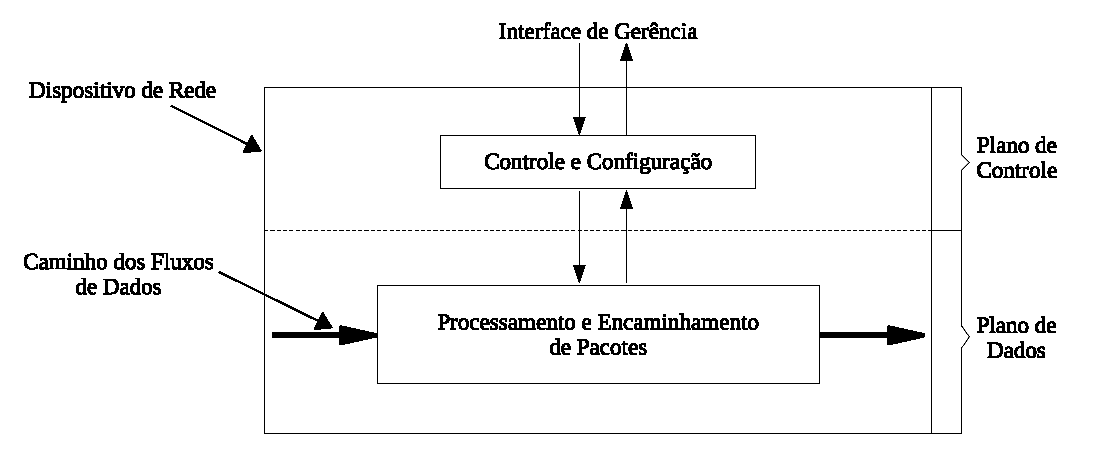
\includegraphics[width=.9\textwidth]{images/planos-introducao.eps}
  \fonte{Comer, 2013. \nocite{Comer:2013}}
  \label{fig:planos-introducao}
  
\end{figure}
\FloatBarrier

Para tentar contornar esse problema, a comunidade de pesquisa em redes de computadores tem investido em iniciativas que levem a implantação de redes com maiores recursos de programação, de forma que novas tecnologias possam ser inseridas na rede de forma gradual. Exemplos de iniciativas desse tipo são as propostas de redes ativas (\textit{active networks}) \cite{Tennenhouse:1997}, de \textit{testbeds} como o PlanetLab \cite{Chun:2003}, GENI \cite{Turner:2006} e, mais recentemente o FIBRE \cite{Salmito:2014}. Redes ativas, tiveram pouca aceitação pela necessidade de alteração dos elementos de rede para permitir que se tornassem programáveis. Iniciativas mais recentes como PlanetLab, GENI e FIBRE, apostam na adoção de recursos de virtualização para facilitar a transição para novas tecnologias. Apesar de serem consideradas de grande potencial a longo prazo, tais iniciativas ainda enfrentam desafios como garantir o desempenho exigido pelas aplicações utilizadas hoje utilizando-se tais elementos virtualizados \cite{Guedes:2006}.

Uma outra forma de abordar esse problema, consiste em estender o \textit{hardware} de encaminhamento de pacotes de forma mais restrita. Considerando-se que a operação que necessita de alto desempenho nos elementos de comutação é o encaminhamento de pacotes (plano de dados), algumas iniciativas propõem manter essa operação pouco alterada, para manter a viabilidade de desenvolvimento de hardware de alto desempenho, mas com uma possibilidade de maior controle por parte do administrador da rede. 

\gls{sdn} introduz uma perspectiva flexível para programar e manter a operacionalidade da rede  buscando desacoplar os planos de dados e de controle, desta forma, tira-se a autonomia dos equipamentos de rede que se tornam apenas encaminhadores de pacotes. Já a lógica de controle é movida para uma entidade externa, centralizada, implementada em \textit{software}. Esta, chamada de controlador, tem por funcionalidade prover a lógica de funcionamento da rede o que torna o desenvolvimento de serviços mais facilmente implementáveis, já que não há a necessidade de implementação em cada dispositivo. 

No plano de dados, o encaminhamento de pacotes, que antes era baseado em destino, passa a ser por fluxo que é definido pela combinação de campos das camadas de enlace, de rede ou de transporte, segundo o modelo TCP/IP. Dessa forma mantém-se o alto desempenho no encaminhamento de pacotes em \textit{hardware}, aliado à flexibilidade de se implementar aplicações em \textit{software}, utilizando protocolo aberto para programação da lógica do equipamento que é abstraída dos dispositivos de encaminhamento \cite{Kim:2013, Tootoonchian:2010, Rothenberg:2010}.

Pensando nisso, nasceu o OpenFlow \cite{McKeown:2008}, que por sua vez, deu origem ao conceito de \textit{Software Defined Networking}, ou redes definidas por software. A Figura \ref{fig:arch-old-sdn} apresenta um comparativo entre o modelo tradicional de rede, onde ambos os planos, de controle e de dados, são localizados em um mesmo dispositivo e o modelo \gls{sdn} que possui controle centralizado e apenas o plano de dados no dispositivo comutador.

\begin{figure}[H]
  \centering
  \caption{Modelos de rede tradicional e SDN}
  \includegraphics[width=.80\textwidth]{images/arch-old-sdn.eps}
  \fonte{Rothenberg \textit{et al.}, 2010. \nocite{Rothenberg:2010}}
  \label{fig:arch-old-sdn}
\end{figure}
\FloatBarrier

O protocolo OpenFlow é implementado em ambos os planos e dispõe de um protocolo de comunicação entre o controlador e \textit{switches}. Para garantir a confiabilidade dessa comunicação é recomendada a utilização do protocolo \gls{ssl} \cite{RFC6101} porém algumas alternativas incluem \gls{tcp}, utilizadas especialmente em redes virtuais devido à sua simplicidade, pois não necessitam de chaves criptográficas \cite{Rothenberg:2010}.

OpenFlow explora a existência de tabelas de fluxo (\textit{flow tables}) em dispositivos \textit{Ethernet} modernos. Essas tabelas são alimentadas em tempo de execução e utilizadas para implementar \textit{firewalls} \cite{Oppliger:1997}, \gls{nat} \cite{RFC3022}, \gls{qos} \cite{Aurrecoechea:1998} e coleta de estatísticas. Normalmente são proprietárias mas há um conjunto de funções que são comuns na maioria dos dispositivos. Com isso, uma forma padrão de manipulação das tabelas de fluxo pode ser implementada, independente de fornecedor. Desta maneira, OpenFlow fornece um padrão para manipulação das tabelas de fluxo, permitindo assim a partição do tráfego, o agrupamento ou isolamento da rede e o processamento ou controle do fluxo de dados, da forma desejada com base no fluxo \cite{Kontesidou:2009}.

Os principais componentes de uma arquitetura \gls{sdn} são:
\begin{itemize}
    \item Comutadores (\textit{switches}) \textit{OpenFlow};
    \item Controlador; e
    \item Protocolo de comunicação.
\end{itemize}
Estes componentes podem fazer uso do protocolo OpenFlow e/ou de outros protocolos. Por ser o primeiro e também o mais utilizado, o protocolo OpenFlow é utilizado neste trabalho como padrão de comunicação entre os dispositivos.

%=====================================================================

\subsection{Comutadores}
\label{subsec:comutador}

É o elemento responsável pelo encaminhamento dos pacotes pela rede. Pode ser específico para OpenFlow, ou ter suporte ao mesmo. No comutador (\textit{switch}) OpenFlow é mantida uma tabela de fluxo (\textit{flow table}) que armazena informações sobre como os pacotes serão processados, estatísticas, prioridades e tempo limite para novos fluxos. Além disso, cada regra é composta por um conjunto de campos do cabeçalho do pacote que podem ser visualizadas na Figura \ref{fig:flow-table}, assim como as informações de ações e estatísticas.

\begin{figure}[H]
  \centering
  \caption{Tabela de fluxo}
  \includegraphics[width=.65\textwidth]{images/flow-table.eps}
  \label{fig:flow-table}
  \fonte{Adaptado de Costa, 2014 \nocite{Costa:2004}}
\end{figure}
\FloatBarrier
%Copiado e artigo 6, reescrever
Quando um pacote chega a um equipamento com OpenFlow habilitado, os cabeçalhos do pacote são comparados (\textit{match}) às regras das entradas das tabelas de fluxos, os contadores são atualizados e as ações correspondentes são realizadas. Se não houver correspondência  (\textit{table miss}) entre o pacote e alguma entrada da tabela de fluxos, o pacote é encaminhado, por completo, ao controlador. Alternativamente, apenas o cabeçalho é encaminhado ao controlador mantendo o pacote armazenado no \textit{buffer} do \textit{hardware}. A Figura \ref{fig:fluxo-tmp} ilustra, através de um diagrama simplificado, o tratamento recebido por pacotes em um \textit{switch} OpenFlow.

Os pacotes que chegam ao controlador normalmente correspondem ao primeiro pacote de um novo fluxo ou, em função do tipo de pacote e da aplicação, o controlador pode decidir por instalar uma regra no \textit{switch} para que todos os pacotes de determinado fluxo sejam enviados para o controlador para serem tratados individualmente. Esse último caso corresponde, em geral, a pacotes de controle  (\gls{icmp} \cite{RFC0792}, \gls{dns} \cite{RFC7719}, \gls{dhcp} \cite{RFC2131}) ou de protocolos de roteamento  (\gls{ospf} \cite{RFC2328}, \gls{bgp} \cite{RFC4271}).
Todos os pacotes de uma mesma faixa de endereços \gls{ip}, ou uma conexão \gls{tcp} em determinada porta são considerados fluxos.

\begin{figure}[H]
  \centering
  \caption{Diagrama simplificado do tratamento de um pacote no \textit{switch} OpenFlow}
  \includegraphics[width=.80\textwidth]{images/flow.eps}
  \label{fig:fluxo-tmp}
  \fonte{Elaborado pelo autor a partir da especificação OpenFlow\\\cite{OpenFlowSpec:2014}}
\end{figure}
\FloatBarrier

A cada pacote recebido, é realizada a atualização dos contadores na tabela de fluxo.
Esses contadores são usados para geração de estatísticas, de maneira a monitorar o número de pacotes e bytes de cada fluxo, além do tempo de duração desde o seu início. O Quadro \ref{tab:contadores} apresenta alguns dos contadores disponíveis na tabela de fluxo. Com o auxílio deste podem ser implementados recursos de monitoramento e segurança do tráfego na rede.

\begin{table}[H]
  \centering
  %\captionof{figure}[tab:contadores]{Contadores da tabela de fluxo}
  \caption{Contadores da tabela de encaminhamento}
  \begin{tabular}{|l|c|} \hline
	\textbf{Contator} & \textbf{Tamanho em bits} \\ \hline
	\multicolumn{2}{|c|}{Por Tabela} \\ \hline
	Número de entradas Ativas & 32 \\ \hline
	Número de pacotes pesquisados & 64 \\ \hline
	Número de pacotes encontrados na tabela & 64 \\ \hline
	\multicolumn{2}{|c|}{Por fluxo} \\ \hline
	Número de pacotes recebidos & 64 \\ \hline
	Número de bytes recebidos & 64 \\ \hline
	Duração (segundos) & 32 \\ \hline
	Duração (nano segundos) & 32 \\ \hline
	\multicolumn{2}{|c|}{Por porta} \\ \hline
	Número de pacotes recebidos & 64 \\ \hline
	Número de pacotes transmitidos & 64 \\ \hline
	Número de bytes recebidos & 64 \\ \hline
	Número de bytes transmitidos & 64 \\ \hline
	Número de pacotes perdidos no recebimento & 64 \\ \hline
	Número de pacotes perdidos na transmissão & 64 \\ \hline
	Número de erros recebidos & 64 \\ \hline
  \end{tabular}
  \label{tab:contadores}
  \fonte{Elaborado pelo autor a partir da especificação OpenFlow\\  \cite{OpenFlowSpec:2014}}
\end{table}

Neste projeto o comutador a ser utilizado é o Open vSwitch \cite{website:ovs}, um \textit{switch} virtual com suporte a OpenFlow. Este comutador é projetado para permitir a automatização de grandes redes através da extensão programática, suportando ainda interfaces e protocolos de gerenciamento como, por exemplo, NetFlow \cite{rfc3954}, sFlow \cite{rfc3176} e IPFIX \cite{rfc5153}. Além disso, pode suportar a distribuição através de múltiplos servidores físicos \cite{website:ovs}.
%=====================================================================

\subsection{Controlador}
\label{subsec:controlador}

O controlador, como já citado, é o \textit{software} responsável por tomar decisões e adicionar e remover as entradas na tabela de encaminhamento, de acordo com o objetivo desejado. Exerce a função de uma camada de abstração da infraestrutura física, facilitando a criação de aplicações e serviços que gerenciem as entradas de fluxos na rede. Esse modelo assemelha-se a outros sistemas de \textit{software} que proveem abstração do \textit{hardware} e funcionalidade reutilizável. Dessa forma, o controlador atua como um \gls{so} para gerenciamento e controle das redes, e oferece uma plataforma com base na reutilização de componentes e na definição de níveis de abstração. Contudo, novas aplicações de rede podem ser desenvolvidas rapidamente \cite{Gude:2008}.

O controlador fornece uma interface para criar, modificar e controlar o fluxo de tabelas do comutador. É executado normalmente em um servidor conectado à rede e pode ser um para todos os comutadores da rede, um para cada comutador ou um para um conjunto de comutadores.  Portanto, a funcionalidade da rede de controle pode ser completamente ou localmente centralizada dependendo de como o gerenciamento dos comutadores é realizada. A exigência, no entanto, é que, se houver mais do que um controlador de processos, eles devem ter a mesma visão da topologia da rede, em qualquer momento dado. A visão de rede inclui a topologia a nível de \textit{switch}, as localizações dos usuários, \textit{hosts}, \textit{middleboxes} e outros elementos de rede e serviços. Além disso inclui todas as ligações entre os nomes e endereços.

O controlador é parte integrante de uma arquitetura de rede \gls{sdn} e para que sua comunicação com \textit{switches} OpenFlow ocorra, o controlador deve ter suporte ao mesmo. Atualmente, existem várias implementações controlador disponíveis que implementam o protocolo OpenFlow, entre os principais não comerciais estão \cite{Kreutz:2013,Xia:2015}:

\begin{itemize}
    \item \textbf{NOX} - Desenvolvido em C++, foi o primeiro controlador OpenFlow \cite{Gude:2008}. Porém não foi fortemente utilizado por causa de deficiências na sua implementação e na documentação.
    \item \textbf{POX} - Sucessor do NOX, foi desenvolvido como uma alternativa mais amigável e tem sido implementado por um grande número de engenheiros e programadores \gls{sdn}. Comparando com NOX, POX tem um ambiente de desenvolvimento mais fácil de trabalhar com uma API razoavelmente bem escrita e documentada. Também fornece uma interface Web e é escrito em Python \cite{website:pox}.
    \item \textbf{Beacon} - É um controlador SDN bem escrito e organizado. Escrito em Java, Beacon foi o primeiro controlador com o qual iniciantes pudessem trabalhar e criar um ambiente \gls{sdn}, no entanto, era limitado à topologias de rede estrela \cite{Erickson:2013}.
    \item \textbf{Floodlight} - Uma ramificação do Beacon. Enquanto que seu início tenha sido baseado no Beacon este foi desenvolvido utilizando Apache Ant, uma ferramenta popular para compilação e construção de \textit{software}, o que tornou o desenvolvimento do Floodlight mais fácil e flexível. Floodlight possui uma comunidade ativa e um grande número de recursos que podem ser adicionados ao sistema. Possui interface baseada em java e baseada em Web, além de possuir uma Interface de Programação de Aplicações (\gls{api}) \gls{rest} ou, em português, Transferência de Estado Representacional \cite{website:floodlight}.
    \item \textbf{OpenDayLight} - É um projeto colaborativo da Linux Fundation e tem sido altamente suportado por empresas como Cisco e Big Switch. Desenvolvido em Java, também inclui \gls{api} \gls{rest} e interface web. Possui suporte à \gls{sdn}, \gls{nv} , ou Virtualização de redes \cite{Chowdhury:2009} e \gls{nfv}, ou Virtualização da Funções da Rede \cite{Hawilo:2014}. Além disso, possui um grande número de módulos que podem ser utilizados para atender aos requisitos de uma organização \cite{website:odl}.
    \item \textbf{Ryu NOS} - É um \textit{framework} de \gls{sdn} baseado em componentes. O Ryu fornece componentes de software com \glspl{api} bem definidas que tornam mais fácil para os desenvolvedores criar novas aplicações de gerenciamento e controle de rede. O Ryu suporta vários protocolos para gerenciar dispositivos de rede, como OpenFlow, Netconf, OF-config, etc. Sobre o OpenFlow, o Ryu suporta totalmente as extensões 1.0, 1.2, 1.3, 1.4, 1.5 e Nicira. Todo o código está disponível gratuitamente sob a licença Apache 2.0 \cite{website:ryu}.
\end{itemize}

%=====================================================================

\subsection{Protocolo OpenFlow}
\label{subsec:protocolo-comunicacao}

O protocolo de comunicação entre os dois planos é realizado por três tipos de mensagens: controlador para o \textit{switch}, assíncrona e simétricas. 

Mensagens do tipo controlador para \textit{switch} são mensagens que o controlador envia para obter informações sobre o estado do \textit{switch}, como por exemplo verificar estatísticas de um determinado fluxo \cite{OpenFlowSpec:2014}. Essas mensagens podem ser:
%Rescrever
\begin{itemize}
    \item \textit{\textbf{Features}}: ao estabelecer uma conexão, o controlador envia esta mensagem requisitando que o \textit{switch} informe suas capacidades.
    \item \textit{\textbf{Configuration}}: o controlador envia parâmetros de configuração para os \textit{switches}. 
    \item \textit{\textbf{Modify-State}}: utilizado pelo controlador para gerenciar o estado dos \textit{switches}, deletar ou modificar regras na tabela de fluxos.
    \item \textit{\textbf{Read-State}}: utilizado pelo controlador para coletar estatísticas das tabelas de fluxos do \textit{switch}.
    \item \textit{\textbf{Packet-Out}}: utilizada pelo controlador para enviar pacotes por uma porta específica.
    \item \textit{\textbf{Barrier}}: utilizada para verificar se as dependências das mensagens foram alcançadas ou receber notificação sobre tarefas concluídas.
     \item \textit{\textbf{Role Request}}: mensagens usadas pelo controlador para configurar seu canal OpenFlow.
\end{itemize}

Mensagens assíncronas são enviadas pelo \textit{switch} sem a solicitação do controlador. \textit{Switches} enviam mensagens assíncronas para os controladores para denotar uma chegada de pacotes ou mudança de estado \cite{OpenFlowSpec:2014}. Os principais tipos de mensagens assíncronas são descritas abaixo.
\begin{itemize}
    \item \textit{\textbf{Packet-In}}: enviado pelo \textit{switch} quando há uma ação explícita na tabela de fluxos para que seja enviado para o controlador ou quando não há um \textit{match} para o pacote.
    \item \textit{\textbf{Flow-Removed}}: informa o controlador sobre a remoção de regras no \textit{switch}.
    \item \textit{\textbf{Port Status}}: informa o controlador sobre uma mudança em alguma porta.
    \item \textit{\textbf{Role Status}}: \textit{switch} informa o controlador sobre a alterações em suas regras.
    \item \textit{\textbf{Controller Status}}: \textit{switch} informa o controlador sobre a mudança em um canal OpenFlow.
    \item \textit{\textbf{Flow-monitor}}: informa o controlador sobre uma mudança na tabela de fluxo.
\end{itemize}

Finalmente, mensagens simétricas são iniciadas tanto pelo controlador como pelo \textit{switch} sem nenhuma solicitação, por exemplo o início de conexão entre controlador e \textit{switch} \cite{OpenFlowSpec:2014}. Essas mensagens são:
\begin{itemize}
    \item \textit{\textbf{Hello}}: esta mensagem é utilizada no início da conexão entre \textit{switch} e controlador.
    \item \textit{\textbf{Echo}}: utilizado para obter informações sobre a conexão entre \textit{switch} e controlador como:
latência, largura de banda e conectividade.
    \item \textit{\textbf{Error}}:  o \textit{switch} pode enviar mensagens para notificar problemas ao controlador por mensagens de erro.
    \item \textit{\textbf{Experimenter}}: na versão 1.5.0 do protocolo OpenFlow, esta mensagem é utilizada para adicionar funcionalidades experimentais.
\end{itemize}

Cada mensagem é enviada encapsulada em um pacote definido pelo protocolo OpenFlow e que é representado na Figura \ref{fig:openflow-message}.

\begin{figure}[H]
  \centering
  \caption{Formato da mensagem OpenFlow}
  \includegraphics[width=.80\textwidth]{images/openflow-message.eps}
  \label{fig:openflow-message}
  \fonte{\centering
  Elaborado pelo autor a partir de informações da especificação OpenFlow.}
\end{figure}
\FloatBarrier

O campo \textit{version} indica a versão do protocolo que está sendo utilizada. Já o  \textit{type}, indica o tipo de mensagem que está sendo enviada. O campo \textit{length} informa o tamanho da mensagem enquanto que \textit{xid} representa o ID de transação associado à mensagem. Por último, o campo \textit{payload} representa o corpo da mensagem, é neste campo onde são adicionados os diferentes tipos de mensagens apresentados anteriormente.
\section{Virtualização}
\label{sec:virtualizacao}
%Rescrever

O conceito de virtualização de redes define uma infraestrutura de redes de computadores virtuais. São definidos por \textit{software}, executando sobre máquinas físicas, de forma que toda infraestrutura virtual seja isolada da infraestrutura física, não interferindo na mesma. 

Um dos \textit{softwares} mais usados na criação de redes virtuais em nível de \textit{software} é o Xen \cite{Fernandes:2011}. Esse programa é usado na criação de máquinas virtuais em computadores pessoais e servidores, e oferece a opção de criar roteadores virtuais que podem ser utilizados na interligação de máquinas virtuais para a formação de uma rede. Em \gls{sdn} a construção de redes virtuais acontece em nível de \textit{hardware}, através da separação do tráfego da rede física em \textit{slices}, porções de fluxo do tráfego total. O FlowVisor \cite{Sherwood:2009} possibilita virtualização em \gls{sdn}.

O uso de virtualização de redes possibilita execução de experimentos distintos, sobre a mesma infraestrutura, em paralelo, sem interferência entre experimentos. Virtualização de redes também pode ser usada para isolamento de serviços. Assim, uma organização pode oferecer diversos serviços, com cada serviços executando em uma rede virtual diferente \cite{wu:2010, Mattos:2012}.

\section{Emulador Mininet}
\label{sec:mininet}

Mininet \cite{Handigol:2012} é um emulador de rede para prototipação em \gls{sdn}. A razão pela sua utilização deve-se ao fato de apenas alguns dispositivos de rede estarem disponíveis para \gls{sdn}, uma vez que ainda não é uma tecnologia difundida a nível industrial.  Além disso, a implementação de rede com elevado número de dispositivos de rede é muito difícil e dispendioso. Por isso, para contornar estes problemas, a virtualização foi realizada com a finalidade de prototipar e emular este tipo de tecnologia de rede e um dos mais importantes é o Mininet \cite{Wendong:2012}.  Mininet tem a capacidade de emular diferentes tipos de elementos de rede, tais como: \textit{host}, \textit{switches} (camada de enlace), roteadores (camada de rede) e conexões. Ele funciona em um único núcleo de Linux\cite{Negus:2015} e utiliza virtualização com a finalidade de emular uma rede completa que utiliza apenas um único sistema. No entanto, o \textit{host}, roteadores e links criados são elementos do mundo real, embora eles sejam criados por meio de software \cite{website:mininet}.

Criar uma rede no Mininet é relativamente simples. Pode-se usar linha de comando ou um componente chamado \textit{miniedit.py}, que implementa uma interface gráfica para o Mininet, este porém, possui algumas limitações em relação à linha de comando. Pela linha de comando, ao chamar o Mininet são passados os parâmetros sobre as características da rede como: topologia, número de \textit{hosts}, \textit{switches}, taxa de perda de pacotes, largura de banda, tipo de controlador, entre outros. O \textit{switch} padrão é o OpenSwitch \cite{Pettit:2010}, um \textit{switch} virtual desenvolvido especialmente para trabalhar com o protocolo Openflow. Para estudo mais aprofundado, recomenda-se a leitura da sua documentação em \cite{website:mininet}.
\section{Segurança em redes}
\label{sec:seguranca}

A segurança no nível de rede indica uma área de pesquisa muito importante, já que os usuários estão continuamente colocando seus dados em ambientes em nuvem e mais dados são transferidos através de grandes distâncias. A razão para esta evolução é a crescente popularidade dos serviços em nuvem, bem como a simplicidade e rápida capacidade dos recursos sob demanda. Os impactos variam de acordo com os tipos de ameaças, e como defesa são criados diversos sistemas de segurança que agem como barreira de proteção, como por exemplo, \textit{firewalls}. Os principais tipos de ameaças serão estudadas a seguir. Também é apresentado um estudo mais detalhado do ataque do tipo varredura, foco deste trabalho.

\subsection{Tipos de ameaças}
Dos diversos tipos de ameaças que podem ocorrer nas redes de computadores, destacam-se algumas que são notórias por causar frequentes transtornos aos usuário, tais como:

\textbf{Fraude}:
Segundo Houaiss, Villar e Francisco (2001)\nocite{Houaiss:2001}, é "qualquer ato ardiloso, enganoso, de má-fé, com intuito de lesar ou ludibriar outrem, ou de não cumprir determinado dever; logro". Esta categoria engloba as notificações de tentativas de fraudes, ou seja, de incidentes em que ocorre uma tentativa de obter vantagem, sejam por meios como correios eletrônicos não solicitados em massa (\textit{spam}) e páginas falsas.
    
\textbf{Ataque de negação de serviço (\textit{\gls{dos}}}:
Um ataque de negação de serviço busca sobrecarregar serviços na rede dificultando o seu uso por usuários legítimos. Esse tipo de ataque, por sua natureza, pode produzir variações no volume de tráfego que normalmente são visíveis no gráfico de fluxo. Segundo Sperotto \textit{et al.} (2010)\nocite{Sperotto:2010} no entanto, na detecção de intrusão por fluxo, é abordado implicitamente o problema de ataques \gls{dos} por força bruta, ou seja, um tipo de \gls{dos} que depende de esgotamento de recursos ou sobrecarga da rede. Infelizmente, é quase impossível de detectar diretamente ataques \gls{dos} semânticas.
    
\textbf{Infestações viróticas automatizadas (\textit{Worms})}:
São pequenos programas de computador criados para causar danos na máquina infectada e se auto replica pela rede, tirando cópias de si em cada computador \cite{Sperotto:2010}.
    
\textbf{Exército de máquinas controladas sem autorização (\textit{Botnets})}:
Grupo de computadores comprometidos, chamados de computadores zumbis que são controlados remotamente por um centro de controle. \textit{Botnets} são muito utilizados para lançamento de ataques  como \textit{spams}, DoS e \textit{worms} \cite{Sperotto:2010}.
    
\textbf{Varredura de portas maliciosa (\textit{port scans})}:
Técnica utilizada para encontrar fraquezas de um computador ou de uma rede. Enquanto esta técnica não é um ataque real, os hackers a usam para detectar quais portas estão abertas em um computador. Baseado nas informações sobre portas abertas, o acesso não autorizado pode ser obtido.

Os métodos citados também podem também ser utilizados em conjunto, como por exemplo a utilização de \textit{botnets} que, controlados remotamente, podem efetuar ataques DoS a um mesmo servidor e ao mesmo tempo. A esse tipo de ataque é dado o nome de Negação de Serviço Distribuída (\gls{ddos})

Do ponto de vista de segurança, existe uma quantidade crescente de incidência de ataques de negação de serviço, \gls{dos}, durante os últimos anos \cite{Seeber:2015}. Além disso, segundo a \gls{cert.br}, responsável por tratar incidentes de segurança e computadores que envolvam redes conectadas à Internet brasileira, foram reportados 722.205 incidências de segurança somente no ano de 2015, sendo mais da metade (53\%), ataques do tipo \textit{port scan}.

\subsection{Técnicas de varredura}
\label{sec:varredura}

Um dos tipos mais comuns de ataques, a varredura consiste no envio de diversos tipos de pacotes com o intuito de se conhecer mais sobre o nó alvo ou a rede em questão. Através das respostas obtidas para esses pacotes, o atacante é capaz de chegar a diversas informações que possam ajudar em futuros ataques de diversos tipos. Alguns tipos de informações que podem ser descobertas incluem (não somente): A atividade dos servidores, informações relativas a softwares utilizados no sistema, informações sobre o \textit{firewall} e topologia da rede.

Uma das principais dificuldades nas soluções desse tipo de ataque é que as varreduras são consideradas atividades legais, e ocorrem na Internet de forma rotineira, inclusive com fins não maliciosos.

Antes de explorar as técnicas de varredura, faz-se necessário o entendimento de alguns conceitos de comunicação \gls{tcp}. Para obter um serviço \gls{tcp}, uma conexão necessita ser efetivada entre os computadores origem e destino. Esta conexão é realizada através dos chamados \textit{sockets}, formados pelo par endereço \gls{ip} e número de porta, de ambos, computador de origem e computador de destino. Entre estes dois \textit{sockets} ocorre a transferência de segmentos.

Um segmento consiste em um cabeçalho \gls{tcp} seguido, opcionalmente, por informação. Um cabeçalho \gls{tcp} pode possuir seis \textit{flags} que podem ser ativadas ou desativadas ao mesmo tempo \cite{Comer:2013}, são elas:

\begin{itemize}
    \item \textbf{SYN} - \textit{bit} de sincronismo, é o \textit{bit} que informa que este é um dos dois primeiros segmentos de estabelecimento da conexão.
    \item \textbf{ACK} - \textit{bit} de reconhecimento, indica que o valor do campo de reconhecimento está carregando um reconhecimento válido.
    \item \textbf{PSH} - \textit{bit} de \textit{push}, este mecanismo, que pode ser acionado pela aplicação, informa ao \gls{tcp} origem e destino que a aplicação solicita a transmissão rápida dos dados enviados, mesmo que ela contenha um número baixo de \textit{bytes}, não preenchendo o tamanho mínimo do \textit{buffer} de transmissão.
    \item \textbf{RST} - \textit{bit} de \textit{reset}, informa o destino que a conexão foi abortada neste sentido pela origem
    \item \textbf{FIN} - \textit{bit} de terminação, indica que este pacote é um dos pacotes de finalização da conexão.
\end{itemize}

Em uma comunicação \gls{tcp}, uma conexão deve ser estabelecida entre os dois pontos (\textit{sockets}) para que a transferência de dados ocorra.
Inicialmente a máquina emissora, também chamada de cliente, transmite um segmento cuja \textit{flag} SYN é de 1 (para assinalar que se trata de um segmento de sincronização), com um número de ordem X, que se chama número de ordem inicial do cliente.

A seguir, a máquina receptora, chamada de servidor, recebe o segmento inicial que provém do cliente e envia-lhe um aviso de recepção, isto é, um segmento cuja \textit{flag} ACK é de 1 e a \textit{flag} SYN é de 1 (porque ainda se trata de uma sincronização). Este segmento contém o número de ordem do servidor, que é o número de ordem inicial do cliente. O campo mais importante deste segmento é o campo de aviso de recepção, que contém o número de ordem inicial do cliente, incrementado de 1.

Por último, o cliente transmite ao servidor um aviso de recepção, ou seja, um segmento cuja \textit{flag} ACK é de 1, cuja \textit{flag} SYN é de zero (não se trata mais de um segmento de sincronização). O seu número de ordem é incrementado e o número de aviso de recepção representa o número de ordem inicial do servidor, incrementado de 1.

Depois dessa sequência de trocas (Figura \ref{fig:troca-tcp}), também chamada de \textit{handshake}, ou, aperto de mãos em português, as duas máquinas estão conectadas e a comunicação pode ser efetivada.

\begin{figure}[H]
  \centering
  \caption{Estabelecimento de conexão TCP}
  \includegraphics[width=0.5\textwidth]{images/conexao-tcp.eps}
  \label{fig:troca-tcp}
   \fonte{Elaborado pelo autor.}
\end{figure}
\FloatBarrier

Os passos a seguir são definidos pela RFC 793 \cite{rfc793}, utilizada pela grande maioria das implementações \gls{tcp} e exploradas em técnicas de varredura.

\begin{itemize}
    \item Quando um segmento SYN chega em um aporta aberta, é continuado o procedimento de \textit{handshake} como discutido anteriormente; 
    \item Quando um segmento SYN (ou FIN) chega em uma porta fechada, o segmento é descartado e um segmento RST é retornado para o cliente;
    \item Quanto um segmento FIN chega em uma porta que esteja aberta, o segmento é descartado.
    \item Quando um segmento RST chega em uma porta que esteja ouvindo (aberta), o segmento é descartado;
    \item Quando um segmento RST chega em uma porta que não esteja ouvindo (fechada), o segmento é descartado;
    \item Quando um segmento ACK chega à uma porta aberta, o mesmo é descartado e retornado um segmento RST.
\end{itemize}


Devido à sua natureza, \textit{scans} podem facilmente criar um vasto número diferente de fluxos. Segundo Speroto \textit{et al.} (2010)\nocite{Sperotto:2010}, há três categorias de varredura, são elas:
\begin{itemize}
    \item \textbf{\textit{scan} horizontal} - quando um \textit{host} de origem varre uma porta especifica em diferentes \textit{hosts} alvo;
    \item \textbf{\textit{scan} vertical} - quando um \textit{host} de origem verifica várias portas distintas de um mesmo \textit{host} alvo; e
    \item \textbf{\textit{scan} misto} - quando há a combinação das varreduras vertical e horizontal.
\end{itemize}

Existem várias técnicas de varredura de porta disponíveis e podem facilmente ser automatizadas por ferramentas como Nmap \cite{Lyon:2009}. Alguns métodos utilizados para varredura são estudados a seguir \cite{deVivo:1999, Christopher:2001}.
\begin{itemize}
\item \textbf{\textit{TCP Connect}} - É a forma mais comum de \textit{scanning}. Basicamente uma conexão TCP regular (\textit{handshake} completo) para cada porta definida na varredura. Para cada porta, a conexão pode resultar em sucesso, indicando uma porta aberta ou em falha caso contrário. Essa técnica é facilmente implementada pois não necessita de privilégios especiais e, do mesmo modo, é facilmente detectável. Através de \textit{logs} do sistema alvo é possível verificar mensagens de requisição de conexão e de erro para as conexões negadas. Neste método, o \textit{scanner} envia uma mensagem SYN para o sistema alvo. Se uma porta estiver (aberta) ouvindo com um serviço, a conexão se sucederá. Um SYN é retornado estabelecendo o número de sequência inicial. Um ACK considera o campo numérico de confirmação válido. Se a porta estiver (fechada) sem serviço ouvindo, uma mensagem RST é retornada, para reiniciar o pedido de conexão. Alguns exemplos de \textit{scanners} podem ser Nmap, Amap e Blaster. %Exemplo de \textit{scanner}: nmap.

\item \textbf{TCP SYN} - Também conhecida por \textit{Half Open} por não explorar um \textit{handshake} completo. Nesta técnica o \textit{scanner} envia uma mensagem SYN, como se estivesse pedindo uma conexão. Se responder como um RST, indica que a porta está fechada, e uma nova porta é testada. Se a resposta da máquina alvo for um SYN/ACK, indica que a porta se encontra ouvindo. O \textit{scanner} envia então um RST cancelando o \textit{handshake}. A vantagem desse tipo de \textit{scanning} é o fato de, mesmo ainda podendo ser detectado, tentativas de conexões SYN são menos frequentemente registradas se comparadas com conexões \gls{tcp} completas. %Exemplos de \textit{scanners}: amap, hping2, netstat, nmap.

\item \textbf{Exploração FIN} - Neste método, quando um segmento FIN é enviado para uma porta fechada, o computador alvo responde com um TCP RST. Quando a porta estiver aberta, o segmento é ignorado e o computador alvo não responde. O \textit{scanner} não recebe nunhuma resposta, pois não podem pertencer a uma conexão estabelecida. %Exemplos de \textit{scanners}: hping2, nmap.

\item \textbf{Xmas Tree} - é uma variação do método TCP FIN, neste, são utilizadas mensagens com prioridade TCP FIN/URG/PSH. Quando estiver ouvindo, o \textit{host} alvo não responde, caso contrário, responde com um TCP RST. %Exemplos de \textit{scanners}: hping2, netstat, nmap.

\item \textbf{TCP Null (sem flags ativos)} - também é uma variação do método TCP FIN, neste, tem-se resposta para portas fechadas, mas não para portas abertas.% Exemplos de \textit{scanners}: hping2, netstat, nmap.

\item \textbf{Varredura ACK} - Técnica utilizada para identificar \textit{firewalls}. Um segmento ACK que não pertença a nenhum conexão é gerado pelo \textit{scanner}. Se um RST é devolvido pela máquina alvo, tanto em uma porta aberta como em uma fechada, as portas são classificadas como não tendo \textit{firewall}.

\item \textbf{Varredura ARP} - Não se trata exatamente de varredura de portas mas essa técnica é utilizada para descobrir dispositivos ativos na rede local, para depois realizar a varredura de portas somente nos computadores ativos. O \textit{scanner} envia uma série de pacotes de protocolo \gls{arp} \cite{RFC0826} e incrementa o valor do \gls{ip} alvo a cada \textit{broadcast}.
\end{itemize}


\subsection{Ferramentas de Varredura}

Para que as varreduras sejam efetuadas, tem-se a possibilidade de utilizar ferramentas que possibilite a varredura utilizando as diferentes formas citadas na seção anterior. Uma das ferramentas mais utilizadas, e que foi utilizada neste trabalho é o Nmap \cite{Lyon:2009}.

O Nmap é um \textit{software} que oferece uma gama muito grande de recursos e funcionalidades, como detecção do Sistema Operacional remoto, o serviço e a versão que está em uso no host, o exame de ociosidade por identificação (ID) de Internet Protocol (IP), o rápido exame de multiportas por ping entre tantas outras. Possui versões para plataformas Unix, Windows, e MacOS sendo utilizado tanto por interface console como também em interface gráfica, o software Nmap é um utilitário livre e de código aberto, usado para exploração de redes, segurança e auditoria, capaz de examinar grandes redes ou simplesmente um único host.
A função principal do Nmap é realizar uma varredura em portas \gls{tcp} e o retorno dessa varredura é classificado em um dos seguintes estados: aberta, fechada, filtrada, nao filtrada e a combinação de aberta/filtrada ou fechada/filtrada \cite{Lyon:2009}. Vários outros softwares que são utilizados para gerencia e controle de redes de computadores fazem uso do Nmap pois pode ser usado diretamente, sempre que se desejar uma verificação de portas em um \textit{host} que esteja em uma rede local ou na Internet.
O uso mais simples do Nmap é escanear diretamente uma máquina da rede, onde uma quantidade enorme de portas \gls{tcp} será examinada na máquina alvo, e cada porta será classificada de acordo com seu estado.
Na linha de comando do Nmap, tudo que não for uma opção ou argumento de opção será tratado como uma especificação de hospedeiro alvo. O caso mais simples é a especificação de um endereço IP ou nome de hospedeiro alvo para exame \cite{Lyon:2009}.


\subsection{Sistemas de detecção e prevenção de intrusão}

O isolamento da rede em redes virtuais permite uma maior segurança devido ao seu isolamento, porém problemas tradicionais relacionados à segurança continuam existindo em ambientes virtualizados pois 60\% a 70\% dos ataques à segurança da rede são de origem interna segundo Lynch (2006)\nocite{Lynch:2006}. Uma das formas de se proteger desses ataques é monitorar o tráfego em busca de atividades maliciosas ou violação de políticas. Para realizar o monitoramento de pacotes na rede, a solução mais apropriada é o sistema de detecção de intrusão, que realiza o monitoramento passivo dos pacotes na rede. Porém, esse tipo de análise não permite que sejam tomadas ações para prevenir tais ataques, e então faz se necessário um sistema de prevenção de intrusão para bloquear esses pacotes.

Segundo Kruegel (2004)\nocite{Kruegel:2004}, "Detecção de intrusão é o processo de identificar e responder à atividades maliciosas na computação e redes de dados". Uma tentativa de intrusão, também chamada de ataque, refere-se a uma série de ações em que um intruso tenta obter o ganho do sistema e o objetivo de um \gls{ids} é discriminar tentativas de intrusão e preparação de intrusão do uso normal do sistema.

Em redes tradicionais, para detectar e prevenir intrusos maliciosos na rede de dados, administradores normalmente necessitam implantar diversos detectores de intrusão em diferentes locais da rede, e então analisar dados do tráfego coletados localmente ou em um nodo centralizado. Infelizmente, arquiteturas \gls{ids}/\gls{ips} utilizadas atualmente possuem muitas barreiras para gerir nós distribuídos. Em primeiro lugar, os nós de detecção de intrusão devem suportar diferentes configurações. Como as configurações dependem da topologia da rede, configurações manuais e mudanças frequentes são inevitáveis para tornar a política em nós distribuídos eficaz e coerente. Em segundo lugar, algoritmos de detecção de intrusão eficazes normalmente são desenhados para um determinado tipo de ataque. Para desenvolver sistemas de detecção eficazes, mais e mais protocolos de proteção são criados, o que resulta na redução do desempenho da rede. Além disso, dispositivos de rede normalmente possuem protocolos proprietários, o que torna mais difícil desenvolver interfaces de gerenciamento automáticas \cite{Wang:2015}.

Vários trabalhos para \gls{ids} tem sido desenvolvidos desde o início de sua pesquisa nos anos 1980. Essas propostas podem ser classificadas de acordo com várias características, como tipo de dados analisado (\textit{logs} ou dados do pacote), tipo de análise (em tempo real ou \textit{offline}) ou pelo tipo de processamento (centralizado ou distribuído). No entanto, os modelos de classificação mais conhecidos são os baseados em assinatura e os baseados em anomalia \cite{Axelsson:2000}.

Sistemas de detecção de intrusão baseados em assinatura realizam a detecção através da comparação de dados do pacote com uma base de dados conhecida. O \gls{ids} Snort \cite{Roesch:1999} é um dos exemplos mais utilizados dessa técnica, verificando padrões de pacote através da análise de dados da carga útil (\textit{payload}) do pacote. O Snortik \cite{Fagundes16} também é um bom exemplo, neste, é proposto uma integração entre o \gls{ids} Snort e o sistema de \textit{firewall} do sistema MikroTik RouteOS \cite{mikrotik16} com a finalidade de automatizar o processo de reação à ataques. \glspl{ids} baseados em assinatura possuem alta precisão, raramente apresentando alarmes para fluxos normais, porém, não reconhecem fluxos novos, não presentes na sua base de dados. Além disso, a inspeção de pacotes é difícil e até mesmo impossível de ser realizada  em redes com taxas com múltiplos Gigabits por segundo \cite{Lai:2004, Gao:2006}.

Sistemas de detecção de intrusão baseados em anomalia por sua vez, comparam dados recebidos com um "modelo de normalidade" que descreve o comportamento normal da rede. Alterações significativas desse modelo são consideradas como anomalias. Exemplos de criação de comportamentos podem ser redes neurais, técnicas de análise de estatísticas e teoria das probabilidades. A principal vantagem desse tipo de detecção é o fato de também detectar fluxos não conhecidos anteriormente \cite{Owezarski:2010}. No entanto, podem existir casos em que fluxos podem ser diferentes da normalidade esperada mas não necessariamente serem maliciosos resultando em alarmes falsos positivos.

Um \gls{ids} deve ser capaz de lidar com o número crescente do tráfego e ataques na rede. No entanto, alternativas baseadas nas análise de carga útil possuem eficácia em redes entre 100Mbps e 200Mbps \cite{Lai:2004, Gao:2006} podendo chegar a 1Gbps quando hardware dedicado é empregado \cite{Vasiliadis:2008}. Sistemas como Bro \cite{Paxson:1999} e Snort \cite{Roesch:1999} apresentam alto consumo de recursos  quando confrontado com a enorme quantidade de dados de alta taxa de transferência encontrados atualmente \cite{Dreger:2004}. Além disso, protocolos criptografados podem representar um desafio a mais para sistemas de carga útil. Para redes de alta taxas de transmissão, alternativas à inspeção de pacotes são muito importantes. Uma dessas alternativas e que tem atraído pesquisadores é a detecção de intrusão de anomalias baseada em fluxo.

Com esta abordagem, são analisados os padrões de comunicação dentro da rede, ao invés do conteúdo dos pacotes individuais. Hoje em dia os sistemas de medição especiais são capazes de fornecer, para cada par de endereços IP e números de porta, informações agregadas, como a quantidade de bytes transferidos, o número de pacotes enviados e o tempo que determinado fluxo de dados esteve ativo. Essas informações podem então ser exportadas para outros sistemas analisarem, para então, serem usados para detectar intrusões \cite{Sperotto:2010}.

Considerando essa inflexibilidade sobre os equipamentos atuais, os interesses sobre abstrair funções de rede de \textit{switches} dedicados para aplicações \gls{sdn} vem aumentando. Sendo assim, as políticas de segurança podem ser instaladas pelo controlador como regras nas tabelas de fluxo \cite{Kim:2013}, em vez de configurações manuais e independentes. Com isso, o \textit{switch} provê apenas a função de filtro de acordo com a regra na tabela de fluxo, não influenciando significativamente no desempenho da rede. Além disso, \gls{sdn} tem recursos naturais de estatísticas que são úteis para a análise de detecção de intrusão, de modo que o controlador obtém mais visibilidade sobre o tráfego da rede. Portanto, \gls{sdn} parece fornecer uma arquitetura mais adequada para \gls{ips}.



\chapter{Fundamentação Teórica}
\label{cap:fundamentacao}

Neste capítulo serão apresentados tópicos relacionados ao presente trabalho que se fazem necessários para o entendimento deste Trabalho de Conclusão. O capítulo está organizado da seguinte forma: na Seção \ref{sec:sdn-openflow} são abordados os conceitos sobre \gls{sdn} e Openflow; na Seção \ref{sec:virtualizacao} é feita uma abordagem referente a virtualização de redes; na Seção \ref{sec:mininet} é abordado o software de simulação de rede Mininet, utilizado para realização de testes neste trabalho; e por fim, na Seção \ref{sec:seguranca}, é discutido o assunto de segurança em redes de computadores, os principais tipos de ataques e soluções além da ferramenta utilizada para varredura de portas.

\section{Redes Definidas por Software}
\label{sec:sdn-openflow}

As redes de computadores se tornaram parte da infraestrutura crítica de empresas, escolas e residências, tendo crescido bastante desde a sua origem. O sucesso das redes de computadores se deve, em grande parte, à simplicidade de seu núcleo. Na arquitetura atual, a inteligência está localizada nos sistemas de borda, enquanto que o núcleo é simples e transparente. Embora essa simplicidade tenha tido sucesso, também é razão para o seu engessamento, pois apresenta limitações estruturais que são difíceis de serem resolvidas, tais como escalabilidade, mobilidade e gerenciamento de serviço \cite{Clarkl:2004}.

Por causa desta expansão, o trabalho dos pesquisadores da área tornou-se muito mais importante, porém mesmo com o grande número de equipamentos e protocolos criados para suportar essa expansão, ainda tem-se uma grande barreira. A maioria das ideias que surgem não conseguem ser testadas por falta de maneiras práticas que possibilitem a realização de experimentos com novos protocolos em uma rede realista, para que possa obter a confiança necessária para uma implantação em escala global \cite{McKeown:2008}. 

Como apresentado por Kreutz \cite{Kreutz:2014}, redes de computadores podem ser separadas em três planos: de controle, de dados e de gerência. Entende-se por plano de controle a porção da rede que abriga os \textit{softwares} responsáveis por ditar o comportamento da rede. Decisões de roteamento, \textit{firewall}, priorização de pacotes são de responsabilidade do plano de controle. O plano de dados é o que executa o encaminhamento dos pacotes com base nas regras ditadas pelo plano de controle. Já o plano de gerência inclui serviços utilizados para monitorar a rede e configurar remotamente o plano de controle utilizando protocolos como \gls{snmp} \cite{RFC1157}. 

Em síntese, o plano de gerência define as regras da rede, o de controle implementa essas regras e o plano de dados realiza o encaminhamento de pacotes de acordo com as regras impostas pelo plano de controle. Em redes \gls{ip} tradicionais, os planos de controle e dados são acoplados em um mesmo hardware, como pode ser visualizado na Figura \ref{fig:planos-introducao}, tornando a arquitetura de rede complexa e por consequência dificulta a sua configuração e o seu gerenciamento.


\begin{figure}[H]
  \centering
  \caption{Planos de redes de computadores.}
  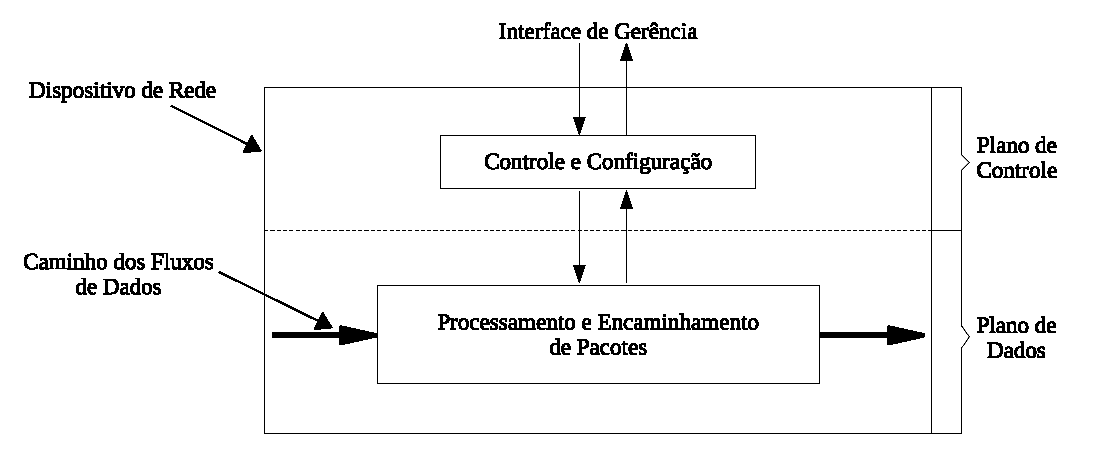
\includegraphics[width=.9\textwidth]{images/planos-introducao.eps}
  \fonte{Comer, 2013. \nocite{Comer:2013}}
  \label{fig:planos-introducao}
  
\end{figure}
\FloatBarrier

Para tentar contornar esse problema, a comunidade de pesquisa em redes de computadores tem investido em iniciativas que levem a implantação de redes com maiores recursos de programação, de forma que novas tecnologias possam ser inseridas na rede de forma gradual. Exemplos de iniciativas desse tipo são as propostas de redes ativas (\textit{active networks}) \cite{Tennenhouse:1997}, de \textit{testbeds} como o PlanetLab \cite{Chun:2003}, GENI \cite{Turner:2006} e, mais recentemente o FIBRE \cite{Salmito:2014}. Redes ativas, tiveram pouca aceitação pela necessidade de alteração dos elementos de rede para permitir que se tornassem programáveis. Iniciativas mais recentes como PlanetLab, GENI e FIBRE, apostam na adoção de recursos de virtualização para facilitar a transição para novas tecnologias. Apesar de serem consideradas de grande potencial a longo prazo, tais iniciativas ainda enfrentam desafios como garantir o desempenho exigido pelas aplicações utilizadas hoje utilizando-se tais elementos virtualizados \cite{Guedes:2006}.

Uma outra forma de abordar esse problema, consiste em estender o \textit{hardware} de encaminhamento de pacotes de forma mais restrita. Considerando-se que a operação que necessita de alto desempenho nos elementos de comutação é o encaminhamento de pacotes (plano de dados), algumas iniciativas propõem manter essa operação pouco alterada, para manter a viabilidade de desenvolvimento de hardware de alto desempenho, mas com uma possibilidade de maior controle por parte do administrador da rede. 

\gls{sdn} introduz uma perspectiva flexível para programar e manter a operacionalidade da rede  buscando desacoplar os planos de dados e de controle, desta forma, tira-se a autonomia dos equipamentos de rede que se tornam apenas encaminhadores de pacotes. Já a lógica de controle é movida para uma entidade externa, centralizada, implementada em \textit{software}. Esta, chamada de controlador, tem por funcionalidade prover a lógica de funcionamento da rede o que torna o desenvolvimento de serviços mais facilmente implementáveis, já que não há a necessidade de implementação em cada dispositivo. 

No plano de dados, o encaminhamento de pacotes, que antes era baseado em destino, passa a ser por fluxo que é definido pela combinação de campos das camadas de enlace, de rede ou de transporte, segundo o modelo TCP/IP. Dessa forma mantém-se o alto desempenho no encaminhamento de pacotes em \textit{hardware}, aliado à flexibilidade de se implementar aplicações em \textit{software}, utilizando protocolo aberto para programação da lógica do equipamento que é abstraída dos dispositivos de encaminhamento \cite{Kim:2013, Tootoonchian:2010, Rothenberg:2010}.

Pensando nisso, nasceu o OpenFlow \cite{McKeown:2008}, que por sua vez, deu origem ao conceito de \textit{Software Defined Networking}, ou redes definidas por software. A Figura \ref{fig:arch-old-sdn} apresenta um comparativo entre o modelo tradicional de rede, onde ambos os planos, de controle e de dados, são localizados em um mesmo dispositivo e o modelo \gls{sdn} que possui controle centralizado e apenas o plano de dados no dispositivo comutador.

\begin{figure}[H]
  \centering
  \caption{Modelos de rede tradicional e SDN}
  \includegraphics[width=.80\textwidth]{images/arch-old-sdn.eps}
  \fonte{Rothenberg \textit{et al.}, 2010. \nocite{Rothenberg:2010}}
  \label{fig:arch-old-sdn}
\end{figure}
\FloatBarrier

O protocolo OpenFlow é implementado em ambos os planos e dispõe de um protocolo de comunicação entre o controlador e \textit{switches}. Para garantir a confiabilidade dessa comunicação é recomendada a utilização do protocolo \gls{ssl} \cite{RFC6101} porém algumas alternativas incluem \gls{tcp}, utilizadas especialmente em redes virtuais devido à sua simplicidade, pois não necessitam de chaves criptográficas \cite{Rothenberg:2010}.

OpenFlow explora a existência de tabelas de fluxo (\textit{flow tables}) em dispositivos \textit{Ethernet} modernos. Essas tabelas são alimentadas em tempo de execução e utilizadas para implementar \textit{firewalls} \cite{Oppliger:1997}, \gls{nat} \cite{RFC3022}, \gls{qos} \cite{Aurrecoechea:1998} e coleta de estatísticas. Normalmente são proprietárias mas há um conjunto de funções que são comuns na maioria dos dispositivos. Com isso, uma forma padrão de manipulação das tabelas de fluxo pode ser implementada, independente de fornecedor. Desta maneira, OpenFlow fornece um padrão para manipulação das tabelas de fluxo, permitindo assim a partição do tráfego, o agrupamento ou isolamento da rede e o processamento ou controle do fluxo de dados, da forma desejada com base no fluxo \cite{Kontesidou:2009}.

Os principais componentes de uma arquitetura \gls{sdn} são:
\begin{itemize}
    \item Comutadores (\textit{switches}) \textit{OpenFlow};
    \item Controlador; e
    \item Protocolo de comunicação.
\end{itemize}
Estes componentes podem fazer uso do protocolo OpenFlow e/ou de outros protocolos. Por ser o primeiro e também o mais utilizado, o protocolo OpenFlow é utilizado neste trabalho como padrão de comunicação entre os dispositivos.

%=====================================================================

\subsection{Comutadores}
\label{subsec:comutador}

É o elemento responsável pelo encaminhamento dos pacotes pela rede. Pode ser específico para OpenFlow, ou ter suporte ao mesmo. No comutador (\textit{switch}) OpenFlow é mantida uma tabela de fluxo (\textit{flow table}) que armazena informações sobre como os pacotes serão processados, estatísticas, prioridades e tempo limite para novos fluxos. Além disso, cada regra é composta por um conjunto de campos do cabeçalho do pacote que podem ser visualizadas na Figura \ref{fig:flow-table}, assim como as informações de ações e estatísticas.

\begin{figure}[H]
  \centering
  \caption{Tabela de fluxo}
  \includegraphics[width=.65\textwidth]{images/flow-table.eps}
  \label{fig:flow-table}
  \fonte{Adaptado de Costa, 2014 \nocite{Costa:2004}}
\end{figure}
\FloatBarrier
%Copiado e artigo 6, reescrever
Quando um pacote chega a um equipamento com OpenFlow habilitado, os cabeçalhos do pacote são comparados (\textit{match}) às regras das entradas das tabelas de fluxos, os contadores são atualizados e as ações correspondentes são realizadas. Se não houver correspondência  (\textit{table miss}) entre o pacote e alguma entrada da tabela de fluxos, o pacote é encaminhado, por completo, ao controlador. Alternativamente, apenas o cabeçalho é encaminhado ao controlador mantendo o pacote armazenado no \textit{buffer} do \textit{hardware}. A Figura \ref{fig:fluxo-tmp} ilustra, através de um diagrama simplificado, o tratamento recebido por pacotes em um \textit{switch} OpenFlow.

Os pacotes que chegam ao controlador normalmente correspondem ao primeiro pacote de um novo fluxo ou, em função do tipo de pacote e da aplicação, o controlador pode decidir por instalar uma regra no \textit{switch} para que todos os pacotes de determinado fluxo sejam enviados para o controlador para serem tratados individualmente. Esse último caso corresponde, em geral, a pacotes de controle  (\gls{icmp} \cite{RFC0792}, \gls{dns} \cite{RFC7719}, \gls{dhcp} \cite{RFC2131}) ou de protocolos de roteamento  (\gls{ospf} \cite{RFC2328}, \gls{bgp} \cite{RFC4271}).
Todos os pacotes de uma mesma faixa de endereços \gls{ip}, ou uma conexão \gls{tcp} em determinada porta são considerados fluxos.

\begin{figure}[H]
  \centering
  \caption{Diagrama simplificado do tratamento de um pacote no \textit{switch} OpenFlow}
  \includegraphics[width=.80\textwidth]{images/flow.eps}
  \label{fig:fluxo-tmp}
  \fonte{Elaborado pelo autor a partir da especificação OpenFlow\\\cite{OpenFlowSpec:2014}}
\end{figure}
\FloatBarrier

A cada pacote recebido, é realizada a atualização dos contadores na tabela de fluxo.
Esses contadores são usados para geração de estatísticas, de maneira a monitorar o número de pacotes e bytes de cada fluxo, além do tempo de duração desde o seu início. O Quadro \ref{tab:contadores} apresenta alguns dos contadores disponíveis na tabela de fluxo. Com o auxílio deste podem ser implementados recursos de monitoramento e segurança do tráfego na rede.

\begin{table}[H]
  \centering
  %\captionof{figure}[tab:contadores]{Contadores da tabela de fluxo}
  \caption{Contadores da tabela de encaminhamento}
  \begin{tabular}{|l|c|} \hline
	\textbf{Contator} & \textbf{Tamanho em bits} \\ \hline
	\multicolumn{2}{|c|}{Por Tabela} \\ \hline
	Número de entradas Ativas & 32 \\ \hline
	Número de pacotes pesquisados & 64 \\ \hline
	Número de pacotes encontrados na tabela & 64 \\ \hline
	\multicolumn{2}{|c|}{Por fluxo} \\ \hline
	Número de pacotes recebidos & 64 \\ \hline
	Número de bytes recebidos & 64 \\ \hline
	Duração (segundos) & 32 \\ \hline
	Duração (nano segundos) & 32 \\ \hline
	\multicolumn{2}{|c|}{Por porta} \\ \hline
	Número de pacotes recebidos & 64 \\ \hline
	Número de pacotes transmitidos & 64 \\ \hline
	Número de bytes recebidos & 64 \\ \hline
	Número de bytes transmitidos & 64 \\ \hline
	Número de pacotes perdidos no recebimento & 64 \\ \hline
	Número de pacotes perdidos na transmissão & 64 \\ \hline
	Número de erros recebidos & 64 \\ \hline
  \end{tabular}
  \label{tab:contadores}
  \fonte{Elaborado pelo autor a partir da especificação OpenFlow\\  \cite{OpenFlowSpec:2014}}
\end{table}

Neste projeto o comutador a ser utilizado é o Open vSwitch \cite{website:ovs}, um \textit{switch} virtual com suporte a OpenFlow. Este comutador é projetado para permitir a automatização de grandes redes através da extensão programática, suportando ainda interfaces e protocolos de gerenciamento como, por exemplo, NetFlow \cite{rfc3954}, sFlow \cite{rfc3176} e IPFIX \cite{rfc5153}. Além disso, pode suportar a distribuição através de múltiplos servidores físicos \cite{website:ovs}.
%=====================================================================

\subsection{Controlador}
\label{subsec:controlador}

O controlador, como já citado, é o \textit{software} responsável por tomar decisões e adicionar e remover as entradas na tabela de encaminhamento, de acordo com o objetivo desejado. Exerce a função de uma camada de abstração da infraestrutura física, facilitando a criação de aplicações e serviços que gerenciem as entradas de fluxos na rede. Esse modelo assemelha-se a outros sistemas de \textit{software} que proveem abstração do \textit{hardware} e funcionalidade reutilizável. Dessa forma, o controlador atua como um \gls{so} para gerenciamento e controle das redes, e oferece uma plataforma com base na reutilização de componentes e na definição de níveis de abstração. Contudo, novas aplicações de rede podem ser desenvolvidas rapidamente \cite{Gude:2008}.

O controlador fornece uma interface para criar, modificar e controlar o fluxo de tabelas do comutador. É executado normalmente em um servidor conectado à rede e pode ser um para todos os comutadores da rede, um para cada comutador ou um para um conjunto de comutadores.  Portanto, a funcionalidade da rede de controle pode ser completamente ou localmente centralizada dependendo de como o gerenciamento dos comutadores é realizada. A exigência, no entanto, é que, se houver mais do que um controlador de processos, eles devem ter a mesma visão da topologia da rede, em qualquer momento dado. A visão de rede inclui a topologia a nível de \textit{switch}, as localizações dos usuários, \textit{hosts}, \textit{middleboxes} e outros elementos de rede e serviços. Além disso inclui todas as ligações entre os nomes e endereços.

O controlador é parte integrante de uma arquitetura de rede \gls{sdn} e para que sua comunicação com \textit{switches} OpenFlow ocorra, o controlador deve ter suporte ao mesmo. Atualmente, existem várias implementações controlador disponíveis que implementam o protocolo OpenFlow, entre os principais não comerciais estão \cite{Kreutz:2013,Xia:2015}:

\begin{itemize}
    \item \textbf{NOX} - Desenvolvido em C++, foi o primeiro controlador OpenFlow \cite{Gude:2008}. Porém não foi fortemente utilizado por causa de deficiências na sua implementação e na documentação.
    \item \textbf{POX} - Sucessor do NOX, foi desenvolvido como uma alternativa mais amigável e tem sido implementado por um grande número de engenheiros e programadores \gls{sdn}. Comparando com NOX, POX tem um ambiente de desenvolvimento mais fácil de trabalhar com uma API razoavelmente bem escrita e documentada. Também fornece uma interface Web e é escrito em Python \cite{website:pox}.
    \item \textbf{Beacon} - É um controlador SDN bem escrito e organizado. Escrito em Java, Beacon foi o primeiro controlador com o qual iniciantes pudessem trabalhar e criar um ambiente \gls{sdn}, no entanto, era limitado à topologias de rede estrela \cite{Erickson:2013}.
    \item \textbf{Floodlight} - Uma ramificação do Beacon. Enquanto que seu início tenha sido baseado no Beacon este foi desenvolvido utilizando Apache Ant, uma ferramenta popular para compilação e construção de \textit{software}, o que tornou o desenvolvimento do Floodlight mais fácil e flexível. Floodlight possui uma comunidade ativa e um grande número de recursos que podem ser adicionados ao sistema. Possui interface baseada em java e baseada em Web, além de possuir uma Interface de Programação de Aplicações (\gls{api}) \gls{rest} ou, em português, Transferência de Estado Representacional \cite{website:floodlight}.
    \item \textbf{OpenDayLight} - É um projeto colaborativo da Linux Fundation e tem sido altamente suportado por empresas como Cisco e Big Switch. Desenvolvido em Java, também inclui \gls{api} \gls{rest} e interface web. Possui suporte à \gls{sdn}, \gls{nv} , ou Virtualização de redes \cite{Chowdhury:2009} e \gls{nfv}, ou Virtualização da Funções da Rede \cite{Hawilo:2014}. Além disso, possui um grande número de módulos que podem ser utilizados para atender aos requisitos de uma organização \cite{website:odl}.
    \item \textbf{Ryu NOS} - É um \textit{framework} de \gls{sdn} baseado em componentes. O Ryu fornece componentes de software com \glspl{api} bem definidas que tornam mais fácil para os desenvolvedores criar novas aplicações de gerenciamento e controle de rede. O Ryu suporta vários protocolos para gerenciar dispositivos de rede, como OpenFlow, Netconf, OF-config, etc. Sobre o OpenFlow, o Ryu suporta totalmente as extensões 1.0, 1.2, 1.3, 1.4, 1.5 e Nicira. Todo o código está disponível gratuitamente sob a licença Apache 2.0 \cite{website:ryu}.
\end{itemize}

%=====================================================================

\subsection{Protocolo OpenFlow}
\label{subsec:protocolo-comunicacao}

O protocolo de comunicação entre os dois planos é realizado por três tipos de mensagens: controlador para o \textit{switch}, assíncrona e simétricas. 

Mensagens do tipo controlador para \textit{switch} são mensagens que o controlador envia para obter informações sobre o estado do \textit{switch}, como por exemplo verificar estatísticas de um determinado fluxo \cite{OpenFlowSpec:2014}. Essas mensagens podem ser:
%Rescrever
\begin{itemize}
    \item \textit{\textbf{Features}}: ao estabelecer uma conexão, o controlador envia esta mensagem requisitando que o \textit{switch} informe suas capacidades.
    \item \textit{\textbf{Configuration}}: o controlador envia parâmetros de configuração para os \textit{switches}. 
    \item \textit{\textbf{Modify-State}}: utilizado pelo controlador para gerenciar o estado dos \textit{switches}, deletar ou modificar regras na tabela de fluxos.
    \item \textit{\textbf{Read-State}}: utilizado pelo controlador para coletar estatísticas das tabelas de fluxos do \textit{switch}.
    \item \textit{\textbf{Packet-Out}}: utilizada pelo controlador para enviar pacotes por uma porta específica.
    \item \textit{\textbf{Barrier}}: utilizada para verificar se as dependências das mensagens foram alcançadas ou receber notificação sobre tarefas concluídas.
     \item \textit{\textbf{Role Request}}: mensagens usadas pelo controlador para configurar seu canal OpenFlow.
\end{itemize}

Mensagens assíncronas são enviadas pelo \textit{switch} sem a solicitação do controlador. \textit{Switches} enviam mensagens assíncronas para os controladores para denotar uma chegada de pacotes ou mudança de estado \cite{OpenFlowSpec:2014}. Os principais tipos de mensagens assíncronas são descritas abaixo.
\begin{itemize}
    \item \textit{\textbf{Packet-In}}: enviado pelo \textit{switch} quando há uma ação explícita na tabela de fluxos para que seja enviado para o controlador ou quando não há um \textit{match} para o pacote.
    \item \textit{\textbf{Flow-Removed}}: informa o controlador sobre a remoção de regras no \textit{switch}.
    \item \textit{\textbf{Port Status}}: informa o controlador sobre uma mudança em alguma porta.
    \item \textit{\textbf{Role Status}}: \textit{switch} informa o controlador sobre a alterações em suas regras.
    \item \textit{\textbf{Controller Status}}: \textit{switch} informa o controlador sobre a mudança em um canal OpenFlow.
    \item \textit{\textbf{Flow-monitor}}: informa o controlador sobre uma mudança na tabela de fluxo.
\end{itemize}

Finalmente, mensagens simétricas são iniciadas tanto pelo controlador como pelo \textit{switch} sem nenhuma solicitação, por exemplo o início de conexão entre controlador e \textit{switch} \cite{OpenFlowSpec:2014}. Essas mensagens são:
\begin{itemize}
    \item \textit{\textbf{Hello}}: esta mensagem é utilizada no início da conexão entre \textit{switch} e controlador.
    \item \textit{\textbf{Echo}}: utilizado para obter informações sobre a conexão entre \textit{switch} e controlador como:
latência, largura de banda e conectividade.
    \item \textit{\textbf{Error}}:  o \textit{switch} pode enviar mensagens para notificar problemas ao controlador por mensagens de erro.
    \item \textit{\textbf{Experimenter}}: na versão 1.5.0 do protocolo OpenFlow, esta mensagem é utilizada para adicionar funcionalidades experimentais.
\end{itemize}

Cada mensagem é enviada encapsulada em um pacote definido pelo protocolo OpenFlow e que é representado na Figura \ref{fig:openflow-message}.

\begin{figure}[H]
  \centering
  \caption{Formato da mensagem OpenFlow}
  \includegraphics[width=.80\textwidth]{images/openflow-message.eps}
  \label{fig:openflow-message}
  \fonte{\centering
  Elaborado pelo autor a partir de informações da especificação OpenFlow.}
\end{figure}
\FloatBarrier

O campo \textit{version} indica a versão do protocolo que está sendo utilizada. Já o  \textit{type}, indica o tipo de mensagem que está sendo enviada. O campo \textit{length} informa o tamanho da mensagem enquanto que \textit{xid} representa o ID de transação associado à mensagem. Por último, o campo \textit{payload} representa o corpo da mensagem, é neste campo onde são adicionados os diferentes tipos de mensagens apresentados anteriormente.
\section{Virtualização}
\label{sec:virtualizacao}
%Rescrever

O conceito de virtualização de redes define uma infraestrutura de redes de computadores virtuais. São definidos por \textit{software}, executando sobre máquinas físicas, de forma que toda infraestrutura virtual seja isolada da infraestrutura física, não interferindo na mesma. 

Um dos \textit{softwares} mais usados na criação de redes virtuais em nível de \textit{software} é o Xen \cite{Fernandes:2011}. Esse programa é usado na criação de máquinas virtuais em computadores pessoais e servidores, e oferece a opção de criar roteadores virtuais que podem ser utilizados na interligação de máquinas virtuais para a formação de uma rede. Em \gls{sdn} a construção de redes virtuais acontece em nível de \textit{hardware}, através da separação do tráfego da rede física em \textit{slices}, porções de fluxo do tráfego total. O FlowVisor \cite{Sherwood:2009} possibilita virtualização em \gls{sdn}.

O uso de virtualização de redes possibilita execução de experimentos distintos, sobre a mesma infraestrutura, em paralelo, sem interferência entre experimentos. Virtualização de redes também pode ser usada para isolamento de serviços. Assim, uma organização pode oferecer diversos serviços, com cada serviços executando em uma rede virtual diferente \cite{wu:2010, Mattos:2012}.

\section{Emulador Mininet}
\label{sec:mininet}

Mininet \cite{Handigol:2012} é um emulador de rede para prototipação em \gls{sdn}. A razão pela sua utilização deve-se ao fato de apenas alguns dispositivos de rede estarem disponíveis para \gls{sdn}, uma vez que ainda não é uma tecnologia difundida a nível industrial.  Além disso, a implementação de rede com elevado número de dispositivos de rede é muito difícil e dispendioso. Por isso, para contornar estes problemas, a virtualização foi realizada com a finalidade de prototipar e emular este tipo de tecnologia de rede e um dos mais importantes é o Mininet \cite{Wendong:2012}.  Mininet tem a capacidade de emular diferentes tipos de elementos de rede, tais como: \textit{host}, \textit{switches} (camada de enlace), roteadores (camada de rede) e conexões. Ele funciona em um único núcleo de Linux\cite{Negus:2015} e utiliza virtualização com a finalidade de emular uma rede completa que utiliza apenas um único sistema. No entanto, o \textit{host}, roteadores e links criados são elementos do mundo real, embora eles sejam criados por meio de software \cite{website:mininet}.

Criar uma rede no Mininet é relativamente simples. Pode-se usar linha de comando ou um componente chamado \textit{miniedit.py}, que implementa uma interface gráfica para o Mininet, este porém, possui algumas limitações em relação à linha de comando. Pela linha de comando, ao chamar o Mininet são passados os parâmetros sobre as características da rede como: topologia, número de \textit{hosts}, \textit{switches}, taxa de perda de pacotes, largura de banda, tipo de controlador, entre outros. O \textit{switch} padrão é o OpenSwitch \cite{Pettit:2010}, um \textit{switch} virtual desenvolvido especialmente para trabalhar com o protocolo Openflow. Para estudo mais aprofundado, recomenda-se a leitura da sua documentação em \cite{website:mininet}.
\section{Segurança em redes}
\label{sec:seguranca}

A segurança no nível de rede indica uma área de pesquisa muito importante, já que os usuários estão continuamente colocando seus dados em ambientes em nuvem e mais dados são transferidos através de grandes distâncias. A razão para esta evolução é a crescente popularidade dos serviços em nuvem, bem como a simplicidade e rápida capacidade dos recursos sob demanda. Os impactos variam de acordo com os tipos de ameaças, e como defesa são criados diversos sistemas de segurança que agem como barreira de proteção, como por exemplo, \textit{firewalls}. Os principais tipos de ameaças serão estudadas a seguir. Também é apresentado um estudo mais detalhado do ataque do tipo varredura, foco deste trabalho.

\subsection{Tipos de ameaças}
Dos diversos tipos de ameaças que podem ocorrer nas redes de computadores, destacam-se algumas que são notórias por causar frequentes transtornos aos usuário, tais como:

\textbf{Fraude}:
Segundo Houaiss, Villar e Francisco (2001)\nocite{Houaiss:2001}, é "qualquer ato ardiloso, enganoso, de má-fé, com intuito de lesar ou ludibriar outrem, ou de não cumprir determinado dever; logro". Esta categoria engloba as notificações de tentativas de fraudes, ou seja, de incidentes em que ocorre uma tentativa de obter vantagem, sejam por meios como correios eletrônicos não solicitados em massa (\textit{spam}) e páginas falsas.
    
\textbf{Ataque de negação de serviço (\textit{\gls{dos}}}:
Um ataque de negação de serviço busca sobrecarregar serviços na rede dificultando o seu uso por usuários legítimos. Esse tipo de ataque, por sua natureza, pode produzir variações no volume de tráfego que normalmente são visíveis no gráfico de fluxo. Segundo Sperotto \textit{et al.} (2010)\nocite{Sperotto:2010} no entanto, na detecção de intrusão por fluxo, é abordado implicitamente o problema de ataques \gls{dos} por força bruta, ou seja, um tipo de \gls{dos} que depende de esgotamento de recursos ou sobrecarga da rede. Infelizmente, é quase impossível de detectar diretamente ataques \gls{dos} semânticas.
    
\textbf{Infestações viróticas automatizadas (\textit{Worms})}:
São pequenos programas de computador criados para causar danos na máquina infectada e se auto replica pela rede, tirando cópias de si em cada computador \cite{Sperotto:2010}.
    
\textbf{Exército de máquinas controladas sem autorização (\textit{Botnets})}:
Grupo de computadores comprometidos, chamados de computadores zumbis que são controlados remotamente por um centro de controle. \textit{Botnets} são muito utilizados para lançamento de ataques  como \textit{spams}, DoS e \textit{worms} \cite{Sperotto:2010}.
    
\textbf{Varredura de portas maliciosa (\textit{port scans})}:
Técnica utilizada para encontrar fraquezas de um computador ou de uma rede. Enquanto esta técnica não é um ataque real, os hackers a usam para detectar quais portas estão abertas em um computador. Baseado nas informações sobre portas abertas, o acesso não autorizado pode ser obtido.

Os métodos citados também podem também ser utilizados em conjunto, como por exemplo a utilização de \textit{botnets} que, controlados remotamente, podem efetuar ataques DoS a um mesmo servidor e ao mesmo tempo. A esse tipo de ataque é dado o nome de Negação de Serviço Distribuída (\gls{ddos})

Do ponto de vista de segurança, existe uma quantidade crescente de incidência de ataques de negação de serviço, \gls{dos}, durante os últimos anos \cite{Seeber:2015}. Além disso, segundo a \gls{cert.br}, responsável por tratar incidentes de segurança e computadores que envolvam redes conectadas à Internet brasileira, foram reportados 722.205 incidências de segurança somente no ano de 2015, sendo mais da metade (53\%), ataques do tipo \textit{port scan}.

\subsection{Técnicas de varredura}
\label{sec:varredura}

Um dos tipos mais comuns de ataques, a varredura consiste no envio de diversos tipos de pacotes com o intuito de se conhecer mais sobre o nó alvo ou a rede em questão. Através das respostas obtidas para esses pacotes, o atacante é capaz de chegar a diversas informações que possam ajudar em futuros ataques de diversos tipos. Alguns tipos de informações que podem ser descobertas incluem (não somente): A atividade dos servidores, informações relativas a softwares utilizados no sistema, informações sobre o \textit{firewall} e topologia da rede.

Uma das principais dificuldades nas soluções desse tipo de ataque é que as varreduras são consideradas atividades legais, e ocorrem na Internet de forma rotineira, inclusive com fins não maliciosos.

Antes de explorar as técnicas de varredura, faz-se necessário o entendimento de alguns conceitos de comunicação \gls{tcp}. Para obter um serviço \gls{tcp}, uma conexão necessita ser efetivada entre os computadores origem e destino. Esta conexão é realizada através dos chamados \textit{sockets}, formados pelo par endereço \gls{ip} e número de porta, de ambos, computador de origem e computador de destino. Entre estes dois \textit{sockets} ocorre a transferência de segmentos.

Um segmento consiste em um cabeçalho \gls{tcp} seguido, opcionalmente, por informação. Um cabeçalho \gls{tcp} pode possuir seis \textit{flags} que podem ser ativadas ou desativadas ao mesmo tempo \cite{Comer:2013}, são elas:

\begin{itemize}
    \item \textbf{SYN} - \textit{bit} de sincronismo, é o \textit{bit} que informa que este é um dos dois primeiros segmentos de estabelecimento da conexão.
    \item \textbf{ACK} - \textit{bit} de reconhecimento, indica que o valor do campo de reconhecimento está carregando um reconhecimento válido.
    \item \textbf{PSH} - \textit{bit} de \textit{push}, este mecanismo, que pode ser acionado pela aplicação, informa ao \gls{tcp} origem e destino que a aplicação solicita a transmissão rápida dos dados enviados, mesmo que ela contenha um número baixo de \textit{bytes}, não preenchendo o tamanho mínimo do \textit{buffer} de transmissão.
    \item \textbf{RST} - \textit{bit} de \textit{reset}, informa o destino que a conexão foi abortada neste sentido pela origem
    \item \textbf{FIN} - \textit{bit} de terminação, indica que este pacote é um dos pacotes de finalização da conexão.
\end{itemize}

Em uma comunicação \gls{tcp}, uma conexão deve ser estabelecida entre os dois pontos (\textit{sockets}) para que a transferência de dados ocorra.
Inicialmente a máquina emissora, também chamada de cliente, transmite um segmento cuja \textit{flag} SYN é de 1 (para assinalar que se trata de um segmento de sincronização), com um número de ordem X, que se chama número de ordem inicial do cliente.

A seguir, a máquina receptora, chamada de servidor, recebe o segmento inicial que provém do cliente e envia-lhe um aviso de recepção, isto é, um segmento cuja \textit{flag} ACK é de 1 e a \textit{flag} SYN é de 1 (porque ainda se trata de uma sincronização). Este segmento contém o número de ordem do servidor, que é o número de ordem inicial do cliente. O campo mais importante deste segmento é o campo de aviso de recepção, que contém o número de ordem inicial do cliente, incrementado de 1.

Por último, o cliente transmite ao servidor um aviso de recepção, ou seja, um segmento cuja \textit{flag} ACK é de 1, cuja \textit{flag} SYN é de zero (não se trata mais de um segmento de sincronização). O seu número de ordem é incrementado e o número de aviso de recepção representa o número de ordem inicial do servidor, incrementado de 1.

Depois dessa sequência de trocas (Figura \ref{fig:troca-tcp}), também chamada de \textit{handshake}, ou, aperto de mãos em português, as duas máquinas estão conectadas e a comunicação pode ser efetivada.

\begin{figure}[H]
  \centering
  \caption{Estabelecimento de conexão TCP}
  \includegraphics[width=0.5\textwidth]{images/conexao-tcp.eps}
  \label{fig:troca-tcp}
   \fonte{Elaborado pelo autor.}
\end{figure}
\FloatBarrier

Os passos a seguir são definidos pela RFC 793 \cite{rfc793}, utilizada pela grande maioria das implementações \gls{tcp} e exploradas em técnicas de varredura.

\begin{itemize}
    \item Quando um segmento SYN chega em um aporta aberta, é continuado o procedimento de \textit{handshake} como discutido anteriormente; 
    \item Quando um segmento SYN (ou FIN) chega em uma porta fechada, o segmento é descartado e um segmento RST é retornado para o cliente;
    \item Quanto um segmento FIN chega em uma porta que esteja aberta, o segmento é descartado.
    \item Quando um segmento RST chega em uma porta que esteja ouvindo (aberta), o segmento é descartado;
    \item Quando um segmento RST chega em uma porta que não esteja ouvindo (fechada), o segmento é descartado;
    \item Quando um segmento ACK chega à uma porta aberta, o mesmo é descartado e retornado um segmento RST.
\end{itemize}


Devido à sua natureza, \textit{scans} podem facilmente criar um vasto número diferente de fluxos. Segundo Speroto \textit{et al.} (2010)\nocite{Sperotto:2010}, há três categorias de varredura, são elas:
\begin{itemize}
    \item \textbf{\textit{scan} horizontal} - quando um \textit{host} de origem varre uma porta especifica em diferentes \textit{hosts} alvo;
    \item \textbf{\textit{scan} vertical} - quando um \textit{host} de origem verifica várias portas distintas de um mesmo \textit{host} alvo; e
    \item \textbf{\textit{scan} misto} - quando há a combinação das varreduras vertical e horizontal.
\end{itemize}

Existem várias técnicas de varredura de porta disponíveis e podem facilmente ser automatizadas por ferramentas como Nmap \cite{Lyon:2009}. Alguns métodos utilizados para varredura são estudados a seguir \cite{deVivo:1999, Christopher:2001}.
\begin{itemize}
\item \textbf{\textit{TCP Connect}} - É a forma mais comum de \textit{scanning}. Basicamente uma conexão TCP regular (\textit{handshake} completo) para cada porta definida na varredura. Para cada porta, a conexão pode resultar em sucesso, indicando uma porta aberta ou em falha caso contrário. Essa técnica é facilmente implementada pois não necessita de privilégios especiais e, do mesmo modo, é facilmente detectável. Através de \textit{logs} do sistema alvo é possível verificar mensagens de requisição de conexão e de erro para as conexões negadas. Neste método, o \textit{scanner} envia uma mensagem SYN para o sistema alvo. Se uma porta estiver (aberta) ouvindo com um serviço, a conexão se sucederá. Um SYN é retornado estabelecendo o número de sequência inicial. Um ACK considera o campo numérico de confirmação válido. Se a porta estiver (fechada) sem serviço ouvindo, uma mensagem RST é retornada, para reiniciar o pedido de conexão. Alguns exemplos de \textit{scanners} podem ser Nmap, Amap e Blaster. %Exemplo de \textit{scanner}: nmap.

\item \textbf{TCP SYN} - Também conhecida por \textit{Half Open} por não explorar um \textit{handshake} completo. Nesta técnica o \textit{scanner} envia uma mensagem SYN, como se estivesse pedindo uma conexão. Se responder como um RST, indica que a porta está fechada, e uma nova porta é testada. Se a resposta da máquina alvo for um SYN/ACK, indica que a porta se encontra ouvindo. O \textit{scanner} envia então um RST cancelando o \textit{handshake}. A vantagem desse tipo de \textit{scanning} é o fato de, mesmo ainda podendo ser detectado, tentativas de conexões SYN são menos frequentemente registradas se comparadas com conexões \gls{tcp} completas. %Exemplos de \textit{scanners}: amap, hping2, netstat, nmap.

\item \textbf{Exploração FIN} - Neste método, quando um segmento FIN é enviado para uma porta fechada, o computador alvo responde com um TCP RST. Quando a porta estiver aberta, o segmento é ignorado e o computador alvo não responde. O \textit{scanner} não recebe nunhuma resposta, pois não podem pertencer a uma conexão estabelecida. %Exemplos de \textit{scanners}: hping2, nmap.

\item \textbf{Xmas Tree} - é uma variação do método TCP FIN, neste, são utilizadas mensagens com prioridade TCP FIN/URG/PSH. Quando estiver ouvindo, o \textit{host} alvo não responde, caso contrário, responde com um TCP RST. %Exemplos de \textit{scanners}: hping2, netstat, nmap.

\item \textbf{TCP Null (sem flags ativos)} - também é uma variação do método TCP FIN, neste, tem-se resposta para portas fechadas, mas não para portas abertas.% Exemplos de \textit{scanners}: hping2, netstat, nmap.

\item \textbf{Varredura ACK} - Técnica utilizada para identificar \textit{firewalls}. Um segmento ACK que não pertença a nenhum conexão é gerado pelo \textit{scanner}. Se um RST é devolvido pela máquina alvo, tanto em uma porta aberta como em uma fechada, as portas são classificadas como não tendo \textit{firewall}.

\item \textbf{Varredura ARP} - Não se trata exatamente de varredura de portas mas essa técnica é utilizada para descobrir dispositivos ativos na rede local, para depois realizar a varredura de portas somente nos computadores ativos. O \textit{scanner} envia uma série de pacotes de protocolo \gls{arp} \cite{RFC0826} e incrementa o valor do \gls{ip} alvo a cada \textit{broadcast}.
\end{itemize}


\subsection{Ferramentas de Varredura}

Para que as varreduras sejam efetuadas, tem-se a possibilidade de utilizar ferramentas que possibilite a varredura utilizando as diferentes formas citadas na seção anterior. Uma das ferramentas mais utilizadas, e que foi utilizada neste trabalho é o Nmap \cite{Lyon:2009}.

O Nmap é um \textit{software} que oferece uma gama muito grande de recursos e funcionalidades, como detecção do Sistema Operacional remoto, o serviço e a versão que está em uso no host, o exame de ociosidade por identificação (ID) de Internet Protocol (IP), o rápido exame de multiportas por ping entre tantas outras. Possui versões para plataformas Unix, Windows, e MacOS sendo utilizado tanto por interface console como também em interface gráfica, o software Nmap é um utilitário livre e de código aberto, usado para exploração de redes, segurança e auditoria, capaz de examinar grandes redes ou simplesmente um único host.
A função principal do Nmap é realizar uma varredura em portas \gls{tcp} e o retorno dessa varredura é classificado em um dos seguintes estados: aberta, fechada, filtrada, nao filtrada e a combinação de aberta/filtrada ou fechada/filtrada \cite{Lyon:2009}. Vários outros softwares que são utilizados para gerencia e controle de redes de computadores fazem uso do Nmap pois pode ser usado diretamente, sempre que se desejar uma verificação de portas em um \textit{host} que esteja em uma rede local ou na Internet.
O uso mais simples do Nmap é escanear diretamente uma máquina da rede, onde uma quantidade enorme de portas \gls{tcp} será examinada na máquina alvo, e cada porta será classificada de acordo com seu estado.
Na linha de comando do Nmap, tudo que não for uma opção ou argumento de opção será tratado como uma especificação de hospedeiro alvo. O caso mais simples é a especificação de um endereço IP ou nome de hospedeiro alvo para exame \cite{Lyon:2009}.


\subsection{Sistemas de detecção e prevenção de intrusão}

O isolamento da rede em redes virtuais permite uma maior segurança devido ao seu isolamento, porém problemas tradicionais relacionados à segurança continuam existindo em ambientes virtualizados pois 60\% a 70\% dos ataques à segurança da rede são de origem interna segundo Lynch (2006)\nocite{Lynch:2006}. Uma das formas de se proteger desses ataques é monitorar o tráfego em busca de atividades maliciosas ou violação de políticas. Para realizar o monitoramento de pacotes na rede, a solução mais apropriada é o sistema de detecção de intrusão, que realiza o monitoramento passivo dos pacotes na rede. Porém, esse tipo de análise não permite que sejam tomadas ações para prevenir tais ataques, e então faz se necessário um sistema de prevenção de intrusão para bloquear esses pacotes.

Segundo Kruegel (2004)\nocite{Kruegel:2004}, "Detecção de intrusão é o processo de identificar e responder à atividades maliciosas na computação e redes de dados". Uma tentativa de intrusão, também chamada de ataque, refere-se a uma série de ações em que um intruso tenta obter o ganho do sistema e o objetivo de um \gls{ids} é discriminar tentativas de intrusão e preparação de intrusão do uso normal do sistema.

Em redes tradicionais, para detectar e prevenir intrusos maliciosos na rede de dados, administradores normalmente necessitam implantar diversos detectores de intrusão em diferentes locais da rede, e então analisar dados do tráfego coletados localmente ou em um nodo centralizado. Infelizmente, arquiteturas \gls{ids}/\gls{ips} utilizadas atualmente possuem muitas barreiras para gerir nós distribuídos. Em primeiro lugar, os nós de detecção de intrusão devem suportar diferentes configurações. Como as configurações dependem da topologia da rede, configurações manuais e mudanças frequentes são inevitáveis para tornar a política em nós distribuídos eficaz e coerente. Em segundo lugar, algoritmos de detecção de intrusão eficazes normalmente são desenhados para um determinado tipo de ataque. Para desenvolver sistemas de detecção eficazes, mais e mais protocolos de proteção são criados, o que resulta na redução do desempenho da rede. Além disso, dispositivos de rede normalmente possuem protocolos proprietários, o que torna mais difícil desenvolver interfaces de gerenciamento automáticas \cite{Wang:2015}.

Vários trabalhos para \gls{ids} tem sido desenvolvidos desde o início de sua pesquisa nos anos 1980. Essas propostas podem ser classificadas de acordo com várias características, como tipo de dados analisado (\textit{logs} ou dados do pacote), tipo de análise (em tempo real ou \textit{offline}) ou pelo tipo de processamento (centralizado ou distribuído). No entanto, os modelos de classificação mais conhecidos são os baseados em assinatura e os baseados em anomalia \cite{Axelsson:2000}.

Sistemas de detecção de intrusão baseados em assinatura realizam a detecção através da comparação de dados do pacote com uma base de dados conhecida. O \gls{ids} Snort \cite{Roesch:1999} é um dos exemplos mais utilizados dessa técnica, verificando padrões de pacote através da análise de dados da carga útil (\textit{payload}) do pacote. O Snortik \cite{Fagundes16} também é um bom exemplo, neste, é proposto uma integração entre o \gls{ids} Snort e o sistema de \textit{firewall} do sistema MikroTik RouteOS \cite{mikrotik16} com a finalidade de automatizar o processo de reação à ataques. \glspl{ids} baseados em assinatura possuem alta precisão, raramente apresentando alarmes para fluxos normais, porém, não reconhecem fluxos novos, não presentes na sua base de dados. Além disso, a inspeção de pacotes é difícil e até mesmo impossível de ser realizada  em redes com taxas com múltiplos Gigabits por segundo \cite{Lai:2004, Gao:2006}.

Sistemas de detecção de intrusão baseados em anomalia por sua vez, comparam dados recebidos com um "modelo de normalidade" que descreve o comportamento normal da rede. Alterações significativas desse modelo são consideradas como anomalias. Exemplos de criação de comportamentos podem ser redes neurais, técnicas de análise de estatísticas e teoria das probabilidades. A principal vantagem desse tipo de detecção é o fato de também detectar fluxos não conhecidos anteriormente \cite{Owezarski:2010}. No entanto, podem existir casos em que fluxos podem ser diferentes da normalidade esperada mas não necessariamente serem maliciosos resultando em alarmes falsos positivos.

Um \gls{ids} deve ser capaz de lidar com o número crescente do tráfego e ataques na rede. No entanto, alternativas baseadas nas análise de carga útil possuem eficácia em redes entre 100Mbps e 200Mbps \cite{Lai:2004, Gao:2006} podendo chegar a 1Gbps quando hardware dedicado é empregado \cite{Vasiliadis:2008}. Sistemas como Bro \cite{Paxson:1999} e Snort \cite{Roesch:1999} apresentam alto consumo de recursos  quando confrontado com a enorme quantidade de dados de alta taxa de transferência encontrados atualmente \cite{Dreger:2004}. Além disso, protocolos criptografados podem representar um desafio a mais para sistemas de carga útil. Para redes de alta taxas de transmissão, alternativas à inspeção de pacotes são muito importantes. Uma dessas alternativas e que tem atraído pesquisadores é a detecção de intrusão de anomalias baseada em fluxo.

Com esta abordagem, são analisados os padrões de comunicação dentro da rede, ao invés do conteúdo dos pacotes individuais. Hoje em dia os sistemas de medição especiais são capazes de fornecer, para cada par de endereços IP e números de porta, informações agregadas, como a quantidade de bytes transferidos, o número de pacotes enviados e o tempo que determinado fluxo de dados esteve ativo. Essas informações podem então ser exportadas para outros sistemas analisarem, para então, serem usados para detectar intrusões \cite{Sperotto:2010}.

Considerando essa inflexibilidade sobre os equipamentos atuais, os interesses sobre abstrair funções de rede de \textit{switches} dedicados para aplicações \gls{sdn} vem aumentando. Sendo assim, as políticas de segurança podem ser instaladas pelo controlador como regras nas tabelas de fluxo \cite{Kim:2013}, em vez de configurações manuais e independentes. Com isso, o \textit{switch} provê apenas a função de filtro de acordo com a regra na tabela de fluxo, não influenciando significativamente no desempenho da rede. Além disso, \gls{sdn} tem recursos naturais de estatísticas que são úteis para a análise de detecção de intrusão, de modo que o controlador obtém mais visibilidade sobre o tráfego da rede. Portanto, \gls{sdn} parece fornecer uma arquitetura mais adequada para \gls{ips}.



\chapter{Fundamentação Teórica}
\label{cap:fundamentacao}

Neste capítulo serão apresentados tópicos relacionados ao presente trabalho que se fazem necessários para o entendimento deste Trabalho de Conclusão. O capítulo está organizado da seguinte forma: na Seção \ref{sec:sdn-openflow} são abordados os conceitos sobre \gls{sdn} e Openflow; na Seção \ref{sec:virtualizacao} é feita uma abordagem referente a virtualização de redes; na Seção \ref{sec:mininet} é abordado o software de simulação de rede Mininet, utilizado para realização de testes neste trabalho; e por fim, na Seção \ref{sec:seguranca}, é discutido o assunto de segurança em redes de computadores, os principais tipos de ataques e soluções além da ferramenta utilizada para varredura de portas.

\section{Redes Definidas por Software}
\label{sec:sdn-openflow}

As redes de computadores se tornaram parte da infraestrutura crítica de empresas, escolas e residências, tendo crescido bastante desde a sua origem. O sucesso das redes de computadores se deve, em grande parte, à simplicidade de seu núcleo. Na arquitetura atual, a inteligência está localizada nos sistemas de borda, enquanto que o núcleo é simples e transparente. Embora essa simplicidade tenha tido sucesso, também é razão para o seu engessamento, pois apresenta limitações estruturais que são difíceis de serem resolvidas, tais como escalabilidade, mobilidade e gerenciamento de serviço \cite{Clarkl:2004}.

Por causa desta expansão, o trabalho dos pesquisadores da área tornou-se muito mais importante, porém mesmo com o grande número de equipamentos e protocolos criados para suportar essa expansão, ainda tem-se uma grande barreira. A maioria das ideias que surgem não conseguem ser testadas por falta de maneiras práticas que possibilitem a realização de experimentos com novos protocolos em uma rede realista, para que possa obter a confiança necessária para uma implantação em escala global \cite{McKeown:2008}. 

Como apresentado por Kreutz \cite{Kreutz:2014}, redes de computadores podem ser separadas em três planos: de controle, de dados e de gerência. Entende-se por plano de controle a porção da rede que abriga os \textit{softwares} responsáveis por ditar o comportamento da rede. Decisões de roteamento, \textit{firewall}, priorização de pacotes são de responsabilidade do plano de controle. O plano de dados é o que executa o encaminhamento dos pacotes com base nas regras ditadas pelo plano de controle. Já o plano de gerência inclui serviços utilizados para monitorar a rede e configurar remotamente o plano de controle utilizando protocolos como \gls{snmp} \cite{RFC1157}. 

Em síntese, o plano de gerência define as regras da rede, o de controle implementa essas regras e o plano de dados realiza o encaminhamento de pacotes de acordo com as regras impostas pelo plano de controle. Em redes \gls{ip} tradicionais, os planos de controle e dados são acoplados em um mesmo hardware, como pode ser visualizado na Figura \ref{fig:planos-introducao}, tornando a arquitetura de rede complexa e por consequência dificulta a sua configuração e o seu gerenciamento.


\begin{figure}[H]
  \centering
  \caption{Planos de redes de computadores.}
  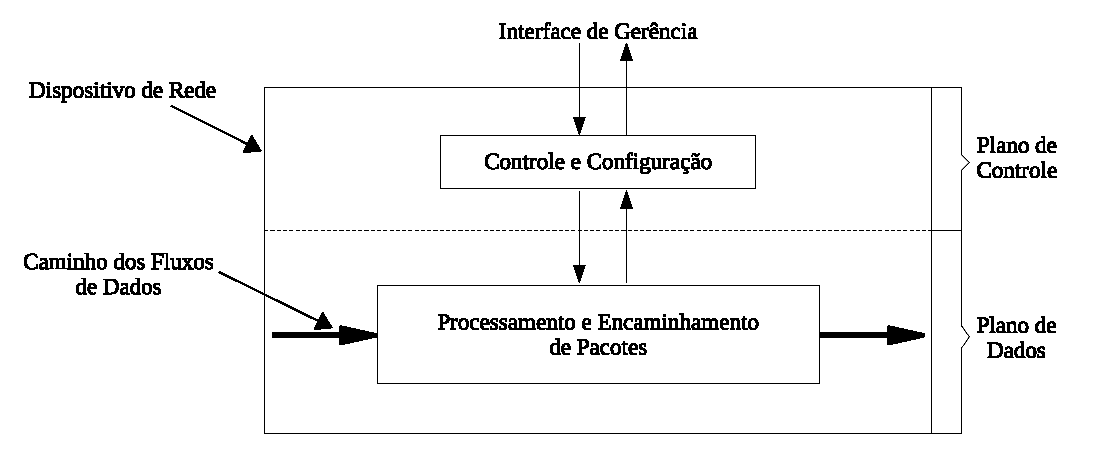
\includegraphics[width=.9\textwidth]{images/planos-introducao.eps}
  \fonte{Comer, 2013. \nocite{Comer:2013}}
  \label{fig:planos-introducao}
  
\end{figure}
\FloatBarrier

Para tentar contornar esse problema, a comunidade de pesquisa em redes de computadores tem investido em iniciativas que levem a implantação de redes com maiores recursos de programação, de forma que novas tecnologias possam ser inseridas na rede de forma gradual. Exemplos de iniciativas desse tipo são as propostas de redes ativas (\textit{active networks}) \cite{Tennenhouse:1997}, de \textit{testbeds} como o PlanetLab \cite{Chun:2003}, GENI \cite{Turner:2006} e, mais recentemente o FIBRE \cite{Salmito:2014}. Redes ativas, tiveram pouca aceitação pela necessidade de alteração dos elementos de rede para permitir que se tornassem programáveis. Iniciativas mais recentes como PlanetLab, GENI e FIBRE, apostam na adoção de recursos de virtualização para facilitar a transição para novas tecnologias. Apesar de serem consideradas de grande potencial a longo prazo, tais iniciativas ainda enfrentam desafios como garantir o desempenho exigido pelas aplicações utilizadas hoje utilizando-se tais elementos virtualizados \cite{Guedes:2006}.

Uma outra forma de abordar esse problema, consiste em estender o \textit{hardware} de encaminhamento de pacotes de forma mais restrita. Considerando-se que a operação que necessita de alto desempenho nos elementos de comutação é o encaminhamento de pacotes (plano de dados), algumas iniciativas propõem manter essa operação pouco alterada, para manter a viabilidade de desenvolvimento de hardware de alto desempenho, mas com uma possibilidade de maior controle por parte do administrador da rede. 

\gls{sdn} introduz uma perspectiva flexível para programar e manter a operacionalidade da rede  buscando desacoplar os planos de dados e de controle, desta forma, tira-se a autonomia dos equipamentos de rede que se tornam apenas encaminhadores de pacotes. Já a lógica de controle é movida para uma entidade externa, centralizada, implementada em \textit{software}. Esta, chamada de controlador, tem por funcionalidade prover a lógica de funcionamento da rede o que torna o desenvolvimento de serviços mais facilmente implementáveis, já que não há a necessidade de implementação em cada dispositivo. 

No plano de dados, o encaminhamento de pacotes, que antes era baseado em destino, passa a ser por fluxo que é definido pela combinação de campos das camadas de enlace, de rede ou de transporte, segundo o modelo TCP/IP. Dessa forma mantém-se o alto desempenho no encaminhamento de pacotes em \textit{hardware}, aliado à flexibilidade de se implementar aplicações em \textit{software}, utilizando protocolo aberto para programação da lógica do equipamento que é abstraída dos dispositivos de encaminhamento \cite{Kim:2013, Tootoonchian:2010, Rothenberg:2010}.

Pensando nisso, nasceu o OpenFlow \cite{McKeown:2008}, que por sua vez, deu origem ao conceito de \textit{Software Defined Networking}, ou redes definidas por software. A Figura \ref{fig:arch-old-sdn} apresenta um comparativo entre o modelo tradicional de rede, onde ambos os planos, de controle e de dados, são localizados em um mesmo dispositivo e o modelo \gls{sdn} que possui controle centralizado e apenas o plano de dados no dispositivo comutador.

\begin{figure}[H]
  \centering
  \caption{Modelos de rede tradicional e SDN}
  \includegraphics[width=.80\textwidth]{images/arch-old-sdn.eps}
  \fonte{Rothenberg \textit{et al.}, 2010. \nocite{Rothenberg:2010}}
  \label{fig:arch-old-sdn}
\end{figure}
\FloatBarrier

O protocolo OpenFlow é implementado em ambos os planos e dispõe de um protocolo de comunicação entre o controlador e \textit{switches}. Para garantir a confiabilidade dessa comunicação é recomendada a utilização do protocolo \gls{ssl} \cite{RFC6101} porém algumas alternativas incluem \gls{tcp}, utilizadas especialmente em redes virtuais devido à sua simplicidade, pois não necessitam de chaves criptográficas \cite{Rothenberg:2010}.

OpenFlow explora a existência de tabelas de fluxo (\textit{flow tables}) em dispositivos \textit{Ethernet} modernos. Essas tabelas são alimentadas em tempo de execução e utilizadas para implementar \textit{firewalls} \cite{Oppliger:1997}, \gls{nat} \cite{RFC3022}, \gls{qos} \cite{Aurrecoechea:1998} e coleta de estatísticas. Normalmente são proprietárias mas há um conjunto de funções que são comuns na maioria dos dispositivos. Com isso, uma forma padrão de manipulação das tabelas de fluxo pode ser implementada, independente de fornecedor. Desta maneira, OpenFlow fornece um padrão para manipulação das tabelas de fluxo, permitindo assim a partição do tráfego, o agrupamento ou isolamento da rede e o processamento ou controle do fluxo de dados, da forma desejada com base no fluxo \cite{Kontesidou:2009}.

Os principais componentes de uma arquitetura \gls{sdn} são:
\begin{itemize}
    \item Comutadores (\textit{switches}) \textit{OpenFlow};
    \item Controlador; e
    \item Protocolo de comunicação.
\end{itemize}
Estes componentes podem fazer uso do protocolo OpenFlow e/ou de outros protocolos. Por ser o primeiro e também o mais utilizado, o protocolo OpenFlow é utilizado neste trabalho como padrão de comunicação entre os dispositivos.

%=====================================================================

\subsection{Comutadores}
\label{subsec:comutador}

É o elemento responsável pelo encaminhamento dos pacotes pela rede. Pode ser específico para OpenFlow, ou ter suporte ao mesmo. No comutador (\textit{switch}) OpenFlow é mantida uma tabela de fluxo (\textit{flow table}) que armazena informações sobre como os pacotes serão processados, estatísticas, prioridades e tempo limite para novos fluxos. Além disso, cada regra é composta por um conjunto de campos do cabeçalho do pacote que podem ser visualizadas na Figura \ref{fig:flow-table}, assim como as informações de ações e estatísticas.

\begin{figure}[H]
  \centering
  \caption{Tabela de fluxo}
  \includegraphics[width=.65\textwidth]{images/flow-table.eps}
  \label{fig:flow-table}
  \fonte{Adaptado de Costa, 2014 \nocite{Costa:2004}}
\end{figure}
\FloatBarrier
%Copiado e artigo 6, reescrever
Quando um pacote chega a um equipamento com OpenFlow habilitado, os cabeçalhos do pacote são comparados (\textit{match}) às regras das entradas das tabelas de fluxos, os contadores são atualizados e as ações correspondentes são realizadas. Se não houver correspondência  (\textit{table miss}) entre o pacote e alguma entrada da tabela de fluxos, o pacote é encaminhado, por completo, ao controlador. Alternativamente, apenas o cabeçalho é encaminhado ao controlador mantendo o pacote armazenado no \textit{buffer} do \textit{hardware}. A Figura \ref{fig:fluxo-tmp} ilustra, através de um diagrama simplificado, o tratamento recebido por pacotes em um \textit{switch} OpenFlow.

Os pacotes que chegam ao controlador normalmente correspondem ao primeiro pacote de um novo fluxo ou, em função do tipo de pacote e da aplicação, o controlador pode decidir por instalar uma regra no \textit{switch} para que todos os pacotes de determinado fluxo sejam enviados para o controlador para serem tratados individualmente. Esse último caso corresponde, em geral, a pacotes de controle  (\gls{icmp} \cite{RFC0792}, \gls{dns} \cite{RFC7719}, \gls{dhcp} \cite{RFC2131}) ou de protocolos de roteamento  (\gls{ospf} \cite{RFC2328}, \gls{bgp} \cite{RFC4271}).
Todos os pacotes de uma mesma faixa de endereços \gls{ip}, ou uma conexão \gls{tcp} em determinada porta são considerados fluxos.

\begin{figure}[H]
  \centering
  \caption{Diagrama simplificado do tratamento de um pacote no \textit{switch} OpenFlow}
  \includegraphics[width=.80\textwidth]{images/flow.eps}
  \label{fig:fluxo-tmp}
  \fonte{Elaborado pelo autor a partir da especificação OpenFlow\\\cite{OpenFlowSpec:2014}}
\end{figure}
\FloatBarrier

A cada pacote recebido, é realizada a atualização dos contadores na tabela de fluxo.
Esses contadores são usados para geração de estatísticas, de maneira a monitorar o número de pacotes e bytes de cada fluxo, além do tempo de duração desde o seu início. O Quadro \ref{tab:contadores} apresenta alguns dos contadores disponíveis na tabela de fluxo. Com o auxílio deste podem ser implementados recursos de monitoramento e segurança do tráfego na rede.

\begin{table}[H]
  \centering
  %\captionof{figure}[tab:contadores]{Contadores da tabela de fluxo}
  \caption{Contadores da tabela de encaminhamento}
  \begin{tabular}{|l|c|} \hline
	\textbf{Contator} & \textbf{Tamanho em bits} \\ \hline
	\multicolumn{2}{|c|}{Por Tabela} \\ \hline
	Número de entradas Ativas & 32 \\ \hline
	Número de pacotes pesquisados & 64 \\ \hline
	Número de pacotes encontrados na tabela & 64 \\ \hline
	\multicolumn{2}{|c|}{Por fluxo} \\ \hline
	Número de pacotes recebidos & 64 \\ \hline
	Número de bytes recebidos & 64 \\ \hline
	Duração (segundos) & 32 \\ \hline
	Duração (nano segundos) & 32 \\ \hline
	\multicolumn{2}{|c|}{Por porta} \\ \hline
	Número de pacotes recebidos & 64 \\ \hline
	Número de pacotes transmitidos & 64 \\ \hline
	Número de bytes recebidos & 64 \\ \hline
	Número de bytes transmitidos & 64 \\ \hline
	Número de pacotes perdidos no recebimento & 64 \\ \hline
	Número de pacotes perdidos na transmissão & 64 \\ \hline
	Número de erros recebidos & 64 \\ \hline
  \end{tabular}
  \label{tab:contadores}
  \fonte{Elaborado pelo autor a partir da especificação OpenFlow\\  \cite{OpenFlowSpec:2014}}
\end{table}

Neste projeto o comutador a ser utilizado é o Open vSwitch \cite{website:ovs}, um \textit{switch} virtual com suporte a OpenFlow. Este comutador é projetado para permitir a automatização de grandes redes através da extensão programática, suportando ainda interfaces e protocolos de gerenciamento como, por exemplo, NetFlow \cite{rfc3954}, sFlow \cite{rfc3176} e IPFIX \cite{rfc5153}. Além disso, pode suportar a distribuição através de múltiplos servidores físicos \cite{website:ovs}.
%=====================================================================

\subsection{Controlador}
\label{subsec:controlador}

O controlador, como já citado, é o \textit{software} responsável por tomar decisões e adicionar e remover as entradas na tabela de encaminhamento, de acordo com o objetivo desejado. Exerce a função de uma camada de abstração da infraestrutura física, facilitando a criação de aplicações e serviços que gerenciem as entradas de fluxos na rede. Esse modelo assemelha-se a outros sistemas de \textit{software} que proveem abstração do \textit{hardware} e funcionalidade reutilizável. Dessa forma, o controlador atua como um \gls{so} para gerenciamento e controle das redes, e oferece uma plataforma com base na reutilização de componentes e na definição de níveis de abstração. Contudo, novas aplicações de rede podem ser desenvolvidas rapidamente \cite{Gude:2008}.

O controlador fornece uma interface para criar, modificar e controlar o fluxo de tabelas do comutador. É executado normalmente em um servidor conectado à rede e pode ser um para todos os comutadores da rede, um para cada comutador ou um para um conjunto de comutadores.  Portanto, a funcionalidade da rede de controle pode ser completamente ou localmente centralizada dependendo de como o gerenciamento dos comutadores é realizada. A exigência, no entanto, é que, se houver mais do que um controlador de processos, eles devem ter a mesma visão da topologia da rede, em qualquer momento dado. A visão de rede inclui a topologia a nível de \textit{switch}, as localizações dos usuários, \textit{hosts}, \textit{middleboxes} e outros elementos de rede e serviços. Além disso inclui todas as ligações entre os nomes e endereços.

O controlador é parte integrante de uma arquitetura de rede \gls{sdn} e para que sua comunicação com \textit{switches} OpenFlow ocorra, o controlador deve ter suporte ao mesmo. Atualmente, existem várias implementações controlador disponíveis que implementam o protocolo OpenFlow, entre os principais não comerciais estão \cite{Kreutz:2013,Xia:2015}:

\begin{itemize}
    \item \textbf{NOX} - Desenvolvido em C++, foi o primeiro controlador OpenFlow \cite{Gude:2008}. Porém não foi fortemente utilizado por causa de deficiências na sua implementação e na documentação.
    \item \textbf{POX} - Sucessor do NOX, foi desenvolvido como uma alternativa mais amigável e tem sido implementado por um grande número de engenheiros e programadores \gls{sdn}. Comparando com NOX, POX tem um ambiente de desenvolvimento mais fácil de trabalhar com uma API razoavelmente bem escrita e documentada. Também fornece uma interface Web e é escrito em Python \cite{website:pox}.
    \item \textbf{Beacon} - É um controlador SDN bem escrito e organizado. Escrito em Java, Beacon foi o primeiro controlador com o qual iniciantes pudessem trabalhar e criar um ambiente \gls{sdn}, no entanto, era limitado à topologias de rede estrela \cite{Erickson:2013}.
    \item \textbf{Floodlight} - Uma ramificação do Beacon. Enquanto que seu início tenha sido baseado no Beacon este foi desenvolvido utilizando Apache Ant, uma ferramenta popular para compilação e construção de \textit{software}, o que tornou o desenvolvimento do Floodlight mais fácil e flexível. Floodlight possui uma comunidade ativa e um grande número de recursos que podem ser adicionados ao sistema. Possui interface baseada em java e baseada em Web, além de possuir uma Interface de Programação de Aplicações (\gls{api}) \gls{rest} ou, em português, Transferência de Estado Representacional \cite{website:floodlight}.
    \item \textbf{OpenDayLight} - É um projeto colaborativo da Linux Fundation e tem sido altamente suportado por empresas como Cisco e Big Switch. Desenvolvido em Java, também inclui \gls{api} \gls{rest} e interface web. Possui suporte à \gls{sdn}, \gls{nv} , ou Virtualização de redes \cite{Chowdhury:2009} e \gls{nfv}, ou Virtualização da Funções da Rede \cite{Hawilo:2014}. Além disso, possui um grande número de módulos que podem ser utilizados para atender aos requisitos de uma organização \cite{website:odl}.
    \item \textbf{Ryu NOS} - É um \textit{framework} de \gls{sdn} baseado em componentes. O Ryu fornece componentes de software com \glspl{api} bem definidas que tornam mais fácil para os desenvolvedores criar novas aplicações de gerenciamento e controle de rede. O Ryu suporta vários protocolos para gerenciar dispositivos de rede, como OpenFlow, Netconf, OF-config, etc. Sobre o OpenFlow, o Ryu suporta totalmente as extensões 1.0, 1.2, 1.3, 1.4, 1.5 e Nicira. Todo o código está disponível gratuitamente sob a licença Apache 2.0 \cite{website:ryu}.
\end{itemize}

%=====================================================================

\subsection{Protocolo OpenFlow}
\label{subsec:protocolo-comunicacao}

O protocolo de comunicação entre os dois planos é realizado por três tipos de mensagens: controlador para o \textit{switch}, assíncrona e simétricas. 

Mensagens do tipo controlador para \textit{switch} são mensagens que o controlador envia para obter informações sobre o estado do \textit{switch}, como por exemplo verificar estatísticas de um determinado fluxo \cite{OpenFlowSpec:2014}. Essas mensagens podem ser:
%Rescrever
\begin{itemize}
    \item \textit{\textbf{Features}}: ao estabelecer uma conexão, o controlador envia esta mensagem requisitando que o \textit{switch} informe suas capacidades.
    \item \textit{\textbf{Configuration}}: o controlador envia parâmetros de configuração para os \textit{switches}. 
    \item \textit{\textbf{Modify-State}}: utilizado pelo controlador para gerenciar o estado dos \textit{switches}, deletar ou modificar regras na tabela de fluxos.
    \item \textit{\textbf{Read-State}}: utilizado pelo controlador para coletar estatísticas das tabelas de fluxos do \textit{switch}.
    \item \textit{\textbf{Packet-Out}}: utilizada pelo controlador para enviar pacotes por uma porta específica.
    \item \textit{\textbf{Barrier}}: utilizada para verificar se as dependências das mensagens foram alcançadas ou receber notificação sobre tarefas concluídas.
     \item \textit{\textbf{Role Request}}: mensagens usadas pelo controlador para configurar seu canal OpenFlow.
\end{itemize}

Mensagens assíncronas são enviadas pelo \textit{switch} sem a solicitação do controlador. \textit{Switches} enviam mensagens assíncronas para os controladores para denotar uma chegada de pacotes ou mudança de estado \cite{OpenFlowSpec:2014}. Os principais tipos de mensagens assíncronas são descritas abaixo.
\begin{itemize}
    \item \textit{\textbf{Packet-In}}: enviado pelo \textit{switch} quando há uma ação explícita na tabela de fluxos para que seja enviado para o controlador ou quando não há um \textit{match} para o pacote.
    \item \textit{\textbf{Flow-Removed}}: informa o controlador sobre a remoção de regras no \textit{switch}.
    \item \textit{\textbf{Port Status}}: informa o controlador sobre uma mudança em alguma porta.
    \item \textit{\textbf{Role Status}}: \textit{switch} informa o controlador sobre a alterações em suas regras.
    \item \textit{\textbf{Controller Status}}: \textit{switch} informa o controlador sobre a mudança em um canal OpenFlow.
    \item \textit{\textbf{Flow-monitor}}: informa o controlador sobre uma mudança na tabela de fluxo.
\end{itemize}

Finalmente, mensagens simétricas são iniciadas tanto pelo controlador como pelo \textit{switch} sem nenhuma solicitação, por exemplo o início de conexão entre controlador e \textit{switch} \cite{OpenFlowSpec:2014}. Essas mensagens são:
\begin{itemize}
    \item \textit{\textbf{Hello}}: esta mensagem é utilizada no início da conexão entre \textit{switch} e controlador.
    \item \textit{\textbf{Echo}}: utilizado para obter informações sobre a conexão entre \textit{switch} e controlador como:
latência, largura de banda e conectividade.
    \item \textit{\textbf{Error}}:  o \textit{switch} pode enviar mensagens para notificar problemas ao controlador por mensagens de erro.
    \item \textit{\textbf{Experimenter}}: na versão 1.5.0 do protocolo OpenFlow, esta mensagem é utilizada para adicionar funcionalidades experimentais.
\end{itemize}

Cada mensagem é enviada encapsulada em um pacote definido pelo protocolo OpenFlow e que é representado na Figura \ref{fig:openflow-message}.

\begin{figure}[H]
  \centering
  \caption{Formato da mensagem OpenFlow}
  \includegraphics[width=.80\textwidth]{images/openflow-message.eps}
  \label{fig:openflow-message}
  \fonte{\centering
  Elaborado pelo autor a partir de informações da especificação OpenFlow.}
\end{figure}
\FloatBarrier

O campo \textit{version} indica a versão do protocolo que está sendo utilizada. Já o  \textit{type}, indica o tipo de mensagem que está sendo enviada. O campo \textit{length} informa o tamanho da mensagem enquanto que \textit{xid} representa o ID de transação associado à mensagem. Por último, o campo \textit{payload} representa o corpo da mensagem, é neste campo onde são adicionados os diferentes tipos de mensagens apresentados anteriormente.
\section{Virtualização}
\label{sec:virtualizacao}
%Rescrever

O conceito de virtualização de redes define uma infraestrutura de redes de computadores virtuais. São definidos por \textit{software}, executando sobre máquinas físicas, de forma que toda infraestrutura virtual seja isolada da infraestrutura física, não interferindo na mesma. 

Um dos \textit{softwares} mais usados na criação de redes virtuais em nível de \textit{software} é o Xen \cite{Fernandes:2011}. Esse programa é usado na criação de máquinas virtuais em computadores pessoais e servidores, e oferece a opção de criar roteadores virtuais que podem ser utilizados na interligação de máquinas virtuais para a formação de uma rede. Em \gls{sdn} a construção de redes virtuais acontece em nível de \textit{hardware}, através da separação do tráfego da rede física em \textit{slices}, porções de fluxo do tráfego total. O FlowVisor \cite{Sherwood:2009} possibilita virtualização em \gls{sdn}.

O uso de virtualização de redes possibilita execução de experimentos distintos, sobre a mesma infraestrutura, em paralelo, sem interferência entre experimentos. Virtualização de redes também pode ser usada para isolamento de serviços. Assim, uma organização pode oferecer diversos serviços, com cada serviços executando em uma rede virtual diferente \cite{wu:2010, Mattos:2012}.

\section{Emulador Mininet}
\label{sec:mininet}

Mininet \cite{Handigol:2012} é um emulador de rede para prototipação em \gls{sdn}. A razão pela sua utilização deve-se ao fato de apenas alguns dispositivos de rede estarem disponíveis para \gls{sdn}, uma vez que ainda não é uma tecnologia difundida a nível industrial.  Além disso, a implementação de rede com elevado número de dispositivos de rede é muito difícil e dispendioso. Por isso, para contornar estes problemas, a virtualização foi realizada com a finalidade de prototipar e emular este tipo de tecnologia de rede e um dos mais importantes é o Mininet \cite{Wendong:2012}.  Mininet tem a capacidade de emular diferentes tipos de elementos de rede, tais como: \textit{host}, \textit{switches} (camada de enlace), roteadores (camada de rede) e conexões. Ele funciona em um único núcleo de Linux\cite{Negus:2015} e utiliza virtualização com a finalidade de emular uma rede completa que utiliza apenas um único sistema. No entanto, o \textit{host}, roteadores e links criados são elementos do mundo real, embora eles sejam criados por meio de software \cite{website:mininet}.

Criar uma rede no Mininet é relativamente simples. Pode-se usar linha de comando ou um componente chamado \textit{miniedit.py}, que implementa uma interface gráfica para o Mininet, este porém, possui algumas limitações em relação à linha de comando. Pela linha de comando, ao chamar o Mininet são passados os parâmetros sobre as características da rede como: topologia, número de \textit{hosts}, \textit{switches}, taxa de perda de pacotes, largura de banda, tipo de controlador, entre outros. O \textit{switch} padrão é o OpenSwitch \cite{Pettit:2010}, um \textit{switch} virtual desenvolvido especialmente para trabalhar com o protocolo Openflow. Para estudo mais aprofundado, recomenda-se a leitura da sua documentação em \cite{website:mininet}.
\section{Segurança em redes}
\label{sec:seguranca}

A segurança no nível de rede indica uma área de pesquisa muito importante, já que os usuários estão continuamente colocando seus dados em ambientes em nuvem e mais dados são transferidos através de grandes distâncias. A razão para esta evolução é a crescente popularidade dos serviços em nuvem, bem como a simplicidade e rápida capacidade dos recursos sob demanda. Os impactos variam de acordo com os tipos de ameaças, e como defesa são criados diversos sistemas de segurança que agem como barreira de proteção, como por exemplo, \textit{firewalls}. Os principais tipos de ameaças serão estudadas a seguir. Também é apresentado um estudo mais detalhado do ataque do tipo varredura, foco deste trabalho.

\subsection{Tipos de ameaças}
Dos diversos tipos de ameaças que podem ocorrer nas redes de computadores, destacam-se algumas que são notórias por causar frequentes transtornos aos usuário, tais como:

\textbf{Fraude}:
Segundo Houaiss, Villar e Francisco (2001)\nocite{Houaiss:2001}, é "qualquer ato ardiloso, enganoso, de má-fé, com intuito de lesar ou ludibriar outrem, ou de não cumprir determinado dever; logro". Esta categoria engloba as notificações de tentativas de fraudes, ou seja, de incidentes em que ocorre uma tentativa de obter vantagem, sejam por meios como correios eletrônicos não solicitados em massa (\textit{spam}) e páginas falsas.
    
\textbf{Ataque de negação de serviço (\textit{\gls{dos}}}:
Um ataque de negação de serviço busca sobrecarregar serviços na rede dificultando o seu uso por usuários legítimos. Esse tipo de ataque, por sua natureza, pode produzir variações no volume de tráfego que normalmente são visíveis no gráfico de fluxo. Segundo Sperotto \textit{et al.} (2010)\nocite{Sperotto:2010} no entanto, na detecção de intrusão por fluxo, é abordado implicitamente o problema de ataques \gls{dos} por força bruta, ou seja, um tipo de \gls{dos} que depende de esgotamento de recursos ou sobrecarga da rede. Infelizmente, é quase impossível de detectar diretamente ataques \gls{dos} semânticas.
    
\textbf{Infestações viróticas automatizadas (\textit{Worms})}:
São pequenos programas de computador criados para causar danos na máquina infectada e se auto replica pela rede, tirando cópias de si em cada computador \cite{Sperotto:2010}.
    
\textbf{Exército de máquinas controladas sem autorização (\textit{Botnets})}:
Grupo de computadores comprometidos, chamados de computadores zumbis que são controlados remotamente por um centro de controle. \textit{Botnets} são muito utilizados para lançamento de ataques  como \textit{spams}, DoS e \textit{worms} \cite{Sperotto:2010}.
    
\textbf{Varredura de portas maliciosa (\textit{port scans})}:
Técnica utilizada para encontrar fraquezas de um computador ou de uma rede. Enquanto esta técnica não é um ataque real, os hackers a usam para detectar quais portas estão abertas em um computador. Baseado nas informações sobre portas abertas, o acesso não autorizado pode ser obtido.

Os métodos citados também podem também ser utilizados em conjunto, como por exemplo a utilização de \textit{botnets} que, controlados remotamente, podem efetuar ataques DoS a um mesmo servidor e ao mesmo tempo. A esse tipo de ataque é dado o nome de Negação de Serviço Distribuída (\gls{ddos})

Do ponto de vista de segurança, existe uma quantidade crescente de incidência de ataques de negação de serviço, \gls{dos}, durante os últimos anos \cite{Seeber:2015}. Além disso, segundo a \gls{cert.br}, responsável por tratar incidentes de segurança e computadores que envolvam redes conectadas à Internet brasileira, foram reportados 722.205 incidências de segurança somente no ano de 2015, sendo mais da metade (53\%), ataques do tipo \textit{port scan}.

\subsection{Técnicas de varredura}
\label{sec:varredura}

Um dos tipos mais comuns de ataques, a varredura consiste no envio de diversos tipos de pacotes com o intuito de se conhecer mais sobre o nó alvo ou a rede em questão. Através das respostas obtidas para esses pacotes, o atacante é capaz de chegar a diversas informações que possam ajudar em futuros ataques de diversos tipos. Alguns tipos de informações que podem ser descobertas incluem (não somente): A atividade dos servidores, informações relativas a softwares utilizados no sistema, informações sobre o \textit{firewall} e topologia da rede.

Uma das principais dificuldades nas soluções desse tipo de ataque é que as varreduras são consideradas atividades legais, e ocorrem na Internet de forma rotineira, inclusive com fins não maliciosos.

Antes de explorar as técnicas de varredura, faz-se necessário o entendimento de alguns conceitos de comunicação \gls{tcp}. Para obter um serviço \gls{tcp}, uma conexão necessita ser efetivada entre os computadores origem e destino. Esta conexão é realizada através dos chamados \textit{sockets}, formados pelo par endereço \gls{ip} e número de porta, de ambos, computador de origem e computador de destino. Entre estes dois \textit{sockets} ocorre a transferência de segmentos.

Um segmento consiste em um cabeçalho \gls{tcp} seguido, opcionalmente, por informação. Um cabeçalho \gls{tcp} pode possuir seis \textit{flags} que podem ser ativadas ou desativadas ao mesmo tempo \cite{Comer:2013}, são elas:

\begin{itemize}
    \item \textbf{SYN} - \textit{bit} de sincronismo, é o \textit{bit} que informa que este é um dos dois primeiros segmentos de estabelecimento da conexão.
    \item \textbf{ACK} - \textit{bit} de reconhecimento, indica que o valor do campo de reconhecimento está carregando um reconhecimento válido.
    \item \textbf{PSH} - \textit{bit} de \textit{push}, este mecanismo, que pode ser acionado pela aplicação, informa ao \gls{tcp} origem e destino que a aplicação solicita a transmissão rápida dos dados enviados, mesmo que ela contenha um número baixo de \textit{bytes}, não preenchendo o tamanho mínimo do \textit{buffer} de transmissão.
    \item \textbf{RST} - \textit{bit} de \textit{reset}, informa o destino que a conexão foi abortada neste sentido pela origem
    \item \textbf{FIN} - \textit{bit} de terminação, indica que este pacote é um dos pacotes de finalização da conexão.
\end{itemize}

Em uma comunicação \gls{tcp}, uma conexão deve ser estabelecida entre os dois pontos (\textit{sockets}) para que a transferência de dados ocorra.
Inicialmente a máquina emissora, também chamada de cliente, transmite um segmento cuja \textit{flag} SYN é de 1 (para assinalar que se trata de um segmento de sincronização), com um número de ordem X, que se chama número de ordem inicial do cliente.

A seguir, a máquina receptora, chamada de servidor, recebe o segmento inicial que provém do cliente e envia-lhe um aviso de recepção, isto é, um segmento cuja \textit{flag} ACK é de 1 e a \textit{flag} SYN é de 1 (porque ainda se trata de uma sincronização). Este segmento contém o número de ordem do servidor, que é o número de ordem inicial do cliente. O campo mais importante deste segmento é o campo de aviso de recepção, que contém o número de ordem inicial do cliente, incrementado de 1.

Por último, o cliente transmite ao servidor um aviso de recepção, ou seja, um segmento cuja \textit{flag} ACK é de 1, cuja \textit{flag} SYN é de zero (não se trata mais de um segmento de sincronização). O seu número de ordem é incrementado e o número de aviso de recepção representa o número de ordem inicial do servidor, incrementado de 1.

Depois dessa sequência de trocas (Figura \ref{fig:troca-tcp}), também chamada de \textit{handshake}, ou, aperto de mãos em português, as duas máquinas estão conectadas e a comunicação pode ser efetivada.

\begin{figure}[H]
  \centering
  \caption{Estabelecimento de conexão TCP}
  \includegraphics[width=0.5\textwidth]{images/conexao-tcp.eps}
  \label{fig:troca-tcp}
   \fonte{Elaborado pelo autor.}
\end{figure}
\FloatBarrier

Os passos a seguir são definidos pela RFC 793 \cite{rfc793}, utilizada pela grande maioria das implementações \gls{tcp} e exploradas em técnicas de varredura.

\begin{itemize}
    \item Quando um segmento SYN chega em um aporta aberta, é continuado o procedimento de \textit{handshake} como discutido anteriormente; 
    \item Quando um segmento SYN (ou FIN) chega em uma porta fechada, o segmento é descartado e um segmento RST é retornado para o cliente;
    \item Quanto um segmento FIN chega em uma porta que esteja aberta, o segmento é descartado.
    \item Quando um segmento RST chega em uma porta que esteja ouvindo (aberta), o segmento é descartado;
    \item Quando um segmento RST chega em uma porta que não esteja ouvindo (fechada), o segmento é descartado;
    \item Quando um segmento ACK chega à uma porta aberta, o mesmo é descartado e retornado um segmento RST.
\end{itemize}


Devido à sua natureza, \textit{scans} podem facilmente criar um vasto número diferente de fluxos. Segundo Speroto \textit{et al.} (2010)\nocite{Sperotto:2010}, há três categorias de varredura, são elas:
\begin{itemize}
    \item \textbf{\textit{scan} horizontal} - quando um \textit{host} de origem varre uma porta especifica em diferentes \textit{hosts} alvo;
    \item \textbf{\textit{scan} vertical} - quando um \textit{host} de origem verifica várias portas distintas de um mesmo \textit{host} alvo; e
    \item \textbf{\textit{scan} misto} - quando há a combinação das varreduras vertical e horizontal.
\end{itemize}

Existem várias técnicas de varredura de porta disponíveis e podem facilmente ser automatizadas por ferramentas como Nmap \cite{Lyon:2009}. Alguns métodos utilizados para varredura são estudados a seguir \cite{deVivo:1999, Christopher:2001}.
\begin{itemize}
\item \textbf{\textit{TCP Connect}} - É a forma mais comum de \textit{scanning}. Basicamente uma conexão TCP regular (\textit{handshake} completo) para cada porta definida na varredura. Para cada porta, a conexão pode resultar em sucesso, indicando uma porta aberta ou em falha caso contrário. Essa técnica é facilmente implementada pois não necessita de privilégios especiais e, do mesmo modo, é facilmente detectável. Através de \textit{logs} do sistema alvo é possível verificar mensagens de requisição de conexão e de erro para as conexões negadas. Neste método, o \textit{scanner} envia uma mensagem SYN para o sistema alvo. Se uma porta estiver (aberta) ouvindo com um serviço, a conexão se sucederá. Um SYN é retornado estabelecendo o número de sequência inicial. Um ACK considera o campo numérico de confirmação válido. Se a porta estiver (fechada) sem serviço ouvindo, uma mensagem RST é retornada, para reiniciar o pedido de conexão. Alguns exemplos de \textit{scanners} podem ser Nmap, Amap e Blaster. %Exemplo de \textit{scanner}: nmap.

\item \textbf{TCP SYN} - Também conhecida por \textit{Half Open} por não explorar um \textit{handshake} completo. Nesta técnica o \textit{scanner} envia uma mensagem SYN, como se estivesse pedindo uma conexão. Se responder como um RST, indica que a porta está fechada, e uma nova porta é testada. Se a resposta da máquina alvo for um SYN/ACK, indica que a porta se encontra ouvindo. O \textit{scanner} envia então um RST cancelando o \textit{handshake}. A vantagem desse tipo de \textit{scanning} é o fato de, mesmo ainda podendo ser detectado, tentativas de conexões SYN são menos frequentemente registradas se comparadas com conexões \gls{tcp} completas. %Exemplos de \textit{scanners}: amap, hping2, netstat, nmap.

\item \textbf{Exploração FIN} - Neste método, quando um segmento FIN é enviado para uma porta fechada, o computador alvo responde com um TCP RST. Quando a porta estiver aberta, o segmento é ignorado e o computador alvo não responde. O \textit{scanner} não recebe nunhuma resposta, pois não podem pertencer a uma conexão estabelecida. %Exemplos de \textit{scanners}: hping2, nmap.

\item \textbf{Xmas Tree} - é uma variação do método TCP FIN, neste, são utilizadas mensagens com prioridade TCP FIN/URG/PSH. Quando estiver ouvindo, o \textit{host} alvo não responde, caso contrário, responde com um TCP RST. %Exemplos de \textit{scanners}: hping2, netstat, nmap.

\item \textbf{TCP Null (sem flags ativos)} - também é uma variação do método TCP FIN, neste, tem-se resposta para portas fechadas, mas não para portas abertas.% Exemplos de \textit{scanners}: hping2, netstat, nmap.

\item \textbf{Varredura ACK} - Técnica utilizada para identificar \textit{firewalls}. Um segmento ACK que não pertença a nenhum conexão é gerado pelo \textit{scanner}. Se um RST é devolvido pela máquina alvo, tanto em uma porta aberta como em uma fechada, as portas são classificadas como não tendo \textit{firewall}.

\item \textbf{Varredura ARP} - Não se trata exatamente de varredura de portas mas essa técnica é utilizada para descobrir dispositivos ativos na rede local, para depois realizar a varredura de portas somente nos computadores ativos. O \textit{scanner} envia uma série de pacotes de protocolo \gls{arp} \cite{RFC0826} e incrementa o valor do \gls{ip} alvo a cada \textit{broadcast}.
\end{itemize}


\subsection{Ferramentas de Varredura}

Para que as varreduras sejam efetuadas, tem-se a possibilidade de utilizar ferramentas que possibilite a varredura utilizando as diferentes formas citadas na seção anterior. Uma das ferramentas mais utilizadas, e que foi utilizada neste trabalho é o Nmap \cite{Lyon:2009}.

O Nmap é um \textit{software} que oferece uma gama muito grande de recursos e funcionalidades, como detecção do Sistema Operacional remoto, o serviço e a versão que está em uso no host, o exame de ociosidade por identificação (ID) de Internet Protocol (IP), o rápido exame de multiportas por ping entre tantas outras. Possui versões para plataformas Unix, Windows, e MacOS sendo utilizado tanto por interface console como também em interface gráfica, o software Nmap é um utilitário livre e de código aberto, usado para exploração de redes, segurança e auditoria, capaz de examinar grandes redes ou simplesmente um único host.
A função principal do Nmap é realizar uma varredura em portas \gls{tcp} e o retorno dessa varredura é classificado em um dos seguintes estados: aberta, fechada, filtrada, nao filtrada e a combinação de aberta/filtrada ou fechada/filtrada \cite{Lyon:2009}. Vários outros softwares que são utilizados para gerencia e controle de redes de computadores fazem uso do Nmap pois pode ser usado diretamente, sempre que se desejar uma verificação de portas em um \textit{host} que esteja em uma rede local ou na Internet.
O uso mais simples do Nmap é escanear diretamente uma máquina da rede, onde uma quantidade enorme de portas \gls{tcp} será examinada na máquina alvo, e cada porta será classificada de acordo com seu estado.
Na linha de comando do Nmap, tudo que não for uma opção ou argumento de opção será tratado como uma especificação de hospedeiro alvo. O caso mais simples é a especificação de um endereço IP ou nome de hospedeiro alvo para exame \cite{Lyon:2009}.


\subsection{Sistemas de detecção e prevenção de intrusão}

O isolamento da rede em redes virtuais permite uma maior segurança devido ao seu isolamento, porém problemas tradicionais relacionados à segurança continuam existindo em ambientes virtualizados pois 60\% a 70\% dos ataques à segurança da rede são de origem interna segundo Lynch (2006)\nocite{Lynch:2006}. Uma das formas de se proteger desses ataques é monitorar o tráfego em busca de atividades maliciosas ou violação de políticas. Para realizar o monitoramento de pacotes na rede, a solução mais apropriada é o sistema de detecção de intrusão, que realiza o monitoramento passivo dos pacotes na rede. Porém, esse tipo de análise não permite que sejam tomadas ações para prevenir tais ataques, e então faz se necessário um sistema de prevenção de intrusão para bloquear esses pacotes.

Segundo Kruegel (2004)\nocite{Kruegel:2004}, "Detecção de intrusão é o processo de identificar e responder à atividades maliciosas na computação e redes de dados". Uma tentativa de intrusão, também chamada de ataque, refere-se a uma série de ações em que um intruso tenta obter o ganho do sistema e o objetivo de um \gls{ids} é discriminar tentativas de intrusão e preparação de intrusão do uso normal do sistema.

Em redes tradicionais, para detectar e prevenir intrusos maliciosos na rede de dados, administradores normalmente necessitam implantar diversos detectores de intrusão em diferentes locais da rede, e então analisar dados do tráfego coletados localmente ou em um nodo centralizado. Infelizmente, arquiteturas \gls{ids}/\gls{ips} utilizadas atualmente possuem muitas barreiras para gerir nós distribuídos. Em primeiro lugar, os nós de detecção de intrusão devem suportar diferentes configurações. Como as configurações dependem da topologia da rede, configurações manuais e mudanças frequentes são inevitáveis para tornar a política em nós distribuídos eficaz e coerente. Em segundo lugar, algoritmos de detecção de intrusão eficazes normalmente são desenhados para um determinado tipo de ataque. Para desenvolver sistemas de detecção eficazes, mais e mais protocolos de proteção são criados, o que resulta na redução do desempenho da rede. Além disso, dispositivos de rede normalmente possuem protocolos proprietários, o que torna mais difícil desenvolver interfaces de gerenciamento automáticas \cite{Wang:2015}.

Vários trabalhos para \gls{ids} tem sido desenvolvidos desde o início de sua pesquisa nos anos 1980. Essas propostas podem ser classificadas de acordo com várias características, como tipo de dados analisado (\textit{logs} ou dados do pacote), tipo de análise (em tempo real ou \textit{offline}) ou pelo tipo de processamento (centralizado ou distribuído). No entanto, os modelos de classificação mais conhecidos são os baseados em assinatura e os baseados em anomalia \cite{Axelsson:2000}.

Sistemas de detecção de intrusão baseados em assinatura realizam a detecção através da comparação de dados do pacote com uma base de dados conhecida. O \gls{ids} Snort \cite{Roesch:1999} é um dos exemplos mais utilizados dessa técnica, verificando padrões de pacote através da análise de dados da carga útil (\textit{payload}) do pacote. O Snortik \cite{Fagundes16} também é um bom exemplo, neste, é proposto uma integração entre o \gls{ids} Snort e o sistema de \textit{firewall} do sistema MikroTik RouteOS \cite{mikrotik16} com a finalidade de automatizar o processo de reação à ataques. \glspl{ids} baseados em assinatura possuem alta precisão, raramente apresentando alarmes para fluxos normais, porém, não reconhecem fluxos novos, não presentes na sua base de dados. Além disso, a inspeção de pacotes é difícil e até mesmo impossível de ser realizada  em redes com taxas com múltiplos Gigabits por segundo \cite{Lai:2004, Gao:2006}.

Sistemas de detecção de intrusão baseados em anomalia por sua vez, comparam dados recebidos com um "modelo de normalidade" que descreve o comportamento normal da rede. Alterações significativas desse modelo são consideradas como anomalias. Exemplos de criação de comportamentos podem ser redes neurais, técnicas de análise de estatísticas e teoria das probabilidades. A principal vantagem desse tipo de detecção é o fato de também detectar fluxos não conhecidos anteriormente \cite{Owezarski:2010}. No entanto, podem existir casos em que fluxos podem ser diferentes da normalidade esperada mas não necessariamente serem maliciosos resultando em alarmes falsos positivos.

Um \gls{ids} deve ser capaz de lidar com o número crescente do tráfego e ataques na rede. No entanto, alternativas baseadas nas análise de carga útil possuem eficácia em redes entre 100Mbps e 200Mbps \cite{Lai:2004, Gao:2006} podendo chegar a 1Gbps quando hardware dedicado é empregado \cite{Vasiliadis:2008}. Sistemas como Bro \cite{Paxson:1999} e Snort \cite{Roesch:1999} apresentam alto consumo de recursos  quando confrontado com a enorme quantidade de dados de alta taxa de transferência encontrados atualmente \cite{Dreger:2004}. Além disso, protocolos criptografados podem representar um desafio a mais para sistemas de carga útil. Para redes de alta taxas de transmissão, alternativas à inspeção de pacotes são muito importantes. Uma dessas alternativas e que tem atraído pesquisadores é a detecção de intrusão de anomalias baseada em fluxo.

Com esta abordagem, são analisados os padrões de comunicação dentro da rede, ao invés do conteúdo dos pacotes individuais. Hoje em dia os sistemas de medição especiais são capazes de fornecer, para cada par de endereços IP e números de porta, informações agregadas, como a quantidade de bytes transferidos, o número de pacotes enviados e o tempo que determinado fluxo de dados esteve ativo. Essas informações podem então ser exportadas para outros sistemas analisarem, para então, serem usados para detectar intrusões \cite{Sperotto:2010}.

Considerando essa inflexibilidade sobre os equipamentos atuais, os interesses sobre abstrair funções de rede de \textit{switches} dedicados para aplicações \gls{sdn} vem aumentando. Sendo assim, as políticas de segurança podem ser instaladas pelo controlador como regras nas tabelas de fluxo \cite{Kim:2013}, em vez de configurações manuais e independentes. Com isso, o \textit{switch} provê apenas a função de filtro de acordo com a regra na tabela de fluxo, não influenciando significativamente no desempenho da rede. Além disso, \gls{sdn} tem recursos naturais de estatísticas que são úteis para a análise de detecção de intrusão, de modo que o controlador obtém mais visibilidade sobre o tráfego da rede. Portanto, \gls{sdn} parece fornecer uma arquitetura mais adequada para \gls{ips}.



\chapter{Fundamentação Teórica}
\label{cap:fundamentacao}

Neste capítulo serão apresentados tópicos relacionados ao presente trabalho que se fazem necessários para o entendimento deste Trabalho de Conclusão. O capítulo está organizado da seguinte forma: na Seção \ref{sec:sdn-openflow} são abordados os conceitos sobre \gls{sdn} e Openflow; na Seção \ref{sec:virtualizacao} é feita uma abordagem referente a virtualização de redes; na Seção \ref{sec:mininet} é abordado o software de simulação de rede Mininet, utilizado para realização de testes neste trabalho; e por fim, na Seção \ref{sec:seguranca}, é discutido o assunto de segurança em redes de computadores, os principais tipos de ataques e soluções além da ferramenta utilizada para varredura de portas.

\section{Redes Definidas por Software}
\label{sec:sdn-openflow}

As redes de computadores se tornaram parte da infraestrutura crítica de empresas, escolas e residências, tendo crescido bastante desde a sua origem. O sucesso das redes de computadores se deve, em grande parte, à simplicidade de seu núcleo. Na arquitetura atual, a inteligência está localizada nos sistemas de borda, enquanto que o núcleo é simples e transparente. Embora essa simplicidade tenha tido sucesso, também é razão para o seu engessamento, pois apresenta limitações estruturais que são difíceis de serem resolvidas, tais como escalabilidade, mobilidade e gerenciamento de serviço \cite{Clarkl:2004}.

Por causa desta expansão, o trabalho dos pesquisadores da área tornou-se muito mais importante, porém mesmo com o grande número de equipamentos e protocolos criados para suportar essa expansão, ainda tem-se uma grande barreira. A maioria das ideias que surgem não conseguem ser testadas por falta de maneiras práticas que possibilitem a realização de experimentos com novos protocolos em uma rede realista, para que possa obter a confiança necessária para uma implantação em escala global \cite{McKeown:2008}. 

Como apresentado por Kreutz \cite{Kreutz:2014}, redes de computadores podem ser separadas em três planos: de controle, de dados e de gerência. Entende-se por plano de controle a porção da rede que abriga os \textit{softwares} responsáveis por ditar o comportamento da rede. Decisões de roteamento, \textit{firewall}, priorização de pacotes são de responsabilidade do plano de controle. O plano de dados é o que executa o encaminhamento dos pacotes com base nas regras ditadas pelo plano de controle. Já o plano de gerência inclui serviços utilizados para monitorar a rede e configurar remotamente o plano de controle utilizando protocolos como \gls{snmp} \cite{RFC1157}. 

Em síntese, o plano de gerência define as regras da rede, o de controle implementa essas regras e o plano de dados realiza o encaminhamento de pacotes de acordo com as regras impostas pelo plano de controle. Em redes \gls{ip} tradicionais, os planos de controle e dados são acoplados em um mesmo hardware, como pode ser visualizado na Figura \ref{fig:planos-introducao}, tornando a arquitetura de rede complexa e por consequência dificulta a sua configuração e o seu gerenciamento.


\begin{figure}[H]
  \centering
  \caption{Planos de redes de computadores.}
  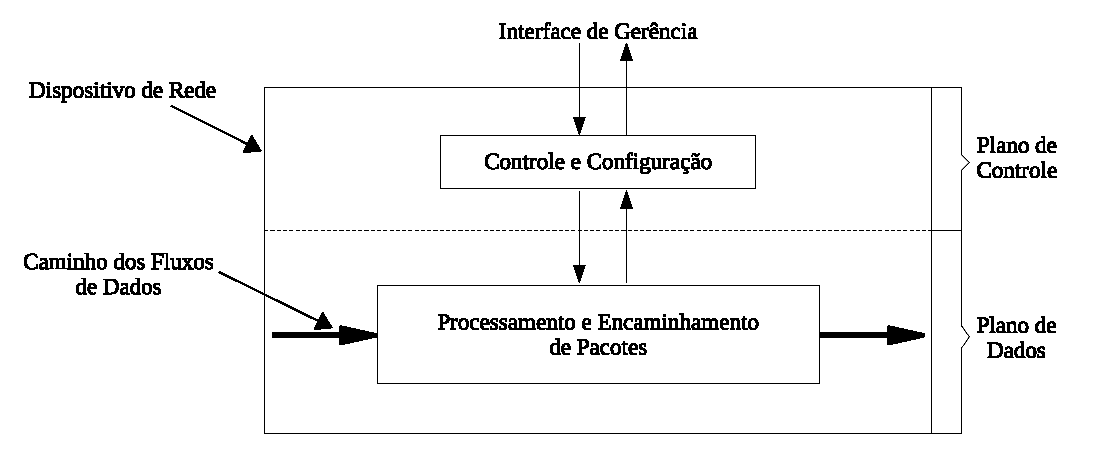
\includegraphics[width=.9\textwidth]{images/planos-introducao.eps}
  \fonte{Comer, 2013. \nocite{Comer:2013}}
  \label{fig:planos-introducao}
  
\end{figure}
\FloatBarrier

Para tentar contornar esse problema, a comunidade de pesquisa em redes de computadores tem investido em iniciativas que levem a implantação de redes com maiores recursos de programação, de forma que novas tecnologias possam ser inseridas na rede de forma gradual. Exemplos de iniciativas desse tipo são as propostas de redes ativas (\textit{active networks}) \cite{Tennenhouse:1997}, de \textit{testbeds} como o PlanetLab \cite{Chun:2003}, GENI \cite{Turner:2006} e, mais recentemente o FIBRE \cite{Salmito:2014}. Redes ativas, tiveram pouca aceitação pela necessidade de alteração dos elementos de rede para permitir que se tornassem programáveis. Iniciativas mais recentes como PlanetLab, GENI e FIBRE, apostam na adoção de recursos de virtualização para facilitar a transição para novas tecnologias. Apesar de serem consideradas de grande potencial a longo prazo, tais iniciativas ainda enfrentam desafios como garantir o desempenho exigido pelas aplicações utilizadas hoje utilizando-se tais elementos virtualizados \cite{Guedes:2006}.

Uma outra forma de abordar esse problema, consiste em estender o \textit{hardware} de encaminhamento de pacotes de forma mais restrita. Considerando-se que a operação que necessita de alto desempenho nos elementos de comutação é o encaminhamento de pacotes (plano de dados), algumas iniciativas propõem manter essa operação pouco alterada, para manter a viabilidade de desenvolvimento de hardware de alto desempenho, mas com uma possibilidade de maior controle por parte do administrador da rede. 

\gls{sdn} introduz uma perspectiva flexível para programar e manter a operacionalidade da rede  buscando desacoplar os planos de dados e de controle, desta forma, tira-se a autonomia dos equipamentos de rede que se tornam apenas encaminhadores de pacotes. Já a lógica de controle é movida para uma entidade externa, centralizada, implementada em \textit{software}. Esta, chamada de controlador, tem por funcionalidade prover a lógica de funcionamento da rede o que torna o desenvolvimento de serviços mais facilmente implementáveis, já que não há a necessidade de implementação em cada dispositivo. 

No plano de dados, o encaminhamento de pacotes, que antes era baseado em destino, passa a ser por fluxo que é definido pela combinação de campos das camadas de enlace, de rede ou de transporte, segundo o modelo TCP/IP. Dessa forma mantém-se o alto desempenho no encaminhamento de pacotes em \textit{hardware}, aliado à flexibilidade de se implementar aplicações em \textit{software}, utilizando protocolo aberto para programação da lógica do equipamento que é abstraída dos dispositivos de encaminhamento \cite{Kim:2013, Tootoonchian:2010, Rothenberg:2010}.

Pensando nisso, nasceu o OpenFlow \cite{McKeown:2008}, que por sua vez, deu origem ao conceito de \textit{Software Defined Networking}, ou redes definidas por software. A Figura \ref{fig:arch-old-sdn} apresenta um comparativo entre o modelo tradicional de rede, onde ambos os planos, de controle e de dados, são localizados em um mesmo dispositivo e o modelo \gls{sdn} que possui controle centralizado e apenas o plano de dados no dispositivo comutador.

\begin{figure}[H]
  \centering
  \caption{Modelos de rede tradicional e SDN}
  \includegraphics[width=.80\textwidth]{images/arch-old-sdn.eps}
  \fonte{Rothenberg \textit{et al.}, 2010. \nocite{Rothenberg:2010}}
  \label{fig:arch-old-sdn}
\end{figure}
\FloatBarrier

O protocolo OpenFlow é implementado em ambos os planos e dispõe de um protocolo de comunicação entre o controlador e \textit{switches}. Para garantir a confiabilidade dessa comunicação é recomendada a utilização do protocolo \gls{ssl} \cite{RFC6101} porém algumas alternativas incluem \gls{tcp}, utilizadas especialmente em redes virtuais devido à sua simplicidade, pois não necessitam de chaves criptográficas \cite{Rothenberg:2010}.

OpenFlow explora a existência de tabelas de fluxo (\textit{flow tables}) em dispositivos \textit{Ethernet} modernos. Essas tabelas são alimentadas em tempo de execução e utilizadas para implementar \textit{firewalls} \cite{Oppliger:1997}, \gls{nat} \cite{RFC3022}, \gls{qos} \cite{Aurrecoechea:1998} e coleta de estatísticas. Normalmente são proprietárias mas há um conjunto de funções que são comuns na maioria dos dispositivos. Com isso, uma forma padrão de manipulação das tabelas de fluxo pode ser implementada, independente de fornecedor. Desta maneira, OpenFlow fornece um padrão para manipulação das tabelas de fluxo, permitindo assim a partição do tráfego, o agrupamento ou isolamento da rede e o processamento ou controle do fluxo de dados, da forma desejada com base no fluxo \cite{Kontesidou:2009}.

Os principais componentes de uma arquitetura \gls{sdn} são:
\begin{itemize}
    \item Comutadores (\textit{switches}) \textit{OpenFlow};
    \item Controlador; e
    \item Protocolo de comunicação.
\end{itemize}
Estes componentes podem fazer uso do protocolo OpenFlow e/ou de outros protocolos. Por ser o primeiro e também o mais utilizado, o protocolo OpenFlow é utilizado neste trabalho como padrão de comunicação entre os dispositivos.

%=====================================================================

\subsection{Comutadores}
\label{subsec:comutador}

É o elemento responsável pelo encaminhamento dos pacotes pela rede. Pode ser específico para OpenFlow, ou ter suporte ao mesmo. No comutador (\textit{switch}) OpenFlow é mantida uma tabela de fluxo (\textit{flow table}) que armazena informações sobre como os pacotes serão processados, estatísticas, prioridades e tempo limite para novos fluxos. Além disso, cada regra é composta por um conjunto de campos do cabeçalho do pacote que podem ser visualizadas na Figura \ref{fig:flow-table}, assim como as informações de ações e estatísticas.

\begin{figure}[H]
  \centering
  \caption{Tabela de fluxo}
  \includegraphics[width=.65\textwidth]{images/flow-table.eps}
  \label{fig:flow-table}
  \fonte{Adaptado de Costa, 2014 \nocite{Costa:2004}}
\end{figure}
\FloatBarrier
%Copiado e artigo 6, reescrever
Quando um pacote chega a um equipamento com OpenFlow habilitado, os cabeçalhos do pacote são comparados (\textit{match}) às regras das entradas das tabelas de fluxos, os contadores são atualizados e as ações correspondentes são realizadas. Se não houver correspondência  (\textit{table miss}) entre o pacote e alguma entrada da tabela de fluxos, o pacote é encaminhado, por completo, ao controlador. Alternativamente, apenas o cabeçalho é encaminhado ao controlador mantendo o pacote armazenado no \textit{buffer} do \textit{hardware}. A Figura \ref{fig:fluxo-tmp} ilustra, através de um diagrama simplificado, o tratamento recebido por pacotes em um \textit{switch} OpenFlow.

Os pacotes que chegam ao controlador normalmente correspondem ao primeiro pacote de um novo fluxo ou, em função do tipo de pacote e da aplicação, o controlador pode decidir por instalar uma regra no \textit{switch} para que todos os pacotes de determinado fluxo sejam enviados para o controlador para serem tratados individualmente. Esse último caso corresponde, em geral, a pacotes de controle  (\gls{icmp} \cite{RFC0792}, \gls{dns} \cite{RFC7719}, \gls{dhcp} \cite{RFC2131}) ou de protocolos de roteamento  (\gls{ospf} \cite{RFC2328}, \gls{bgp} \cite{RFC4271}).
Todos os pacotes de uma mesma faixa de endereços \gls{ip}, ou uma conexão \gls{tcp} em determinada porta são considerados fluxos.

\begin{figure}[H]
  \centering
  \caption{Diagrama simplificado do tratamento de um pacote no \textit{switch} OpenFlow}
  \includegraphics[width=.80\textwidth]{images/flow.eps}
  \label{fig:fluxo-tmp}
  \fonte{Elaborado pelo autor a partir da especificação OpenFlow\\\cite{OpenFlowSpec:2014}}
\end{figure}
\FloatBarrier

A cada pacote recebido, é realizada a atualização dos contadores na tabela de fluxo.
Esses contadores são usados para geração de estatísticas, de maneira a monitorar o número de pacotes e bytes de cada fluxo, além do tempo de duração desde o seu início. O Quadro \ref{tab:contadores} apresenta alguns dos contadores disponíveis na tabela de fluxo. Com o auxílio deste podem ser implementados recursos de monitoramento e segurança do tráfego na rede.

\begin{table}[H]
  \centering
  %\captionof{figure}[tab:contadores]{Contadores da tabela de fluxo}
  \caption{Contadores da tabela de encaminhamento}
  \begin{tabular}{|l|c|} \hline
	\textbf{Contator} & \textbf{Tamanho em bits} \\ \hline
	\multicolumn{2}{|c|}{Por Tabela} \\ \hline
	Número de entradas Ativas & 32 \\ \hline
	Número de pacotes pesquisados & 64 \\ \hline
	Número de pacotes encontrados na tabela & 64 \\ \hline
	\multicolumn{2}{|c|}{Por fluxo} \\ \hline
	Número de pacotes recebidos & 64 \\ \hline
	Número de bytes recebidos & 64 \\ \hline
	Duração (segundos) & 32 \\ \hline
	Duração (nano segundos) & 32 \\ \hline
	\multicolumn{2}{|c|}{Por porta} \\ \hline
	Número de pacotes recebidos & 64 \\ \hline
	Número de pacotes transmitidos & 64 \\ \hline
	Número de bytes recebidos & 64 \\ \hline
	Número de bytes transmitidos & 64 \\ \hline
	Número de pacotes perdidos no recebimento & 64 \\ \hline
	Número de pacotes perdidos na transmissão & 64 \\ \hline
	Número de erros recebidos & 64 \\ \hline
  \end{tabular}
  \label{tab:contadores}
  \fonte{Elaborado pelo autor a partir da especificação OpenFlow\\  \cite{OpenFlowSpec:2014}}
\end{table}

Neste projeto o comutador a ser utilizado é o Open vSwitch \cite{website:ovs}, um \textit{switch} virtual com suporte a OpenFlow. Este comutador é projetado para permitir a automatização de grandes redes através da extensão programática, suportando ainda interfaces e protocolos de gerenciamento como, por exemplo, NetFlow \cite{rfc3954}, sFlow \cite{rfc3176} e IPFIX \cite{rfc5153}. Além disso, pode suportar a distribuição através de múltiplos servidores físicos \cite{website:ovs}.
%=====================================================================

\subsection{Controlador}
\label{subsec:controlador}

O controlador, como já citado, é o \textit{software} responsável por tomar decisões e adicionar e remover as entradas na tabela de encaminhamento, de acordo com o objetivo desejado. Exerce a função de uma camada de abstração da infraestrutura física, facilitando a criação de aplicações e serviços que gerenciem as entradas de fluxos na rede. Esse modelo assemelha-se a outros sistemas de \textit{software} que proveem abstração do \textit{hardware} e funcionalidade reutilizável. Dessa forma, o controlador atua como um \gls{so} para gerenciamento e controle das redes, e oferece uma plataforma com base na reutilização de componentes e na definição de níveis de abstração. Contudo, novas aplicações de rede podem ser desenvolvidas rapidamente \cite{Gude:2008}.

O controlador fornece uma interface para criar, modificar e controlar o fluxo de tabelas do comutador. É executado normalmente em um servidor conectado à rede e pode ser um para todos os comutadores da rede, um para cada comutador ou um para um conjunto de comutadores.  Portanto, a funcionalidade da rede de controle pode ser completamente ou localmente centralizada dependendo de como o gerenciamento dos comutadores é realizada. A exigência, no entanto, é que, se houver mais do que um controlador de processos, eles devem ter a mesma visão da topologia da rede, em qualquer momento dado. A visão de rede inclui a topologia a nível de \textit{switch}, as localizações dos usuários, \textit{hosts}, \textit{middleboxes} e outros elementos de rede e serviços. Além disso inclui todas as ligações entre os nomes e endereços.

O controlador é parte integrante de uma arquitetura de rede \gls{sdn} e para que sua comunicação com \textit{switches} OpenFlow ocorra, o controlador deve ter suporte ao mesmo. Atualmente, existem várias implementações controlador disponíveis que implementam o protocolo OpenFlow, entre os principais não comerciais estão \cite{Kreutz:2013,Xia:2015}:

\begin{itemize}
    \item \textbf{NOX} - Desenvolvido em C++, foi o primeiro controlador OpenFlow \cite{Gude:2008}. Porém não foi fortemente utilizado por causa de deficiências na sua implementação e na documentação.
    \item \textbf{POX} - Sucessor do NOX, foi desenvolvido como uma alternativa mais amigável e tem sido implementado por um grande número de engenheiros e programadores \gls{sdn}. Comparando com NOX, POX tem um ambiente de desenvolvimento mais fácil de trabalhar com uma API razoavelmente bem escrita e documentada. Também fornece uma interface Web e é escrito em Python \cite{website:pox}.
    \item \textbf{Beacon} - É um controlador SDN bem escrito e organizado. Escrito em Java, Beacon foi o primeiro controlador com o qual iniciantes pudessem trabalhar e criar um ambiente \gls{sdn}, no entanto, era limitado à topologias de rede estrela \cite{Erickson:2013}.
    \item \textbf{Floodlight} - Uma ramificação do Beacon. Enquanto que seu início tenha sido baseado no Beacon este foi desenvolvido utilizando Apache Ant, uma ferramenta popular para compilação e construção de \textit{software}, o que tornou o desenvolvimento do Floodlight mais fácil e flexível. Floodlight possui uma comunidade ativa e um grande número de recursos que podem ser adicionados ao sistema. Possui interface baseada em java e baseada em Web, além de possuir uma Interface de Programação de Aplicações (\gls{api}) \gls{rest} ou, em português, Transferência de Estado Representacional \cite{website:floodlight}.
    \item \textbf{OpenDayLight} - É um projeto colaborativo da Linux Fundation e tem sido altamente suportado por empresas como Cisco e Big Switch. Desenvolvido em Java, também inclui \gls{api} \gls{rest} e interface web. Possui suporte à \gls{sdn}, \gls{nv} , ou Virtualização de redes \cite{Chowdhury:2009} e \gls{nfv}, ou Virtualização da Funções da Rede \cite{Hawilo:2014}. Além disso, possui um grande número de módulos que podem ser utilizados para atender aos requisitos de uma organização \cite{website:odl}.
    \item \textbf{Ryu NOS} - É um \textit{framework} de \gls{sdn} baseado em componentes. O Ryu fornece componentes de software com \glspl{api} bem definidas que tornam mais fácil para os desenvolvedores criar novas aplicações de gerenciamento e controle de rede. O Ryu suporta vários protocolos para gerenciar dispositivos de rede, como OpenFlow, Netconf, OF-config, etc. Sobre o OpenFlow, o Ryu suporta totalmente as extensões 1.0, 1.2, 1.3, 1.4, 1.5 e Nicira. Todo o código está disponível gratuitamente sob a licença Apache 2.0 \cite{website:ryu}.
\end{itemize}

%=====================================================================

\subsection{Protocolo OpenFlow}
\label{subsec:protocolo-comunicacao}

O protocolo de comunicação entre os dois planos é realizado por três tipos de mensagens: controlador para o \textit{switch}, assíncrona e simétricas. 

Mensagens do tipo controlador para \textit{switch} são mensagens que o controlador envia para obter informações sobre o estado do \textit{switch}, como por exemplo verificar estatísticas de um determinado fluxo \cite{OpenFlowSpec:2014}. Essas mensagens podem ser:
%Rescrever
\begin{itemize}
    \item \textit{\textbf{Features}}: ao estabelecer uma conexão, o controlador envia esta mensagem requisitando que o \textit{switch} informe suas capacidades.
    \item \textit{\textbf{Configuration}}: o controlador envia parâmetros de configuração para os \textit{switches}. 
    \item \textit{\textbf{Modify-State}}: utilizado pelo controlador para gerenciar o estado dos \textit{switches}, deletar ou modificar regras na tabela de fluxos.
    \item \textit{\textbf{Read-State}}: utilizado pelo controlador para coletar estatísticas das tabelas de fluxos do \textit{switch}.
    \item \textit{\textbf{Packet-Out}}: utilizada pelo controlador para enviar pacotes por uma porta específica.
    \item \textit{\textbf{Barrier}}: utilizada para verificar se as dependências das mensagens foram alcançadas ou receber notificação sobre tarefas concluídas.
     \item \textit{\textbf{Role Request}}: mensagens usadas pelo controlador para configurar seu canal OpenFlow.
\end{itemize}

Mensagens assíncronas são enviadas pelo \textit{switch} sem a solicitação do controlador. \textit{Switches} enviam mensagens assíncronas para os controladores para denotar uma chegada de pacotes ou mudança de estado \cite{OpenFlowSpec:2014}. Os principais tipos de mensagens assíncronas são descritas abaixo.
\begin{itemize}
    \item \textit{\textbf{Packet-In}}: enviado pelo \textit{switch} quando há uma ação explícita na tabela de fluxos para que seja enviado para o controlador ou quando não há um \textit{match} para o pacote.
    \item \textit{\textbf{Flow-Removed}}: informa o controlador sobre a remoção de regras no \textit{switch}.
    \item \textit{\textbf{Port Status}}: informa o controlador sobre uma mudança em alguma porta.
    \item \textit{\textbf{Role Status}}: \textit{switch} informa o controlador sobre a alterações em suas regras.
    \item \textit{\textbf{Controller Status}}: \textit{switch} informa o controlador sobre a mudança em um canal OpenFlow.
    \item \textit{\textbf{Flow-monitor}}: informa o controlador sobre uma mudança na tabela de fluxo.
\end{itemize}

Finalmente, mensagens simétricas são iniciadas tanto pelo controlador como pelo \textit{switch} sem nenhuma solicitação, por exemplo o início de conexão entre controlador e \textit{switch} \cite{OpenFlowSpec:2014}. Essas mensagens são:
\begin{itemize}
    \item \textit{\textbf{Hello}}: esta mensagem é utilizada no início da conexão entre \textit{switch} e controlador.
    \item \textit{\textbf{Echo}}: utilizado para obter informações sobre a conexão entre \textit{switch} e controlador como:
latência, largura de banda e conectividade.
    \item \textit{\textbf{Error}}:  o \textit{switch} pode enviar mensagens para notificar problemas ao controlador por mensagens de erro.
    \item \textit{\textbf{Experimenter}}: na versão 1.5.0 do protocolo OpenFlow, esta mensagem é utilizada para adicionar funcionalidades experimentais.
\end{itemize}

Cada mensagem é enviada encapsulada em um pacote definido pelo protocolo OpenFlow e que é representado na Figura \ref{fig:openflow-message}.

\begin{figure}[H]
  \centering
  \caption{Formato da mensagem OpenFlow}
  \includegraphics[width=.80\textwidth]{images/openflow-message.eps}
  \label{fig:openflow-message}
  \fonte{\centering
  Elaborado pelo autor a partir de informações da especificação OpenFlow.}
\end{figure}
\FloatBarrier

O campo \textit{version} indica a versão do protocolo que está sendo utilizada. Já o  \textit{type}, indica o tipo de mensagem que está sendo enviada. O campo \textit{length} informa o tamanho da mensagem enquanto que \textit{xid} representa o ID de transação associado à mensagem. Por último, o campo \textit{payload} representa o corpo da mensagem, é neste campo onde são adicionados os diferentes tipos de mensagens apresentados anteriormente.
\section{Virtualização}
\label{sec:virtualizacao}
%Rescrever

O conceito de virtualização de redes define uma infraestrutura de redes de computadores virtuais. São definidos por \textit{software}, executando sobre máquinas físicas, de forma que toda infraestrutura virtual seja isolada da infraestrutura física, não interferindo na mesma. 

Um dos \textit{softwares} mais usados na criação de redes virtuais em nível de \textit{software} é o Xen \cite{Fernandes:2011}. Esse programa é usado na criação de máquinas virtuais em computadores pessoais e servidores, e oferece a opção de criar roteadores virtuais que podem ser utilizados na interligação de máquinas virtuais para a formação de uma rede. Em \gls{sdn} a construção de redes virtuais acontece em nível de \textit{hardware}, através da separação do tráfego da rede física em \textit{slices}, porções de fluxo do tráfego total. O FlowVisor \cite{Sherwood:2009} possibilita virtualização em \gls{sdn}.

O uso de virtualização de redes possibilita execução de experimentos distintos, sobre a mesma infraestrutura, em paralelo, sem interferência entre experimentos. Virtualização de redes também pode ser usada para isolamento de serviços. Assim, uma organização pode oferecer diversos serviços, com cada serviços executando em uma rede virtual diferente \cite{wu:2010, Mattos:2012}.

\section{Emulador Mininet}
\label{sec:mininet}

Mininet \cite{Handigol:2012} é um emulador de rede para prototipação em \gls{sdn}. A razão pela sua utilização deve-se ao fato de apenas alguns dispositivos de rede estarem disponíveis para \gls{sdn}, uma vez que ainda não é uma tecnologia difundida a nível industrial.  Além disso, a implementação de rede com elevado número de dispositivos de rede é muito difícil e dispendioso. Por isso, para contornar estes problemas, a virtualização foi realizada com a finalidade de prototipar e emular este tipo de tecnologia de rede e um dos mais importantes é o Mininet \cite{Wendong:2012}.  Mininet tem a capacidade de emular diferentes tipos de elementos de rede, tais como: \textit{host}, \textit{switches} (camada de enlace), roteadores (camada de rede) e conexões. Ele funciona em um único núcleo de Linux\cite{Negus:2015} e utiliza virtualização com a finalidade de emular uma rede completa que utiliza apenas um único sistema. No entanto, o \textit{host}, roteadores e links criados são elementos do mundo real, embora eles sejam criados por meio de software \cite{website:mininet}.

Criar uma rede no Mininet é relativamente simples. Pode-se usar linha de comando ou um componente chamado \textit{miniedit.py}, que implementa uma interface gráfica para o Mininet, este porém, possui algumas limitações em relação à linha de comando. Pela linha de comando, ao chamar o Mininet são passados os parâmetros sobre as características da rede como: topologia, número de \textit{hosts}, \textit{switches}, taxa de perda de pacotes, largura de banda, tipo de controlador, entre outros. O \textit{switch} padrão é o OpenSwitch \cite{Pettit:2010}, um \textit{switch} virtual desenvolvido especialmente para trabalhar com o protocolo Openflow. Para estudo mais aprofundado, recomenda-se a leitura da sua documentação em \cite{website:mininet}.
\section{Segurança em redes}
\label{sec:seguranca}

A segurança no nível de rede indica uma área de pesquisa muito importante, já que os usuários estão continuamente colocando seus dados em ambientes em nuvem e mais dados são transferidos através de grandes distâncias. A razão para esta evolução é a crescente popularidade dos serviços em nuvem, bem como a simplicidade e rápida capacidade dos recursos sob demanda. Os impactos variam de acordo com os tipos de ameaças, e como defesa são criados diversos sistemas de segurança que agem como barreira de proteção, como por exemplo, \textit{firewalls}. Os principais tipos de ameaças serão estudadas a seguir. Também é apresentado um estudo mais detalhado do ataque do tipo varredura, foco deste trabalho.

\subsection{Tipos de ameaças}
Dos diversos tipos de ameaças que podem ocorrer nas redes de computadores, destacam-se algumas que são notórias por causar frequentes transtornos aos usuário, tais como:

\textbf{Fraude}:
Segundo Houaiss, Villar e Francisco (2001)\nocite{Houaiss:2001}, é "qualquer ato ardiloso, enganoso, de má-fé, com intuito de lesar ou ludibriar outrem, ou de não cumprir determinado dever; logro". Esta categoria engloba as notificações de tentativas de fraudes, ou seja, de incidentes em que ocorre uma tentativa de obter vantagem, sejam por meios como correios eletrônicos não solicitados em massa (\textit{spam}) e páginas falsas.
    
\textbf{Ataque de negação de serviço (\textit{\gls{dos}}}:
Um ataque de negação de serviço busca sobrecarregar serviços na rede dificultando o seu uso por usuários legítimos. Esse tipo de ataque, por sua natureza, pode produzir variações no volume de tráfego que normalmente são visíveis no gráfico de fluxo. Segundo Sperotto \textit{et al.} (2010)\nocite{Sperotto:2010} no entanto, na detecção de intrusão por fluxo, é abordado implicitamente o problema de ataques \gls{dos} por força bruta, ou seja, um tipo de \gls{dos} que depende de esgotamento de recursos ou sobrecarga da rede. Infelizmente, é quase impossível de detectar diretamente ataques \gls{dos} semânticas.
    
\textbf{Infestações viróticas automatizadas (\textit{Worms})}:
São pequenos programas de computador criados para causar danos na máquina infectada e se auto replica pela rede, tirando cópias de si em cada computador \cite{Sperotto:2010}.
    
\textbf{Exército de máquinas controladas sem autorização (\textit{Botnets})}:
Grupo de computadores comprometidos, chamados de computadores zumbis que são controlados remotamente por um centro de controle. \textit{Botnets} são muito utilizados para lançamento de ataques  como \textit{spams}, DoS e \textit{worms} \cite{Sperotto:2010}.
    
\textbf{Varredura de portas maliciosa (\textit{port scans})}:
Técnica utilizada para encontrar fraquezas de um computador ou de uma rede. Enquanto esta técnica não é um ataque real, os hackers a usam para detectar quais portas estão abertas em um computador. Baseado nas informações sobre portas abertas, o acesso não autorizado pode ser obtido.

Os métodos citados também podem também ser utilizados em conjunto, como por exemplo a utilização de \textit{botnets} que, controlados remotamente, podem efetuar ataques DoS a um mesmo servidor e ao mesmo tempo. A esse tipo de ataque é dado o nome de Negação de Serviço Distribuída (\gls{ddos})

Do ponto de vista de segurança, existe uma quantidade crescente de incidência de ataques de negação de serviço, \gls{dos}, durante os últimos anos \cite{Seeber:2015}. Além disso, segundo a \gls{cert.br}, responsável por tratar incidentes de segurança e computadores que envolvam redes conectadas à Internet brasileira, foram reportados 722.205 incidências de segurança somente no ano de 2015, sendo mais da metade (53\%), ataques do tipo \textit{port scan}.

\subsection{Técnicas de varredura}
\label{sec:varredura}

Um dos tipos mais comuns de ataques, a varredura consiste no envio de diversos tipos de pacotes com o intuito de se conhecer mais sobre o nó alvo ou a rede em questão. Através das respostas obtidas para esses pacotes, o atacante é capaz de chegar a diversas informações que possam ajudar em futuros ataques de diversos tipos. Alguns tipos de informações que podem ser descobertas incluem (não somente): A atividade dos servidores, informações relativas a softwares utilizados no sistema, informações sobre o \textit{firewall} e topologia da rede.

Uma das principais dificuldades nas soluções desse tipo de ataque é que as varreduras são consideradas atividades legais, e ocorrem na Internet de forma rotineira, inclusive com fins não maliciosos.

Antes de explorar as técnicas de varredura, faz-se necessário o entendimento de alguns conceitos de comunicação \gls{tcp}. Para obter um serviço \gls{tcp}, uma conexão necessita ser efetivada entre os computadores origem e destino. Esta conexão é realizada através dos chamados \textit{sockets}, formados pelo par endereço \gls{ip} e número de porta, de ambos, computador de origem e computador de destino. Entre estes dois \textit{sockets} ocorre a transferência de segmentos.

Um segmento consiste em um cabeçalho \gls{tcp} seguido, opcionalmente, por informação. Um cabeçalho \gls{tcp} pode possuir seis \textit{flags} que podem ser ativadas ou desativadas ao mesmo tempo \cite{Comer:2013}, são elas:

\begin{itemize}
    \item \textbf{SYN} - \textit{bit} de sincronismo, é o \textit{bit} que informa que este é um dos dois primeiros segmentos de estabelecimento da conexão.
    \item \textbf{ACK} - \textit{bit} de reconhecimento, indica que o valor do campo de reconhecimento está carregando um reconhecimento válido.
    \item \textbf{PSH} - \textit{bit} de \textit{push}, este mecanismo, que pode ser acionado pela aplicação, informa ao \gls{tcp} origem e destino que a aplicação solicita a transmissão rápida dos dados enviados, mesmo que ela contenha um número baixo de \textit{bytes}, não preenchendo o tamanho mínimo do \textit{buffer} de transmissão.
    \item \textbf{RST} - \textit{bit} de \textit{reset}, informa o destino que a conexão foi abortada neste sentido pela origem
    \item \textbf{FIN} - \textit{bit} de terminação, indica que este pacote é um dos pacotes de finalização da conexão.
\end{itemize}

Em uma comunicação \gls{tcp}, uma conexão deve ser estabelecida entre os dois pontos (\textit{sockets}) para que a transferência de dados ocorra.
Inicialmente a máquina emissora, também chamada de cliente, transmite um segmento cuja \textit{flag} SYN é de 1 (para assinalar que se trata de um segmento de sincronização), com um número de ordem X, que se chama número de ordem inicial do cliente.

A seguir, a máquina receptora, chamada de servidor, recebe o segmento inicial que provém do cliente e envia-lhe um aviso de recepção, isto é, um segmento cuja \textit{flag} ACK é de 1 e a \textit{flag} SYN é de 1 (porque ainda se trata de uma sincronização). Este segmento contém o número de ordem do servidor, que é o número de ordem inicial do cliente. O campo mais importante deste segmento é o campo de aviso de recepção, que contém o número de ordem inicial do cliente, incrementado de 1.

Por último, o cliente transmite ao servidor um aviso de recepção, ou seja, um segmento cuja \textit{flag} ACK é de 1, cuja \textit{flag} SYN é de zero (não se trata mais de um segmento de sincronização). O seu número de ordem é incrementado e o número de aviso de recepção representa o número de ordem inicial do servidor, incrementado de 1.

Depois dessa sequência de trocas (Figura \ref{fig:troca-tcp}), também chamada de \textit{handshake}, ou, aperto de mãos em português, as duas máquinas estão conectadas e a comunicação pode ser efetivada.

\begin{figure}[H]
  \centering
  \caption{Estabelecimento de conexão TCP}
  \includegraphics[width=0.5\textwidth]{images/conexao-tcp.eps}
  \label{fig:troca-tcp}
   \fonte{Elaborado pelo autor.}
\end{figure}
\FloatBarrier

Os passos a seguir são definidos pela RFC 793 \cite{rfc793}, utilizada pela grande maioria das implementações \gls{tcp} e exploradas em técnicas de varredura.

\begin{itemize}
    \item Quando um segmento SYN chega em um aporta aberta, é continuado o procedimento de \textit{handshake} como discutido anteriormente; 
    \item Quando um segmento SYN (ou FIN) chega em uma porta fechada, o segmento é descartado e um segmento RST é retornado para o cliente;
    \item Quanto um segmento FIN chega em uma porta que esteja aberta, o segmento é descartado.
    \item Quando um segmento RST chega em uma porta que esteja ouvindo (aberta), o segmento é descartado;
    \item Quando um segmento RST chega em uma porta que não esteja ouvindo (fechada), o segmento é descartado;
    \item Quando um segmento ACK chega à uma porta aberta, o mesmo é descartado e retornado um segmento RST.
\end{itemize}


Devido à sua natureza, \textit{scans} podem facilmente criar um vasto número diferente de fluxos. Segundo Speroto \textit{et al.} (2010)\nocite{Sperotto:2010}, há três categorias de varredura, são elas:
\begin{itemize}
    \item \textbf{\textit{scan} horizontal} - quando um \textit{host} de origem varre uma porta especifica em diferentes \textit{hosts} alvo;
    \item \textbf{\textit{scan} vertical} - quando um \textit{host} de origem verifica várias portas distintas de um mesmo \textit{host} alvo; e
    \item \textbf{\textit{scan} misto} - quando há a combinação das varreduras vertical e horizontal.
\end{itemize}

Existem várias técnicas de varredura de porta disponíveis e podem facilmente ser automatizadas por ferramentas como Nmap \cite{Lyon:2009}. Alguns métodos utilizados para varredura são estudados a seguir \cite{deVivo:1999, Christopher:2001}.
\begin{itemize}
\item \textbf{\textit{TCP Connect}} - É a forma mais comum de \textit{scanning}. Basicamente uma conexão TCP regular (\textit{handshake} completo) para cada porta definida na varredura. Para cada porta, a conexão pode resultar em sucesso, indicando uma porta aberta ou em falha caso contrário. Essa técnica é facilmente implementada pois não necessita de privilégios especiais e, do mesmo modo, é facilmente detectável. Através de \textit{logs} do sistema alvo é possível verificar mensagens de requisição de conexão e de erro para as conexões negadas. Neste método, o \textit{scanner} envia uma mensagem SYN para o sistema alvo. Se uma porta estiver (aberta) ouvindo com um serviço, a conexão se sucederá. Um SYN é retornado estabelecendo o número de sequência inicial. Um ACK considera o campo numérico de confirmação válido. Se a porta estiver (fechada) sem serviço ouvindo, uma mensagem RST é retornada, para reiniciar o pedido de conexão. Alguns exemplos de \textit{scanners} podem ser Nmap, Amap e Blaster. %Exemplo de \textit{scanner}: nmap.

\item \textbf{TCP SYN} - Também conhecida por \textit{Half Open} por não explorar um \textit{handshake} completo. Nesta técnica o \textit{scanner} envia uma mensagem SYN, como se estivesse pedindo uma conexão. Se responder como um RST, indica que a porta está fechada, e uma nova porta é testada. Se a resposta da máquina alvo for um SYN/ACK, indica que a porta se encontra ouvindo. O \textit{scanner} envia então um RST cancelando o \textit{handshake}. A vantagem desse tipo de \textit{scanning} é o fato de, mesmo ainda podendo ser detectado, tentativas de conexões SYN são menos frequentemente registradas se comparadas com conexões \gls{tcp} completas. %Exemplos de \textit{scanners}: amap, hping2, netstat, nmap.

\item \textbf{Exploração FIN} - Neste método, quando um segmento FIN é enviado para uma porta fechada, o computador alvo responde com um TCP RST. Quando a porta estiver aberta, o segmento é ignorado e o computador alvo não responde. O \textit{scanner} não recebe nunhuma resposta, pois não podem pertencer a uma conexão estabelecida. %Exemplos de \textit{scanners}: hping2, nmap.

\item \textbf{Xmas Tree} - é uma variação do método TCP FIN, neste, são utilizadas mensagens com prioridade TCP FIN/URG/PSH. Quando estiver ouvindo, o \textit{host} alvo não responde, caso contrário, responde com um TCP RST. %Exemplos de \textit{scanners}: hping2, netstat, nmap.

\item \textbf{TCP Null (sem flags ativos)} - também é uma variação do método TCP FIN, neste, tem-se resposta para portas fechadas, mas não para portas abertas.% Exemplos de \textit{scanners}: hping2, netstat, nmap.

\item \textbf{Varredura ACK} - Técnica utilizada para identificar \textit{firewalls}. Um segmento ACK que não pertença a nenhum conexão é gerado pelo \textit{scanner}. Se um RST é devolvido pela máquina alvo, tanto em uma porta aberta como em uma fechada, as portas são classificadas como não tendo \textit{firewall}.

\item \textbf{Varredura ARP} - Não se trata exatamente de varredura de portas mas essa técnica é utilizada para descobrir dispositivos ativos na rede local, para depois realizar a varredura de portas somente nos computadores ativos. O \textit{scanner} envia uma série de pacotes de protocolo \gls{arp} \cite{RFC0826} e incrementa o valor do \gls{ip} alvo a cada \textit{broadcast}.
\end{itemize}


\subsection{Ferramentas de Varredura}

Para que as varreduras sejam efetuadas, tem-se a possibilidade de utilizar ferramentas que possibilite a varredura utilizando as diferentes formas citadas na seção anterior. Uma das ferramentas mais utilizadas, e que foi utilizada neste trabalho é o Nmap \cite{Lyon:2009}.

O Nmap é um \textit{software} que oferece uma gama muito grande de recursos e funcionalidades, como detecção do Sistema Operacional remoto, o serviço e a versão que está em uso no host, o exame de ociosidade por identificação (ID) de Internet Protocol (IP), o rápido exame de multiportas por ping entre tantas outras. Possui versões para plataformas Unix, Windows, e MacOS sendo utilizado tanto por interface console como também em interface gráfica, o software Nmap é um utilitário livre e de código aberto, usado para exploração de redes, segurança e auditoria, capaz de examinar grandes redes ou simplesmente um único host.
A função principal do Nmap é realizar uma varredura em portas \gls{tcp} e o retorno dessa varredura é classificado em um dos seguintes estados: aberta, fechada, filtrada, nao filtrada e a combinação de aberta/filtrada ou fechada/filtrada \cite{Lyon:2009}. Vários outros softwares que são utilizados para gerencia e controle de redes de computadores fazem uso do Nmap pois pode ser usado diretamente, sempre que se desejar uma verificação de portas em um \textit{host} que esteja em uma rede local ou na Internet.
O uso mais simples do Nmap é escanear diretamente uma máquina da rede, onde uma quantidade enorme de portas \gls{tcp} será examinada na máquina alvo, e cada porta será classificada de acordo com seu estado.
Na linha de comando do Nmap, tudo que não for uma opção ou argumento de opção será tratado como uma especificação de hospedeiro alvo. O caso mais simples é a especificação de um endereço IP ou nome de hospedeiro alvo para exame \cite{Lyon:2009}.


\subsection{Sistemas de detecção e prevenção de intrusão}

O isolamento da rede em redes virtuais permite uma maior segurança devido ao seu isolamento, porém problemas tradicionais relacionados à segurança continuam existindo em ambientes virtualizados pois 60\% a 70\% dos ataques à segurança da rede são de origem interna segundo Lynch (2006)\nocite{Lynch:2006}. Uma das formas de se proteger desses ataques é monitorar o tráfego em busca de atividades maliciosas ou violação de políticas. Para realizar o monitoramento de pacotes na rede, a solução mais apropriada é o sistema de detecção de intrusão, que realiza o monitoramento passivo dos pacotes na rede. Porém, esse tipo de análise não permite que sejam tomadas ações para prevenir tais ataques, e então faz se necessário um sistema de prevenção de intrusão para bloquear esses pacotes.

Segundo Kruegel (2004)\nocite{Kruegel:2004}, "Detecção de intrusão é o processo de identificar e responder à atividades maliciosas na computação e redes de dados". Uma tentativa de intrusão, também chamada de ataque, refere-se a uma série de ações em que um intruso tenta obter o ganho do sistema e o objetivo de um \gls{ids} é discriminar tentativas de intrusão e preparação de intrusão do uso normal do sistema.

Em redes tradicionais, para detectar e prevenir intrusos maliciosos na rede de dados, administradores normalmente necessitam implantar diversos detectores de intrusão em diferentes locais da rede, e então analisar dados do tráfego coletados localmente ou em um nodo centralizado. Infelizmente, arquiteturas \gls{ids}/\gls{ips} utilizadas atualmente possuem muitas barreiras para gerir nós distribuídos. Em primeiro lugar, os nós de detecção de intrusão devem suportar diferentes configurações. Como as configurações dependem da topologia da rede, configurações manuais e mudanças frequentes são inevitáveis para tornar a política em nós distribuídos eficaz e coerente. Em segundo lugar, algoritmos de detecção de intrusão eficazes normalmente são desenhados para um determinado tipo de ataque. Para desenvolver sistemas de detecção eficazes, mais e mais protocolos de proteção são criados, o que resulta na redução do desempenho da rede. Além disso, dispositivos de rede normalmente possuem protocolos proprietários, o que torna mais difícil desenvolver interfaces de gerenciamento automáticas \cite{Wang:2015}.

Vários trabalhos para \gls{ids} tem sido desenvolvidos desde o início de sua pesquisa nos anos 1980. Essas propostas podem ser classificadas de acordo com várias características, como tipo de dados analisado (\textit{logs} ou dados do pacote), tipo de análise (em tempo real ou \textit{offline}) ou pelo tipo de processamento (centralizado ou distribuído). No entanto, os modelos de classificação mais conhecidos são os baseados em assinatura e os baseados em anomalia \cite{Axelsson:2000}.

Sistemas de detecção de intrusão baseados em assinatura realizam a detecção através da comparação de dados do pacote com uma base de dados conhecida. O \gls{ids} Snort \cite{Roesch:1999} é um dos exemplos mais utilizados dessa técnica, verificando padrões de pacote através da análise de dados da carga útil (\textit{payload}) do pacote. O Snortik \cite{Fagundes16} também é um bom exemplo, neste, é proposto uma integração entre o \gls{ids} Snort e o sistema de \textit{firewall} do sistema MikroTik RouteOS \cite{mikrotik16} com a finalidade de automatizar o processo de reação à ataques. \glspl{ids} baseados em assinatura possuem alta precisão, raramente apresentando alarmes para fluxos normais, porém, não reconhecem fluxos novos, não presentes na sua base de dados. Além disso, a inspeção de pacotes é difícil e até mesmo impossível de ser realizada  em redes com taxas com múltiplos Gigabits por segundo \cite{Lai:2004, Gao:2006}.

Sistemas de detecção de intrusão baseados em anomalia por sua vez, comparam dados recebidos com um "modelo de normalidade" que descreve o comportamento normal da rede. Alterações significativas desse modelo são consideradas como anomalias. Exemplos de criação de comportamentos podem ser redes neurais, técnicas de análise de estatísticas e teoria das probabilidades. A principal vantagem desse tipo de detecção é o fato de também detectar fluxos não conhecidos anteriormente \cite{Owezarski:2010}. No entanto, podem existir casos em que fluxos podem ser diferentes da normalidade esperada mas não necessariamente serem maliciosos resultando em alarmes falsos positivos.

Um \gls{ids} deve ser capaz de lidar com o número crescente do tráfego e ataques na rede. No entanto, alternativas baseadas nas análise de carga útil possuem eficácia em redes entre 100Mbps e 200Mbps \cite{Lai:2004, Gao:2006} podendo chegar a 1Gbps quando hardware dedicado é empregado \cite{Vasiliadis:2008}. Sistemas como Bro \cite{Paxson:1999} e Snort \cite{Roesch:1999} apresentam alto consumo de recursos  quando confrontado com a enorme quantidade de dados de alta taxa de transferência encontrados atualmente \cite{Dreger:2004}. Além disso, protocolos criptografados podem representar um desafio a mais para sistemas de carga útil. Para redes de alta taxas de transmissão, alternativas à inspeção de pacotes são muito importantes. Uma dessas alternativas e que tem atraído pesquisadores é a detecção de intrusão de anomalias baseada em fluxo.

Com esta abordagem, são analisados os padrões de comunicação dentro da rede, ao invés do conteúdo dos pacotes individuais. Hoje em dia os sistemas de medição especiais são capazes de fornecer, para cada par de endereços IP e números de porta, informações agregadas, como a quantidade de bytes transferidos, o número de pacotes enviados e o tempo que determinado fluxo de dados esteve ativo. Essas informações podem então ser exportadas para outros sistemas analisarem, para então, serem usados para detectar intrusões \cite{Sperotto:2010}.

Considerando essa inflexibilidade sobre os equipamentos atuais, os interesses sobre abstrair funções de rede de \textit{switches} dedicados para aplicações \gls{sdn} vem aumentando. Sendo assim, as políticas de segurança podem ser instaladas pelo controlador como regras nas tabelas de fluxo \cite{Kim:2013}, em vez de configurações manuais e independentes. Com isso, o \textit{switch} provê apenas a função de filtro de acordo com a regra na tabela de fluxo, não influenciando significativamente no desempenho da rede. Além disso, \gls{sdn} tem recursos naturais de estatísticas que são úteis para a análise de detecção de intrusão, de modo que o controlador obtém mais visibilidade sobre o tráfego da rede. Portanto, \gls{sdn} parece fornecer uma arquitetura mais adequada para \gls{ips}.



\chapter{Fundamentação Teórica}
\label{cap:fundamentacao}

Neste capítulo serão apresentados tópicos relacionados ao presente trabalho que se fazem necessários para o entendimento deste Trabalho de Conclusão. O capítulo está organizado da seguinte forma: na Seção \ref{sec:sdn-openflow} são abordados os conceitos sobre \gls{sdn} e Openflow; na Seção \ref{sec:virtualizacao} é feita uma abordagem referente a virtualização de redes; na Seção \ref{sec:mininet} é abordado o software de simulação de rede Mininet, utilizado para realização de testes neste trabalho; e por fim, na Seção \ref{sec:seguranca}, é discutido o assunto de segurança em redes de computadores, os principais tipos de ataques e soluções além da ferramenta utilizada para varredura de portas.

\section{Redes Definidas por Software}
\label{sec:sdn-openflow}

As redes de computadores se tornaram parte da infraestrutura crítica de empresas, escolas e residências, tendo crescido bastante desde a sua origem. O sucesso das redes de computadores se deve, em grande parte, à simplicidade de seu núcleo. Na arquitetura atual, a inteligência está localizada nos sistemas de borda, enquanto que o núcleo é simples e transparente. Embora essa simplicidade tenha tido sucesso, também é razão para o seu engessamento, pois apresenta limitações estruturais que são difíceis de serem resolvidas, tais como escalabilidade, mobilidade e gerenciamento de serviço \cite{Clarkl:2004}.

Por causa desta expansão, o trabalho dos pesquisadores da área tornou-se muito mais importante, porém mesmo com o grande número de equipamentos e protocolos criados para suportar essa expansão, ainda tem-se uma grande barreira. A maioria das ideias que surgem não conseguem ser testadas por falta de maneiras práticas que possibilitem a realização de experimentos com novos protocolos em uma rede realista, para que possa obter a confiança necessária para uma implantação em escala global \cite{McKeown:2008}. 

Como apresentado por Kreutz \cite{Kreutz:2014}, redes de computadores podem ser separadas em três planos: de controle, de dados e de gerência. Entende-se por plano de controle a porção da rede que abriga os \textit{softwares} responsáveis por ditar o comportamento da rede. Decisões de roteamento, \textit{firewall}, priorização de pacotes são de responsabilidade do plano de controle. O plano de dados é o que executa o encaminhamento dos pacotes com base nas regras ditadas pelo plano de controle. Já o plano de gerência inclui serviços utilizados para monitorar a rede e configurar remotamente o plano de controle utilizando protocolos como \gls{snmp} \cite{RFC1157}. 

Em síntese, o plano de gerência define as regras da rede, o de controle implementa essas regras e o plano de dados realiza o encaminhamento de pacotes de acordo com as regras impostas pelo plano de controle. Em redes \gls{ip} tradicionais, os planos de controle e dados são acoplados em um mesmo hardware, como pode ser visualizado na Figura \ref{fig:planos-introducao}, tornando a arquitetura de rede complexa e por consequência dificulta a sua configuração e o seu gerenciamento.


\begin{figure}[H]
  \centering
  \caption{Planos de redes de computadores.}
  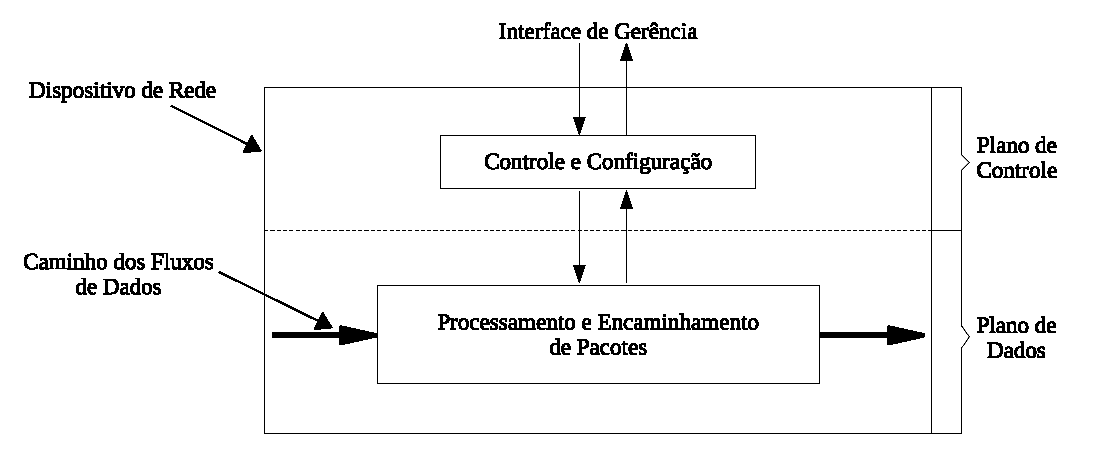
\includegraphics[width=.9\textwidth]{images/planos-introducao.eps}
  \fonte{Comer, 2013. \nocite{Comer:2013}}
  \label{fig:planos-introducao}
  
\end{figure}
\FloatBarrier

Para tentar contornar esse problema, a comunidade de pesquisa em redes de computadores tem investido em iniciativas que levem a implantação de redes com maiores recursos de programação, de forma que novas tecnologias possam ser inseridas na rede de forma gradual. Exemplos de iniciativas desse tipo são as propostas de redes ativas (\textit{active networks}) \cite{Tennenhouse:1997}, de \textit{testbeds} como o PlanetLab \cite{Chun:2003}, GENI \cite{Turner:2006} e, mais recentemente o FIBRE \cite{Salmito:2014}. Redes ativas, tiveram pouca aceitação pela necessidade de alteração dos elementos de rede para permitir que se tornassem programáveis. Iniciativas mais recentes como PlanetLab, GENI e FIBRE, apostam na adoção de recursos de virtualização para facilitar a transição para novas tecnologias. Apesar de serem consideradas de grande potencial a longo prazo, tais iniciativas ainda enfrentam desafios como garantir o desempenho exigido pelas aplicações utilizadas hoje utilizando-se tais elementos virtualizados \cite{Guedes:2006}.

Uma outra forma de abordar esse problema, consiste em estender o \textit{hardware} de encaminhamento de pacotes de forma mais restrita. Considerando-se que a operação que necessita de alto desempenho nos elementos de comutação é o encaminhamento de pacotes (plano de dados), algumas iniciativas propõem manter essa operação pouco alterada, para manter a viabilidade de desenvolvimento de hardware de alto desempenho, mas com uma possibilidade de maior controle por parte do administrador da rede. 

\gls{sdn} introduz uma perspectiva flexível para programar e manter a operacionalidade da rede  buscando desacoplar os planos de dados e de controle, desta forma, tira-se a autonomia dos equipamentos de rede que se tornam apenas encaminhadores de pacotes. Já a lógica de controle é movida para uma entidade externa, centralizada, implementada em \textit{software}. Esta, chamada de controlador, tem por funcionalidade prover a lógica de funcionamento da rede o que torna o desenvolvimento de serviços mais facilmente implementáveis, já que não há a necessidade de implementação em cada dispositivo. 

No plano de dados, o encaminhamento de pacotes, que antes era baseado em destino, passa a ser por fluxo que é definido pela combinação de campos das camadas de enlace, de rede ou de transporte, segundo o modelo TCP/IP. Dessa forma mantém-se o alto desempenho no encaminhamento de pacotes em \textit{hardware}, aliado à flexibilidade de se implementar aplicações em \textit{software}, utilizando protocolo aberto para programação da lógica do equipamento que é abstraída dos dispositivos de encaminhamento \cite{Kim:2013, Tootoonchian:2010, Rothenberg:2010}.

Pensando nisso, nasceu o OpenFlow \cite{McKeown:2008}, que por sua vez, deu origem ao conceito de \textit{Software Defined Networking}, ou redes definidas por software. A Figura \ref{fig:arch-old-sdn} apresenta um comparativo entre o modelo tradicional de rede, onde ambos os planos, de controle e de dados, são localizados em um mesmo dispositivo e o modelo \gls{sdn} que possui controle centralizado e apenas o plano de dados no dispositivo comutador.

\begin{figure}[H]
  \centering
  \caption{Modelos de rede tradicional e SDN}
  \includegraphics[width=.80\textwidth]{images/arch-old-sdn.eps}
  \fonte{Rothenberg \textit{et al.}, 2010. \nocite{Rothenberg:2010}}
  \label{fig:arch-old-sdn}
\end{figure}
\FloatBarrier

O protocolo OpenFlow é implementado em ambos os planos e dispõe de um protocolo de comunicação entre o controlador e \textit{switches}. Para garantir a confiabilidade dessa comunicação é recomendada a utilização do protocolo \gls{ssl} \cite{RFC6101} porém algumas alternativas incluem \gls{tcp}, utilizadas especialmente em redes virtuais devido à sua simplicidade, pois não necessitam de chaves criptográficas \cite{Rothenberg:2010}.

OpenFlow explora a existência de tabelas de fluxo (\textit{flow tables}) em dispositivos \textit{Ethernet} modernos. Essas tabelas são alimentadas em tempo de execução e utilizadas para implementar \textit{firewalls} \cite{Oppliger:1997}, \gls{nat} \cite{RFC3022}, \gls{qos} \cite{Aurrecoechea:1998} e coleta de estatísticas. Normalmente são proprietárias mas há um conjunto de funções que são comuns na maioria dos dispositivos. Com isso, uma forma padrão de manipulação das tabelas de fluxo pode ser implementada, independente de fornecedor. Desta maneira, OpenFlow fornece um padrão para manipulação das tabelas de fluxo, permitindo assim a partição do tráfego, o agrupamento ou isolamento da rede e o processamento ou controle do fluxo de dados, da forma desejada com base no fluxo \cite{Kontesidou:2009}.

Os principais componentes de uma arquitetura \gls{sdn} são:
\begin{itemize}
    \item Comutadores (\textit{switches}) \textit{OpenFlow};
    \item Controlador; e
    \item Protocolo de comunicação.
\end{itemize}
Estes componentes podem fazer uso do protocolo OpenFlow e/ou de outros protocolos. Por ser o primeiro e também o mais utilizado, o protocolo OpenFlow é utilizado neste trabalho como padrão de comunicação entre os dispositivos.

%=====================================================================

\subsection{Comutadores}
\label{subsec:comutador}

É o elemento responsável pelo encaminhamento dos pacotes pela rede. Pode ser específico para OpenFlow, ou ter suporte ao mesmo. No comutador (\textit{switch}) OpenFlow é mantida uma tabela de fluxo (\textit{flow table}) que armazena informações sobre como os pacotes serão processados, estatísticas, prioridades e tempo limite para novos fluxos. Além disso, cada regra é composta por um conjunto de campos do cabeçalho do pacote que podem ser visualizadas na Figura \ref{fig:flow-table}, assim como as informações de ações e estatísticas.

\begin{figure}[H]
  \centering
  \caption{Tabela de fluxo}
  \includegraphics[width=.65\textwidth]{images/flow-table.eps}
  \label{fig:flow-table}
  \fonte{Adaptado de Costa, 2014 \nocite{Costa:2004}}
\end{figure}
\FloatBarrier
%Copiado e artigo 6, reescrever
Quando um pacote chega a um equipamento com OpenFlow habilitado, os cabeçalhos do pacote são comparados (\textit{match}) às regras das entradas das tabelas de fluxos, os contadores são atualizados e as ações correspondentes são realizadas. Se não houver correspondência  (\textit{table miss}) entre o pacote e alguma entrada da tabela de fluxos, o pacote é encaminhado, por completo, ao controlador. Alternativamente, apenas o cabeçalho é encaminhado ao controlador mantendo o pacote armazenado no \textit{buffer} do \textit{hardware}. A Figura \ref{fig:fluxo-tmp} ilustra, através de um diagrama simplificado, o tratamento recebido por pacotes em um \textit{switch} OpenFlow.

Os pacotes que chegam ao controlador normalmente correspondem ao primeiro pacote de um novo fluxo ou, em função do tipo de pacote e da aplicação, o controlador pode decidir por instalar uma regra no \textit{switch} para que todos os pacotes de determinado fluxo sejam enviados para o controlador para serem tratados individualmente. Esse último caso corresponde, em geral, a pacotes de controle  (\gls{icmp} \cite{RFC0792}, \gls{dns} \cite{RFC7719}, \gls{dhcp} \cite{RFC2131}) ou de protocolos de roteamento  (\gls{ospf} \cite{RFC2328}, \gls{bgp} \cite{RFC4271}).
Todos os pacotes de uma mesma faixa de endereços \gls{ip}, ou uma conexão \gls{tcp} em determinada porta são considerados fluxos.

\begin{figure}[H]
  \centering
  \caption{Diagrama simplificado do tratamento de um pacote no \textit{switch} OpenFlow}
  \includegraphics[width=.80\textwidth]{images/flow.eps}
  \label{fig:fluxo-tmp}
  \fonte{Elaborado pelo autor a partir da especificação OpenFlow\\\cite{OpenFlowSpec:2014}}
\end{figure}
\FloatBarrier

A cada pacote recebido, é realizada a atualização dos contadores na tabela de fluxo.
Esses contadores são usados para geração de estatísticas, de maneira a monitorar o número de pacotes e bytes de cada fluxo, além do tempo de duração desde o seu início. O Quadro \ref{tab:contadores} apresenta alguns dos contadores disponíveis na tabela de fluxo. Com o auxílio deste podem ser implementados recursos de monitoramento e segurança do tráfego na rede.

\begin{table}[H]
  \centering
  %\captionof{figure}[tab:contadores]{Contadores da tabela de fluxo}
  \caption{Contadores da tabela de encaminhamento}
  \begin{tabular}{|l|c|} \hline
	\textbf{Contator} & \textbf{Tamanho em bits} \\ \hline
	\multicolumn{2}{|c|}{Por Tabela} \\ \hline
	Número de entradas Ativas & 32 \\ \hline
	Número de pacotes pesquisados & 64 \\ \hline
	Número de pacotes encontrados na tabela & 64 \\ \hline
	\multicolumn{2}{|c|}{Por fluxo} \\ \hline
	Número de pacotes recebidos & 64 \\ \hline
	Número de bytes recebidos & 64 \\ \hline
	Duração (segundos) & 32 \\ \hline
	Duração (nano segundos) & 32 \\ \hline
	\multicolumn{2}{|c|}{Por porta} \\ \hline
	Número de pacotes recebidos & 64 \\ \hline
	Número de pacotes transmitidos & 64 \\ \hline
	Número de bytes recebidos & 64 \\ \hline
	Número de bytes transmitidos & 64 \\ \hline
	Número de pacotes perdidos no recebimento & 64 \\ \hline
	Número de pacotes perdidos na transmissão & 64 \\ \hline
	Número de erros recebidos & 64 \\ \hline
  \end{tabular}
  \label{tab:contadores}
  \fonte{Elaborado pelo autor a partir da especificação OpenFlow\\  \cite{OpenFlowSpec:2014}}
\end{table}

Neste projeto o comutador a ser utilizado é o Open vSwitch \cite{website:ovs}, um \textit{switch} virtual com suporte a OpenFlow. Este comutador é projetado para permitir a automatização de grandes redes através da extensão programática, suportando ainda interfaces e protocolos de gerenciamento como, por exemplo, NetFlow \cite{rfc3954}, sFlow \cite{rfc3176} e IPFIX \cite{rfc5153}. Além disso, pode suportar a distribuição através de múltiplos servidores físicos \cite{website:ovs}.
%=====================================================================

\subsection{Controlador}
\label{subsec:controlador}

O controlador, como já citado, é o \textit{software} responsável por tomar decisões e adicionar e remover as entradas na tabela de encaminhamento, de acordo com o objetivo desejado. Exerce a função de uma camada de abstração da infraestrutura física, facilitando a criação de aplicações e serviços que gerenciem as entradas de fluxos na rede. Esse modelo assemelha-se a outros sistemas de \textit{software} que proveem abstração do \textit{hardware} e funcionalidade reutilizável. Dessa forma, o controlador atua como um \gls{so} para gerenciamento e controle das redes, e oferece uma plataforma com base na reutilização de componentes e na definição de níveis de abstração. Contudo, novas aplicações de rede podem ser desenvolvidas rapidamente \cite{Gude:2008}.

O controlador fornece uma interface para criar, modificar e controlar o fluxo de tabelas do comutador. É executado normalmente em um servidor conectado à rede e pode ser um para todos os comutadores da rede, um para cada comutador ou um para um conjunto de comutadores.  Portanto, a funcionalidade da rede de controle pode ser completamente ou localmente centralizada dependendo de como o gerenciamento dos comutadores é realizada. A exigência, no entanto, é que, se houver mais do que um controlador de processos, eles devem ter a mesma visão da topologia da rede, em qualquer momento dado. A visão de rede inclui a topologia a nível de \textit{switch}, as localizações dos usuários, \textit{hosts}, \textit{middleboxes} e outros elementos de rede e serviços. Além disso inclui todas as ligações entre os nomes e endereços.

O controlador é parte integrante de uma arquitetura de rede \gls{sdn} e para que sua comunicação com \textit{switches} OpenFlow ocorra, o controlador deve ter suporte ao mesmo. Atualmente, existem várias implementações controlador disponíveis que implementam o protocolo OpenFlow, entre os principais não comerciais estão \cite{Kreutz:2013,Xia:2015}:

\begin{itemize}
    \item \textbf{NOX} - Desenvolvido em C++, foi o primeiro controlador OpenFlow \cite{Gude:2008}. Porém não foi fortemente utilizado por causa de deficiências na sua implementação e na documentação.
    \item \textbf{POX} - Sucessor do NOX, foi desenvolvido como uma alternativa mais amigável e tem sido implementado por um grande número de engenheiros e programadores \gls{sdn}. Comparando com NOX, POX tem um ambiente de desenvolvimento mais fácil de trabalhar com uma API razoavelmente bem escrita e documentada. Também fornece uma interface Web e é escrito em Python \cite{website:pox}.
    \item \textbf{Beacon} - É um controlador SDN bem escrito e organizado. Escrito em Java, Beacon foi o primeiro controlador com o qual iniciantes pudessem trabalhar e criar um ambiente \gls{sdn}, no entanto, era limitado à topologias de rede estrela \cite{Erickson:2013}.
    \item \textbf{Floodlight} - Uma ramificação do Beacon. Enquanto que seu início tenha sido baseado no Beacon este foi desenvolvido utilizando Apache Ant, uma ferramenta popular para compilação e construção de \textit{software}, o que tornou o desenvolvimento do Floodlight mais fácil e flexível. Floodlight possui uma comunidade ativa e um grande número de recursos que podem ser adicionados ao sistema. Possui interface baseada em java e baseada em Web, além de possuir uma Interface de Programação de Aplicações (\gls{api}) \gls{rest} ou, em português, Transferência de Estado Representacional \cite{website:floodlight}.
    \item \textbf{OpenDayLight} - É um projeto colaborativo da Linux Fundation e tem sido altamente suportado por empresas como Cisco e Big Switch. Desenvolvido em Java, também inclui \gls{api} \gls{rest} e interface web. Possui suporte à \gls{sdn}, \gls{nv} , ou Virtualização de redes \cite{Chowdhury:2009} e \gls{nfv}, ou Virtualização da Funções da Rede \cite{Hawilo:2014}. Além disso, possui um grande número de módulos que podem ser utilizados para atender aos requisitos de uma organização \cite{website:odl}.
    \item \textbf{Ryu NOS} - É um \textit{framework} de \gls{sdn} baseado em componentes. O Ryu fornece componentes de software com \glspl{api} bem definidas que tornam mais fácil para os desenvolvedores criar novas aplicações de gerenciamento e controle de rede. O Ryu suporta vários protocolos para gerenciar dispositivos de rede, como OpenFlow, Netconf, OF-config, etc. Sobre o OpenFlow, o Ryu suporta totalmente as extensões 1.0, 1.2, 1.3, 1.4, 1.5 e Nicira. Todo o código está disponível gratuitamente sob a licença Apache 2.0 \cite{website:ryu}.
\end{itemize}

%=====================================================================

\subsection{Protocolo OpenFlow}
\label{subsec:protocolo-comunicacao}

O protocolo de comunicação entre os dois planos é realizado por três tipos de mensagens: controlador para o \textit{switch}, assíncrona e simétricas. 

Mensagens do tipo controlador para \textit{switch} são mensagens que o controlador envia para obter informações sobre o estado do \textit{switch}, como por exemplo verificar estatísticas de um determinado fluxo \cite{OpenFlowSpec:2014}. Essas mensagens podem ser:
%Rescrever
\begin{itemize}
    \item \textit{\textbf{Features}}: ao estabelecer uma conexão, o controlador envia esta mensagem requisitando que o \textit{switch} informe suas capacidades.
    \item \textit{\textbf{Configuration}}: o controlador envia parâmetros de configuração para os \textit{switches}. 
    \item \textit{\textbf{Modify-State}}: utilizado pelo controlador para gerenciar o estado dos \textit{switches}, deletar ou modificar regras na tabela de fluxos.
    \item \textit{\textbf{Read-State}}: utilizado pelo controlador para coletar estatísticas das tabelas de fluxos do \textit{switch}.
    \item \textit{\textbf{Packet-Out}}: utilizada pelo controlador para enviar pacotes por uma porta específica.
    \item \textit{\textbf{Barrier}}: utilizada para verificar se as dependências das mensagens foram alcançadas ou receber notificação sobre tarefas concluídas.
     \item \textit{\textbf{Role Request}}: mensagens usadas pelo controlador para configurar seu canal OpenFlow.
\end{itemize}

Mensagens assíncronas são enviadas pelo \textit{switch} sem a solicitação do controlador. \textit{Switches} enviam mensagens assíncronas para os controladores para denotar uma chegada de pacotes ou mudança de estado \cite{OpenFlowSpec:2014}. Os principais tipos de mensagens assíncronas são descritas abaixo.
\begin{itemize}
    \item \textit{\textbf{Packet-In}}: enviado pelo \textit{switch} quando há uma ação explícita na tabela de fluxos para que seja enviado para o controlador ou quando não há um \textit{match} para o pacote.
    \item \textit{\textbf{Flow-Removed}}: informa o controlador sobre a remoção de regras no \textit{switch}.
    \item \textit{\textbf{Port Status}}: informa o controlador sobre uma mudança em alguma porta.
    \item \textit{\textbf{Role Status}}: \textit{switch} informa o controlador sobre a alterações em suas regras.
    \item \textit{\textbf{Controller Status}}: \textit{switch} informa o controlador sobre a mudança em um canal OpenFlow.
    \item \textit{\textbf{Flow-monitor}}: informa o controlador sobre uma mudança na tabela de fluxo.
\end{itemize}

Finalmente, mensagens simétricas são iniciadas tanto pelo controlador como pelo \textit{switch} sem nenhuma solicitação, por exemplo o início de conexão entre controlador e \textit{switch} \cite{OpenFlowSpec:2014}. Essas mensagens são:
\begin{itemize}
    \item \textit{\textbf{Hello}}: esta mensagem é utilizada no início da conexão entre \textit{switch} e controlador.
    \item \textit{\textbf{Echo}}: utilizado para obter informações sobre a conexão entre \textit{switch} e controlador como:
latência, largura de banda e conectividade.
    \item \textit{\textbf{Error}}:  o \textit{switch} pode enviar mensagens para notificar problemas ao controlador por mensagens de erro.
    \item \textit{\textbf{Experimenter}}: na versão 1.5.0 do protocolo OpenFlow, esta mensagem é utilizada para adicionar funcionalidades experimentais.
\end{itemize}

Cada mensagem é enviada encapsulada em um pacote definido pelo protocolo OpenFlow e que é representado na Figura \ref{fig:openflow-message}.

\begin{figure}[H]
  \centering
  \caption{Formato da mensagem OpenFlow}
  \includegraphics[width=.80\textwidth]{images/openflow-message.eps}
  \label{fig:openflow-message}
  \fonte{\centering
  Elaborado pelo autor a partir de informações da especificação OpenFlow.}
\end{figure}
\FloatBarrier

O campo \textit{version} indica a versão do protocolo que está sendo utilizada. Já o  \textit{type}, indica o tipo de mensagem que está sendo enviada. O campo \textit{length} informa o tamanho da mensagem enquanto que \textit{xid} representa o ID de transação associado à mensagem. Por último, o campo \textit{payload} representa o corpo da mensagem, é neste campo onde são adicionados os diferentes tipos de mensagens apresentados anteriormente.
\section{Virtualização}
\label{sec:virtualizacao}
%Rescrever

O conceito de virtualização de redes define uma infraestrutura de redes de computadores virtuais. São definidos por \textit{software}, executando sobre máquinas físicas, de forma que toda infraestrutura virtual seja isolada da infraestrutura física, não interferindo na mesma. 

Um dos \textit{softwares} mais usados na criação de redes virtuais em nível de \textit{software} é o Xen \cite{Fernandes:2011}. Esse programa é usado na criação de máquinas virtuais em computadores pessoais e servidores, e oferece a opção de criar roteadores virtuais que podem ser utilizados na interligação de máquinas virtuais para a formação de uma rede. Em \gls{sdn} a construção de redes virtuais acontece em nível de \textit{hardware}, através da separação do tráfego da rede física em \textit{slices}, porções de fluxo do tráfego total. O FlowVisor \cite{Sherwood:2009} possibilita virtualização em \gls{sdn}.

O uso de virtualização de redes possibilita execução de experimentos distintos, sobre a mesma infraestrutura, em paralelo, sem interferência entre experimentos. Virtualização de redes também pode ser usada para isolamento de serviços. Assim, uma organização pode oferecer diversos serviços, com cada serviços executando em uma rede virtual diferente \cite{wu:2010, Mattos:2012}.

\section{Emulador Mininet}
\label{sec:mininet}

Mininet \cite{Handigol:2012} é um emulador de rede para prototipação em \gls{sdn}. A razão pela sua utilização deve-se ao fato de apenas alguns dispositivos de rede estarem disponíveis para \gls{sdn}, uma vez que ainda não é uma tecnologia difundida a nível industrial.  Além disso, a implementação de rede com elevado número de dispositivos de rede é muito difícil e dispendioso. Por isso, para contornar estes problemas, a virtualização foi realizada com a finalidade de prototipar e emular este tipo de tecnologia de rede e um dos mais importantes é o Mininet \cite{Wendong:2012}.  Mininet tem a capacidade de emular diferentes tipos de elementos de rede, tais como: \textit{host}, \textit{switches} (camada de enlace), roteadores (camada de rede) e conexões. Ele funciona em um único núcleo de Linux\cite{Negus:2015} e utiliza virtualização com a finalidade de emular uma rede completa que utiliza apenas um único sistema. No entanto, o \textit{host}, roteadores e links criados são elementos do mundo real, embora eles sejam criados por meio de software \cite{website:mininet}.

Criar uma rede no Mininet é relativamente simples. Pode-se usar linha de comando ou um componente chamado \textit{miniedit.py}, que implementa uma interface gráfica para o Mininet, este porém, possui algumas limitações em relação à linha de comando. Pela linha de comando, ao chamar o Mininet são passados os parâmetros sobre as características da rede como: topologia, número de \textit{hosts}, \textit{switches}, taxa de perda de pacotes, largura de banda, tipo de controlador, entre outros. O \textit{switch} padrão é o OpenSwitch \cite{Pettit:2010}, um \textit{switch} virtual desenvolvido especialmente para trabalhar com o protocolo Openflow. Para estudo mais aprofundado, recomenda-se a leitura da sua documentação em \cite{website:mininet}.
\section{Segurança em redes}
\label{sec:seguranca}

A segurança no nível de rede indica uma área de pesquisa muito importante, já que os usuários estão continuamente colocando seus dados em ambientes em nuvem e mais dados são transferidos através de grandes distâncias. A razão para esta evolução é a crescente popularidade dos serviços em nuvem, bem como a simplicidade e rápida capacidade dos recursos sob demanda. Os impactos variam de acordo com os tipos de ameaças, e como defesa são criados diversos sistemas de segurança que agem como barreira de proteção, como por exemplo, \textit{firewalls}. Os principais tipos de ameaças serão estudadas a seguir. Também é apresentado um estudo mais detalhado do ataque do tipo varredura, foco deste trabalho.

\subsection{Tipos de ameaças}
Dos diversos tipos de ameaças que podem ocorrer nas redes de computadores, destacam-se algumas que são notórias por causar frequentes transtornos aos usuário, tais como:

\textbf{Fraude}:
Segundo Houaiss, Villar e Francisco (2001)\nocite{Houaiss:2001}, é "qualquer ato ardiloso, enganoso, de má-fé, com intuito de lesar ou ludibriar outrem, ou de não cumprir determinado dever; logro". Esta categoria engloba as notificações de tentativas de fraudes, ou seja, de incidentes em que ocorre uma tentativa de obter vantagem, sejam por meios como correios eletrônicos não solicitados em massa (\textit{spam}) e páginas falsas.
    
\textbf{Ataque de negação de serviço (\textit{\gls{dos}}}:
Um ataque de negação de serviço busca sobrecarregar serviços na rede dificultando o seu uso por usuários legítimos. Esse tipo de ataque, por sua natureza, pode produzir variações no volume de tráfego que normalmente são visíveis no gráfico de fluxo. Segundo Sperotto \textit{et al.} (2010)\nocite{Sperotto:2010} no entanto, na detecção de intrusão por fluxo, é abordado implicitamente o problema de ataques \gls{dos} por força bruta, ou seja, um tipo de \gls{dos} que depende de esgotamento de recursos ou sobrecarga da rede. Infelizmente, é quase impossível de detectar diretamente ataques \gls{dos} semânticas.
    
\textbf{Infestações viróticas automatizadas (\textit{Worms})}:
São pequenos programas de computador criados para causar danos na máquina infectada e se auto replica pela rede, tirando cópias de si em cada computador \cite{Sperotto:2010}.
    
\textbf{Exército de máquinas controladas sem autorização (\textit{Botnets})}:
Grupo de computadores comprometidos, chamados de computadores zumbis que são controlados remotamente por um centro de controle. \textit{Botnets} são muito utilizados para lançamento de ataques  como \textit{spams}, DoS e \textit{worms} \cite{Sperotto:2010}.
    
\textbf{Varredura de portas maliciosa (\textit{port scans})}:
Técnica utilizada para encontrar fraquezas de um computador ou de uma rede. Enquanto esta técnica não é um ataque real, os hackers a usam para detectar quais portas estão abertas em um computador. Baseado nas informações sobre portas abertas, o acesso não autorizado pode ser obtido.

Os métodos citados também podem também ser utilizados em conjunto, como por exemplo a utilização de \textit{botnets} que, controlados remotamente, podem efetuar ataques DoS a um mesmo servidor e ao mesmo tempo. A esse tipo de ataque é dado o nome de Negação de Serviço Distribuída (\gls{ddos})

Do ponto de vista de segurança, existe uma quantidade crescente de incidência de ataques de negação de serviço, \gls{dos}, durante os últimos anos \cite{Seeber:2015}. Além disso, segundo a \gls{cert.br}, responsável por tratar incidentes de segurança e computadores que envolvam redes conectadas à Internet brasileira, foram reportados 722.205 incidências de segurança somente no ano de 2015, sendo mais da metade (53\%), ataques do tipo \textit{port scan}.

\subsection{Técnicas de varredura}
\label{sec:varredura}

Um dos tipos mais comuns de ataques, a varredura consiste no envio de diversos tipos de pacotes com o intuito de se conhecer mais sobre o nó alvo ou a rede em questão. Através das respostas obtidas para esses pacotes, o atacante é capaz de chegar a diversas informações que possam ajudar em futuros ataques de diversos tipos. Alguns tipos de informações que podem ser descobertas incluem (não somente): A atividade dos servidores, informações relativas a softwares utilizados no sistema, informações sobre o \textit{firewall} e topologia da rede.

Uma das principais dificuldades nas soluções desse tipo de ataque é que as varreduras são consideradas atividades legais, e ocorrem na Internet de forma rotineira, inclusive com fins não maliciosos.

Antes de explorar as técnicas de varredura, faz-se necessário o entendimento de alguns conceitos de comunicação \gls{tcp}. Para obter um serviço \gls{tcp}, uma conexão necessita ser efetivada entre os computadores origem e destino. Esta conexão é realizada através dos chamados \textit{sockets}, formados pelo par endereço \gls{ip} e número de porta, de ambos, computador de origem e computador de destino. Entre estes dois \textit{sockets} ocorre a transferência de segmentos.

Um segmento consiste em um cabeçalho \gls{tcp} seguido, opcionalmente, por informação. Um cabeçalho \gls{tcp} pode possuir seis \textit{flags} que podem ser ativadas ou desativadas ao mesmo tempo \cite{Comer:2013}, são elas:

\begin{itemize}
    \item \textbf{SYN} - \textit{bit} de sincronismo, é o \textit{bit} que informa que este é um dos dois primeiros segmentos de estabelecimento da conexão.
    \item \textbf{ACK} - \textit{bit} de reconhecimento, indica que o valor do campo de reconhecimento está carregando um reconhecimento válido.
    \item \textbf{PSH} - \textit{bit} de \textit{push}, este mecanismo, que pode ser acionado pela aplicação, informa ao \gls{tcp} origem e destino que a aplicação solicita a transmissão rápida dos dados enviados, mesmo que ela contenha um número baixo de \textit{bytes}, não preenchendo o tamanho mínimo do \textit{buffer} de transmissão.
    \item \textbf{RST} - \textit{bit} de \textit{reset}, informa o destino que a conexão foi abortada neste sentido pela origem
    \item \textbf{FIN} - \textit{bit} de terminação, indica que este pacote é um dos pacotes de finalização da conexão.
\end{itemize}

Em uma comunicação \gls{tcp}, uma conexão deve ser estabelecida entre os dois pontos (\textit{sockets}) para que a transferência de dados ocorra.
Inicialmente a máquina emissora, também chamada de cliente, transmite um segmento cuja \textit{flag} SYN é de 1 (para assinalar que se trata de um segmento de sincronização), com um número de ordem X, que se chama número de ordem inicial do cliente.

A seguir, a máquina receptora, chamada de servidor, recebe o segmento inicial que provém do cliente e envia-lhe um aviso de recepção, isto é, um segmento cuja \textit{flag} ACK é de 1 e a \textit{flag} SYN é de 1 (porque ainda se trata de uma sincronização). Este segmento contém o número de ordem do servidor, que é o número de ordem inicial do cliente. O campo mais importante deste segmento é o campo de aviso de recepção, que contém o número de ordem inicial do cliente, incrementado de 1.

Por último, o cliente transmite ao servidor um aviso de recepção, ou seja, um segmento cuja \textit{flag} ACK é de 1, cuja \textit{flag} SYN é de zero (não se trata mais de um segmento de sincronização). O seu número de ordem é incrementado e o número de aviso de recepção representa o número de ordem inicial do servidor, incrementado de 1.

Depois dessa sequência de trocas (Figura \ref{fig:troca-tcp}), também chamada de \textit{handshake}, ou, aperto de mãos em português, as duas máquinas estão conectadas e a comunicação pode ser efetivada.

\begin{figure}[H]
  \centering
  \caption{Estabelecimento de conexão TCP}
  \includegraphics[width=0.5\textwidth]{images/conexao-tcp.eps}
  \label{fig:troca-tcp}
   \fonte{Elaborado pelo autor.}
\end{figure}
\FloatBarrier

Os passos a seguir são definidos pela RFC 793 \cite{rfc793}, utilizada pela grande maioria das implementações \gls{tcp} e exploradas em técnicas de varredura.

\begin{itemize}
    \item Quando um segmento SYN chega em um aporta aberta, é continuado o procedimento de \textit{handshake} como discutido anteriormente; 
    \item Quando um segmento SYN (ou FIN) chega em uma porta fechada, o segmento é descartado e um segmento RST é retornado para o cliente;
    \item Quanto um segmento FIN chega em uma porta que esteja aberta, o segmento é descartado.
    \item Quando um segmento RST chega em uma porta que esteja ouvindo (aberta), o segmento é descartado;
    \item Quando um segmento RST chega em uma porta que não esteja ouvindo (fechada), o segmento é descartado;
    \item Quando um segmento ACK chega à uma porta aberta, o mesmo é descartado e retornado um segmento RST.
\end{itemize}


Devido à sua natureza, \textit{scans} podem facilmente criar um vasto número diferente de fluxos. Segundo Speroto \textit{et al.} (2010)\nocite{Sperotto:2010}, há três categorias de varredura, são elas:
\begin{itemize}
    \item \textbf{\textit{scan} horizontal} - quando um \textit{host} de origem varre uma porta especifica em diferentes \textit{hosts} alvo;
    \item \textbf{\textit{scan} vertical} - quando um \textit{host} de origem verifica várias portas distintas de um mesmo \textit{host} alvo; e
    \item \textbf{\textit{scan} misto} - quando há a combinação das varreduras vertical e horizontal.
\end{itemize}

Existem várias técnicas de varredura de porta disponíveis e podem facilmente ser automatizadas por ferramentas como Nmap \cite{Lyon:2009}. Alguns métodos utilizados para varredura são estudados a seguir \cite{deVivo:1999, Christopher:2001}.
\begin{itemize}
\item \textbf{\textit{TCP Connect}} - É a forma mais comum de \textit{scanning}. Basicamente uma conexão TCP regular (\textit{handshake} completo) para cada porta definida na varredura. Para cada porta, a conexão pode resultar em sucesso, indicando uma porta aberta ou em falha caso contrário. Essa técnica é facilmente implementada pois não necessita de privilégios especiais e, do mesmo modo, é facilmente detectável. Através de \textit{logs} do sistema alvo é possível verificar mensagens de requisição de conexão e de erro para as conexões negadas. Neste método, o \textit{scanner} envia uma mensagem SYN para o sistema alvo. Se uma porta estiver (aberta) ouvindo com um serviço, a conexão se sucederá. Um SYN é retornado estabelecendo o número de sequência inicial. Um ACK considera o campo numérico de confirmação válido. Se a porta estiver (fechada) sem serviço ouvindo, uma mensagem RST é retornada, para reiniciar o pedido de conexão. Alguns exemplos de \textit{scanners} podem ser Nmap, Amap e Blaster. %Exemplo de \textit{scanner}: nmap.

\item \textbf{TCP SYN} - Também conhecida por \textit{Half Open} por não explorar um \textit{handshake} completo. Nesta técnica o \textit{scanner} envia uma mensagem SYN, como se estivesse pedindo uma conexão. Se responder como um RST, indica que a porta está fechada, e uma nova porta é testada. Se a resposta da máquina alvo for um SYN/ACK, indica que a porta se encontra ouvindo. O \textit{scanner} envia então um RST cancelando o \textit{handshake}. A vantagem desse tipo de \textit{scanning} é o fato de, mesmo ainda podendo ser detectado, tentativas de conexões SYN são menos frequentemente registradas se comparadas com conexões \gls{tcp} completas. %Exemplos de \textit{scanners}: amap, hping2, netstat, nmap.

\item \textbf{Exploração FIN} - Neste método, quando um segmento FIN é enviado para uma porta fechada, o computador alvo responde com um TCP RST. Quando a porta estiver aberta, o segmento é ignorado e o computador alvo não responde. O \textit{scanner} não recebe nunhuma resposta, pois não podem pertencer a uma conexão estabelecida. %Exemplos de \textit{scanners}: hping2, nmap.

\item \textbf{Xmas Tree} - é uma variação do método TCP FIN, neste, são utilizadas mensagens com prioridade TCP FIN/URG/PSH. Quando estiver ouvindo, o \textit{host} alvo não responde, caso contrário, responde com um TCP RST. %Exemplos de \textit{scanners}: hping2, netstat, nmap.

\item \textbf{TCP Null (sem flags ativos)} - também é uma variação do método TCP FIN, neste, tem-se resposta para portas fechadas, mas não para portas abertas.% Exemplos de \textit{scanners}: hping2, netstat, nmap.

\item \textbf{Varredura ACK} - Técnica utilizada para identificar \textit{firewalls}. Um segmento ACK que não pertença a nenhum conexão é gerado pelo \textit{scanner}. Se um RST é devolvido pela máquina alvo, tanto em uma porta aberta como em uma fechada, as portas são classificadas como não tendo \textit{firewall}.

\item \textbf{Varredura ARP} - Não se trata exatamente de varredura de portas mas essa técnica é utilizada para descobrir dispositivos ativos na rede local, para depois realizar a varredura de portas somente nos computadores ativos. O \textit{scanner} envia uma série de pacotes de protocolo \gls{arp} \cite{RFC0826} e incrementa o valor do \gls{ip} alvo a cada \textit{broadcast}.
\end{itemize}


\subsection{Ferramentas de Varredura}

Para que as varreduras sejam efetuadas, tem-se a possibilidade de utilizar ferramentas que possibilite a varredura utilizando as diferentes formas citadas na seção anterior. Uma das ferramentas mais utilizadas, e que foi utilizada neste trabalho é o Nmap \cite{Lyon:2009}.

O Nmap é um \textit{software} que oferece uma gama muito grande de recursos e funcionalidades, como detecção do Sistema Operacional remoto, o serviço e a versão que está em uso no host, o exame de ociosidade por identificação (ID) de Internet Protocol (IP), o rápido exame de multiportas por ping entre tantas outras. Possui versões para plataformas Unix, Windows, e MacOS sendo utilizado tanto por interface console como também em interface gráfica, o software Nmap é um utilitário livre e de código aberto, usado para exploração de redes, segurança e auditoria, capaz de examinar grandes redes ou simplesmente um único host.
A função principal do Nmap é realizar uma varredura em portas \gls{tcp} e o retorno dessa varredura é classificado em um dos seguintes estados: aberta, fechada, filtrada, nao filtrada e a combinação de aberta/filtrada ou fechada/filtrada \cite{Lyon:2009}. Vários outros softwares que são utilizados para gerencia e controle de redes de computadores fazem uso do Nmap pois pode ser usado diretamente, sempre que se desejar uma verificação de portas em um \textit{host} que esteja em uma rede local ou na Internet.
O uso mais simples do Nmap é escanear diretamente uma máquina da rede, onde uma quantidade enorme de portas \gls{tcp} será examinada na máquina alvo, e cada porta será classificada de acordo com seu estado.
Na linha de comando do Nmap, tudo que não for uma opção ou argumento de opção será tratado como uma especificação de hospedeiro alvo. O caso mais simples é a especificação de um endereço IP ou nome de hospedeiro alvo para exame \cite{Lyon:2009}.


\subsection{Sistemas de detecção e prevenção de intrusão}

O isolamento da rede em redes virtuais permite uma maior segurança devido ao seu isolamento, porém problemas tradicionais relacionados à segurança continuam existindo em ambientes virtualizados pois 60\% a 70\% dos ataques à segurança da rede são de origem interna segundo Lynch (2006)\nocite{Lynch:2006}. Uma das formas de se proteger desses ataques é monitorar o tráfego em busca de atividades maliciosas ou violação de políticas. Para realizar o monitoramento de pacotes na rede, a solução mais apropriada é o sistema de detecção de intrusão, que realiza o monitoramento passivo dos pacotes na rede. Porém, esse tipo de análise não permite que sejam tomadas ações para prevenir tais ataques, e então faz se necessário um sistema de prevenção de intrusão para bloquear esses pacotes.

Segundo Kruegel (2004)\nocite{Kruegel:2004}, "Detecção de intrusão é o processo de identificar e responder à atividades maliciosas na computação e redes de dados". Uma tentativa de intrusão, também chamada de ataque, refere-se a uma série de ações em que um intruso tenta obter o ganho do sistema e o objetivo de um \gls{ids} é discriminar tentativas de intrusão e preparação de intrusão do uso normal do sistema.

Em redes tradicionais, para detectar e prevenir intrusos maliciosos na rede de dados, administradores normalmente necessitam implantar diversos detectores de intrusão em diferentes locais da rede, e então analisar dados do tráfego coletados localmente ou em um nodo centralizado. Infelizmente, arquiteturas \gls{ids}/\gls{ips} utilizadas atualmente possuem muitas barreiras para gerir nós distribuídos. Em primeiro lugar, os nós de detecção de intrusão devem suportar diferentes configurações. Como as configurações dependem da topologia da rede, configurações manuais e mudanças frequentes são inevitáveis para tornar a política em nós distribuídos eficaz e coerente. Em segundo lugar, algoritmos de detecção de intrusão eficazes normalmente são desenhados para um determinado tipo de ataque. Para desenvolver sistemas de detecção eficazes, mais e mais protocolos de proteção são criados, o que resulta na redução do desempenho da rede. Além disso, dispositivos de rede normalmente possuem protocolos proprietários, o que torna mais difícil desenvolver interfaces de gerenciamento automáticas \cite{Wang:2015}.

Vários trabalhos para \gls{ids} tem sido desenvolvidos desde o início de sua pesquisa nos anos 1980. Essas propostas podem ser classificadas de acordo com várias características, como tipo de dados analisado (\textit{logs} ou dados do pacote), tipo de análise (em tempo real ou \textit{offline}) ou pelo tipo de processamento (centralizado ou distribuído). No entanto, os modelos de classificação mais conhecidos são os baseados em assinatura e os baseados em anomalia \cite{Axelsson:2000}.

Sistemas de detecção de intrusão baseados em assinatura realizam a detecção através da comparação de dados do pacote com uma base de dados conhecida. O \gls{ids} Snort \cite{Roesch:1999} é um dos exemplos mais utilizados dessa técnica, verificando padrões de pacote através da análise de dados da carga útil (\textit{payload}) do pacote. O Snortik \cite{Fagundes16} também é um bom exemplo, neste, é proposto uma integração entre o \gls{ids} Snort e o sistema de \textit{firewall} do sistema MikroTik RouteOS \cite{mikrotik16} com a finalidade de automatizar o processo de reação à ataques. \glspl{ids} baseados em assinatura possuem alta precisão, raramente apresentando alarmes para fluxos normais, porém, não reconhecem fluxos novos, não presentes na sua base de dados. Além disso, a inspeção de pacotes é difícil e até mesmo impossível de ser realizada  em redes com taxas com múltiplos Gigabits por segundo \cite{Lai:2004, Gao:2006}.

Sistemas de detecção de intrusão baseados em anomalia por sua vez, comparam dados recebidos com um "modelo de normalidade" que descreve o comportamento normal da rede. Alterações significativas desse modelo são consideradas como anomalias. Exemplos de criação de comportamentos podem ser redes neurais, técnicas de análise de estatísticas e teoria das probabilidades. A principal vantagem desse tipo de detecção é o fato de também detectar fluxos não conhecidos anteriormente \cite{Owezarski:2010}. No entanto, podem existir casos em que fluxos podem ser diferentes da normalidade esperada mas não necessariamente serem maliciosos resultando em alarmes falsos positivos.

Um \gls{ids} deve ser capaz de lidar com o número crescente do tráfego e ataques na rede. No entanto, alternativas baseadas nas análise de carga útil possuem eficácia em redes entre 100Mbps e 200Mbps \cite{Lai:2004, Gao:2006} podendo chegar a 1Gbps quando hardware dedicado é empregado \cite{Vasiliadis:2008}. Sistemas como Bro \cite{Paxson:1999} e Snort \cite{Roesch:1999} apresentam alto consumo de recursos  quando confrontado com a enorme quantidade de dados de alta taxa de transferência encontrados atualmente \cite{Dreger:2004}. Além disso, protocolos criptografados podem representar um desafio a mais para sistemas de carga útil. Para redes de alta taxas de transmissão, alternativas à inspeção de pacotes são muito importantes. Uma dessas alternativas e que tem atraído pesquisadores é a detecção de intrusão de anomalias baseada em fluxo.

Com esta abordagem, são analisados os padrões de comunicação dentro da rede, ao invés do conteúdo dos pacotes individuais. Hoje em dia os sistemas de medição especiais são capazes de fornecer, para cada par de endereços IP e números de porta, informações agregadas, como a quantidade de bytes transferidos, o número de pacotes enviados e o tempo que determinado fluxo de dados esteve ativo. Essas informações podem então ser exportadas para outros sistemas analisarem, para então, serem usados para detectar intrusões \cite{Sperotto:2010}.

Considerando essa inflexibilidade sobre os equipamentos atuais, os interesses sobre abstrair funções de rede de \textit{switches} dedicados para aplicações \gls{sdn} vem aumentando. Sendo assim, as políticas de segurança podem ser instaladas pelo controlador como regras nas tabelas de fluxo \cite{Kim:2013}, em vez de configurações manuais e independentes. Com isso, o \textit{switch} provê apenas a função de filtro de acordo com a regra na tabela de fluxo, não influenciando significativamente no desempenho da rede. Além disso, \gls{sdn} tem recursos naturais de estatísticas que são úteis para a análise de detecção de intrusão, de modo que o controlador obtém mais visibilidade sobre o tráfego da rede. Portanto, \gls{sdn} parece fornecer uma arquitetura mais adequada para \gls{ips}.




%------------------------------------------
%Referencias
\bibliography{referencias}

% Anexos

\end{document}
